\chapter{Algunas aplicaciones de la integración}

\setcounter{section}{1}
\section{El área de una región comprendida entre dos gráficas expresada como una integral}

%--------------------2.1
\begin{teo} Supongamos que $f$ y $g$ son integrables y que satisfacen $f\leq q$ en $[a,b]$. La región $S$ entre sus gráficas es medible y su área $a(S)$ viene dada por la integral $$a(S) = \int_a^b [g(x)-f(x)] \; dx$$
    Demostración.- \; 
	Demostración.- \; Supongamos primero que $f$ y $g$ son no negativas,. Sean $F$ y $G$ los siguientes conjuntos:
	$$F = {(x,y)|a\leq x \leq b, 0\leq y \leq f(x)}, \quad G = {(x,y) | a\leq x \leq b, 0\leq y \leq g(x)}.$$
	Esto es, $G$ es el conjunto de ordenadas de $g$, y $F$ el de $f$, menos la gráfica de $f$. La región $S$ es la diferencia $G-F$. Según los teoremas 1.10 y 1.11, $F$ y $G$ son ambos medibles. Puesto que $F \subseteq G$ la diferencia $S = G-F$ es también medible, y se tiene 
	$$a(S) = a(G) - a(F) = \int_a^b g(x) \; dx = \int_a^b [g(x)-f(x)] \; dx$$
	Consideremos ahora el caso general cuando $f\leq q$ en $[a,b]$, pero no son necesariamente no negativas. Este caso lo podemos reducir al anterior trasladando la región hacia arriba hasta que quede situada encima del eje $x$. Esto es, elegimos un número positivo $c$ suficientemente grande que asegure que $0 \leq f(x) + c \leq g(x) + c$ para todo $x$ en $[a,b]$. Por lo ya demostrado la nueva región $T$ entre las gráficas de $f+c$ y $g+c$ es medible, y su parea viene dad por la integral
	$$a(T) = \int_a^b [(g(x)+c) - (f(x)+c)] = \int_[g(x)-f(x)] \; dx$$
	Pero siendo $T$ congruente a $S$, ésta es también medible y tenemos $$a(S) = a(T) = \int_a^b [g(x) - f(x)]\; dx$$
	Esto completa la demostración.\\\\
\end{teo}

%----------nota 2.1
    \begin{nota} En los intervalos $[a,b]$ puede descomponerse en un número de subintervalos en cada uno de los cuales $f\leq g$ o $g\leq f$ la fórmula (2.1) del teorema 2.1 adopta la forma 
    $$a(S) = \int_a^b |g(x) -f(x)| \; dx$$
    \end{nota}

    %--------------------lema 2.1
    \begin{lema}[Área de un disco circular] Demostrar que $A(r) = r^2 A(1)$. Esto es, el área de un disco de radio $r$ es igual al producto del área de un disco unidad (disco de radio $1$) por $r^2$.\\\\
	Demostración.-\; Ya que $g(x) - f(x) = 2g(x),$ el teorema 2.1 nos da 
	    $$A(r) = \int_{-r}^r g(x) \; dx = 2 \int_{-r}^r \sqrt{r^2 - x^2} \; dx$$
	    En particular, cuando $r = 1$, se tiene la fórmula $$A(1) = 2\int_{-1}^1 \sqrt{1 - x^2} \; dx$$
	    Cambiando la escala en el eje $x$, y utilizando el teorema 1.19 con $k=1/r$, se obtiene
	    $$A(r) = 2\int_{-r}^r g(x) \; dx = 2r \int_{-1}^1 g(rx) \; dx = 2r\int_{-1}^1 \sqrt{r^2 - (rx)^2} \; dx = 2r^2 \int_{-1}^1 \sqrt{1-x^2} \; dx = r^2 A(1)$$
	    Esto demuestra que $A(r) = r^2 A(1)$, como se afirmó.\\\\
    \end{lema}

%---------------------definición 2.1
    \begin{def.} Se define el número $\pi$ como el área de un disco unidad.
	$$\pi = 2 \int_{-1}^1 \sqrt{1-x^2}\; dx$$
    \end{def.}
\begin{center}
    La formula que se acaba de demostrar establece que $A(r) = \pi r^2$\\
\end{center}

Generalizando el anterior lema se tiene 
    $$a(kS) = \int_{ka}^{kb} g(x)\; dx = k \int_{ka}^{kb} f(x/k) \; dx = k^2 \int_a^b f(x) \; dx$$

%--------------------teorema 2.1
\begin{teo} Para $a>0$, $b>0$ y $n$ entero positivo, se tiene $$\int_a^b x^{\frac{1}{n}} \; dx = \dfrac{b^{1-1/n} - a^{1-\frac{1}{n}}}{1+\frac{1}{n}}$$\\
    Demostración.-\; Sea $\int_0^a x^{\frac{1}{n}}$. El rectángulo de base $a$ y altura $a^{\frac{1}{n}}$ consta de dos componentes: el conjuntos de ordenadas de $f(x) = x^{\frac{1}{n}}$ a $a$ y el conjuntos de ordenadas $g(y) = y^n$ a $a^{\frac{1}{n}}$. Por lo tanto,
    $$a\cdot a^{\frac{1}{n}} = a^{1+\frac{1}{n}} = \int_0^a x^{\frac{1}{n}} \; dx + \int_0^{a^{\frac{1}{n}}} y^n \; dy \; \Longrightarrow \; \int_0^a x^{\frac{1}{n}} \; dx = a^{1+\frac{1}{n}} - \dfrac{y^{n+1}}{n+1}\bigg|_0^{a^{\frac{1}{n}}} = a^{1+\frac{1}{n}} -  \dfrac{a^{1+\frac{1}{n}}}{n+1} = \dfrac{a^{1+\frac{1}{n}}}{1 + 1/n}$$
    Análogamente se tiene $$\int_0^b x^{\frac{1}{n}}\; dx = \dfrac{b^{1 + \frac{1}{n}}}{1 + 1/n}$$
    Luego notemos que $$\int_a^b x^{\frac{1}{n}} \; dx = \int_0^b x^{\frac{1}{n}}\; dx - \int_0^a x^{\frac{1}{n}} \;dx$$
    por lo tanto $$\int_a^b x^{\frac{1}{n}}\; dx = \dfrac{b^{1+\frac{1}{n}} - b^{1 + \frac{1}{n}}}{1 + 1/n}$$\\\\
\end{teo}



\setcounter{section}{3}
\section{Ejercicios}

En los ejercicios del 1 al 14, calcular el área de la región $S$ entre las gráficas de $f$ y $g$ para el intervalo $[a,b]$ que en cada caso se especifica. Hacer un dibujo de las dos gráficas y sombrear $S$.\\

\begin{enumerate}[\bfseries 1.]

%--------------------1.
\item $f(x) = 4 - x^2, \quad g(x)=0, \quad a = -2, \quad b = 2$\\\\
    Respuesta.-\; $$\int_{-2}^2 [4-x^2 - 0] \; dx = 4x \bigg|_{-2}^2 -\dfrac{x^3}{3}\bigg|_{-2}^2 = 4(2-(-2)) - \left(\dfrac{2^3 - (-2)^3}{3}\right)  = \dfrac{32}{3}$$\\ 

%--------------------2.
\item $f(x) = 4 - x^2, \quad g(x) = 8 - 2x^2,\quad a = -2, \quad b = 2.$\\\\
    Respuesta.-\; $$\int_{-2}^2 [8 - 2x^2 - (4 - x^2)] \; dx = \int_{-2}^2 4-x^2 \; dx = \dfrac{32}{3} \; (por \, ejercicio \; 1)$$\\

%--------------------3.
\item $f(x)=x^3+x^2,\quad g(x)=x^3 + 1, \quad a=-1, \quad b=1$.\\\\
    Respuesta.-\; $$\int_{-1}^1 x^3 + 1 - (x^3 + x^2) \;dx = \int_{-1}^1 1-x^2\; dx = x\bigg|_{-1}^1 - \dfrac{x^3}{3}\bigg|_{-1}^1   = 2 - \dfrac{1-(-1)}{3} = \dfrac{4}{3}$$\\

%--------------------4.
\item $f(x)=x-x^2,\quad g(x)=-x,\quad a=0,\quad b=2$\\\\
    Respuesta.-\; $$\int_0^2 x-x^2 - (-x) \; dx = \int_0^2 2x - x^2 = 2\dfrac{x^2}{2}\bigg|_0^2 - \dfrac{x^3}{3}\bigg|_0^2 = 2\dfrac{2^2}{2} - \dfrac{2^3}{3} = \dfrac{4}{2}$$\\

%--------------------5.
\item $f(x) = x^{1/3}, \quad g(x) = x^{1/2}, \quad a=0, \quad b=1$\\\\ 
    Respuesta.-\; $$\int_0^1 x^{1/3} - x^{1/2} \; dx = \dfrac{x^{1+1/3}}{1+1/3}\bigg|_0^1 - \dfrac{x^{1+1/2}}{1+1/2}\bigg|_0^1 = \dfrac{3}{4} - \dfrac{2}{3} = \dfrac{1}{12}$$\\

%--------------------6.
\item $f(x) = x^{1/3}, \quad g(x) = x^{1/2},\quad a=1,\quad b=2.$\\\\
    Respuesta.-\; $$\int_1^2 x^{1/2}-x^{1/3}\; dx = \dfrac{x^{1/2 + 1}}{1 + 1/2}\bigg|_1^2 - \dfrac{x^{1/3}+1}{1+1/3}\bigg|_1^2 = \dfrac{2^{1/2+1}-1}{1+1/2}-\dfrac{2^{1/3+1}}{1+1/3} = \dfrac{4\sqrt{2}}{3}-\dfrac{3\sqrt[3]{2}}{2}+\dfrac{1}{12}$$\\

%--------------------7.
\item $f(x)=x^{1/3},\quad g(x) = x^{1/2}, \quad a = 0,\quad b=2$\\\\
    Respuesta.-\; Sea $$\int_0^1 |x^{1/3}-x^{1/2}|\; dx + \int_1^2 |x^{1/3}-x^{1/2}|\; dx$$
    por los problemas 5 y 6 se tiene $$\dfrac{1}{12} + \dfrac{4\sqrt{2}}{3}-\dfrac{3\sqrt[3]{2}}{2}+\dfrac{1}{12} = \dfrac{4\sqrt{2}}{3}-\dfrac{3\sqrt[3]{2}}{2}+\dfrac{1}{6}$$\\

%--------------------8.
\item $f(x) = x^{1/2}, \quad g(x) = x^2, \quad a=0, \quad b=2$\\\\
    Respuesta.-\;
    \begin{center}
	\begin{tabular}{rcl}
	    $\displaystyle\int_0^1 x^{1/2} - x^2 \; dx + \int_1^2 x^2 - x^{1/2}\; dx$ & $=$ & $\left(\dfrac{x^{1+1/2}}{1+1/2}\bigg|_0^1 - \dfrac{x^3}{3}\bigg|_0^1\right) + \left( \dfrac{x^3}{3}\bigg|_1^2 - \dfrac{x^{1+1/2}}{1+1/2}\bigg|_1^2 \right)$\\\\
	    & $=$ & $\left(\dfrac{1}{1+1/2} - \dfrac{1}{3}\right) + \left(\dfrac{2^3-1}{3} - \dfrac{2^{1+1/2} - 1}{1+1/2}\right)$\\\\
	    & $=$ & $\dfrac{2}{3} - \dfrac{1}{3} + \dfrac{7}{3} - \dfrac{4\sqrt{2}-2}{3}$\\\\
	    &$=$&$\dfrac{10}{3}-\dfrac{4\sqrt{2}}{3}$\\\\
	\end{tabular}
    \end{center}

%--------------------9.
\item $f(x) = x^2, \quad g(x) = x+1, \quad a=-1, \quad b = (1+\sqrt{5})/2$\\\\
    Respuesta.$$\int_{-1}^{(1-\sqrt{5})/2} x^2 - (x+1)\; dx +  \int_{(1-\sqrt{5})/2}^{(1+\sqrt{5})/2} (x+1) - x^2\; dx-\; = $$
    \begin{center}
	\begin{tabular}{rcl}
	     & $=$ & $\displaystyle\int_{-1}^{(1-\sqrt{5})/2} x^2 - x - 1\; dx +  \int_{(1-\sqrt{5})/2}^{(1+\sqrt{5})/2} x + 1 - x^2 \; dx$ \\\\
	    & $=$ & $\left(\dfrac{x^3}{3} - \dfrac{x^2}{2} - x\right)\bigg|_{-1}^{(1-\sqrt{5})/2} + \left(\dfrac{x^2}{2} + x - \dfrac{x^3}{3}\right)\bigg|_{(1-\sqrt{5})/2}^{(1+\sqrt{5})/2}$ \\\\
	    & $=$ & $-\dfrac{3}{4} + \dfrac{5 \sqrt{5}}{12}+\dfrac{5\sqrt{5}}{6}$ \\\\
	    & $=$ & $\dfrac{5\sqrt{5}-3}{4}$\\\\
	\end{tabular}
    \end{center}

%--------------------10.
\item $f(x)=x(x^2-1),\quad g(x)=x,\quad a=-1, \quad b=\sqrt{2}$\\\\
    Respuesta.-\; $$\int_{-1}^{0} x(x^2-1) - x \; dx + \int_{0}^{\sqrt{2}} x - [x(x^2-1)] \; dx = \int_{-1}^{0} x^3-2x \; dx + \int_{0}^{\sqrt{2}} - x^3 + 2x \; dx = $$
	$$=\left(\dfrac{x^4}{4} - x^2 \right)\bigg|_{-1}^0 + \left( -\dfrac{x^4}{4} + x^2 \right)\bigg|_{0}^{\sqrt{2}} = -\dfrac{1}{4} + 1 + (-1+2) = \dfrac{7}{4}$$\\

%--------------------11.
    \item $f(x)=|x|,\quad g(x) = x^2-1, \quad a=-1,\quad b=1$\\\\
	Respuesta.-\; Definimos $f$ de la siguiente manera: $$f(x) = |x| = \left\{\begin{array}{rcl}
	    -x&si&x\in [-1,0)\\
	    x&si&x\in [0,1]\\
	    \end{array}\right.$$
	    Luego,
	    \begin{center}
	    \begin{tabular}{rcl}
		$\displaystyle\int_{-1}^1 f(x)-g(x) \; dx$ & $=$ & $\displaystyle\int_{-1}^0 -x-x^2+1 \; dx + \int_0^1 x-x^2+1 \; dx$\\\\
		& $=$ & $ \left(-\dfrac{x^2}{2}-\dfrac{x^3}{3} + x \right) \bigg|_{-1}^0 + \left(\dfrac{x^2}{2} - \dfrac{x^3}{3} + x\right)\bigg|_0^1 $\\\\
		& $=$ & $\left(\dfrac{1}{2} - \dfrac{1}{3}+1\right)+\left(\dfrac{1}{2}-\dfrac{1}{3} + 1\right)$\\\\
		& $=$ & $\dfrac{7}{3}$ \\\\
	    \end{tabular}
	    \end{center}

%--------------------12.
\item $f(x) = |x+1|,\quad g(x)=x^2-2x, \quad a=0, \quad b=2$\\\\
    Respuesta.- \; Definamos $f$ de la siguiente manera:
	$$f(x)= |x-1| = \left\{
	    \begin{array}{rcl}
		-(x+1)&si&x\in[0,1)\\
		x+1&si&x\in [1,2]\\
	    \end{array}
	    \right.$$
	    Entonces, 
	    \begin{center} 
		\begin{tabular}{rcl}
		    $\displaystyle\int_0^2 f(x)-g(x) \; dx$&$=$&$\displaystyle\int_0^1 -(x-1)-x^2+2x\; dx + \int_1^2 x-1-x^2+2x \; dx$\\\\
		    & $=$ &$\displaystyle\int_0^1 -x^2+x+1\; dx + \int_1^2 -x^2+3x - 1 \; dx$\\\\
		    & $=$ & $\left(-\dfrac{x^3}{3} + \dfrac{x^2}{2} + x\right)\bigg|_0^1 + \left(-\dfrac{x^3}{3} + \dfrac{3x^2}{2} -x\right)\bigg|_1^2$\\\\
		    & $=$ & $\left(-\dfrac{1}{3} + \dfrac{1}{2} + 1\right)+\left(-\dfrac{8}{3} + 6-2+\dfrac{1}{3} -\dfrac{3}{2} + 1\right)$\\\\
		    & $=$ & $\dfrac{7}{3}$\\\\
		\end{tabular}
	    \end{center}

%--------------------13.
\item $f(x) = 2|x|, \quad g(x) = 1-3x^3, \quad a=-\sqrt{3}/3, \quad b=\dfrac{1}{3}$\\\\ 
    Respuesta.-\; Definimos $f$ de la siguiente manera: $$f(x) = |x| = \left\{\begin{array}{rcl}
	-x&si&x\in [-\sqrt{3}/3,0)\\
	    x&si&x\in [0,1/3]\\
	    \end{array}\right.$$
	    de donde se tiene,
	    \begin{center}
		\begin{tabular}{rcl}
		    $\displaystyle\int_{-\frac{\sqrt{3}}{3}}^{\frac{1}{3}} g(x)-f(x)\; dx$ & $=$ & $\displaystyle\int_{-\frac{-\sqrt{3}}{3}}^{\frac{1}{3}}g(x) \; dx - \int_{-\frac{\sqrt{3}}{3}}^{\frac{1}{3}} f(x) \; dx$\\\\\
		    & $=$ & $\displaystyle\int_{-\frac{\sqrt{3}}{3}}^{\frac{1}{3}} 1-3x^3 \; dx - \int_{-\frac{\sqrt{3}}{3}}^{0} -2x \; dx - \int_{0}^{\frac{1}{3}} 2x \; dx$\\\\
		    & $=$ & $\left(x-\dfrac{3}{4} x^4\right)\bigg|_{-\frac{\sqrt{3}}{3}}^{\frac{1}{3}} + x^2 \bigg|_{-\frac{\sqrt{3}}{3}}^{0} - x^2 \bigg|_0^{\frac{1}{3}}$\\\\
		    & $=$ & $\left(\dfrac{1}{3} - \dfrac{1}{108} + \dfrac{\sqrt{3}}{3} + \dfrac{1}{12}\right)+\left(-\dfrac{1}{3}\right)-\dfrac{1}{9}$\\\\
		    & $=$ & $\dfrac{9\sqrt{3}-1}{27}$\\\\
		\end{tabular}
	    \end{center}


%--------------------14.
\item $f(x) = |x|+|x-1|, \quad g(x)=0, \quad a=-1,\quad b=2$\\\\
    Respuesta.-\; En este problema $f(x)\geq g(x)$ en el intervalo $[-1,2]$, por lo tanto 
    $$\int_{-1}^2 f(x)-g(x)\; dx = \int_{-1}^2 |x| + |x+1|\; dx = \int_{-1}^2 |x|\; dx + \int_{-1}^2 |x-1| \; dx$$
    Definimos cada función por separado,
    $$|x| = \left\{ \begin{array}{rcl} -x & si & x\in [-1,0)\\ x & si & x\in [0,2] \end{array}\right.$$
    $$|x-1| = \left\{ \begin{array}{rcl} -(x-1) & si & x\in [-1,1)\\ x-1 & si & x\in [1,2] \end{array}\right.$$
    por lo tanto
    \begin{center}
	\begin{tabular}{rcl}
	    $\displaystyle\int_{-1}^2 |x|\; dx + \int_{-1}^2 |x-1|\; dx$&$=$&$\displaystyle\int_{-1}^0 -x \; dx + \int_0^2 x\; dx + \int_{-1}^1 -(x-1)\; dx + \int_1^2 x-1\; dx$\\\\
	    &$=$&$\left(-\dfrac{x^2}{2}\right)\bigg|_{-1}^0 + \left(\dfrac{x^2}{2}\right)\bigg|_{0}^2 + \left(-\dfrac{x^2}{2}\right)\bigg|_{-1}^1 + \left(x\right)\bigg|_{-1}^1 + \left(\dfrac{x^2}{2}\right)\bigg|_{1}^2 + \left(-x\right)\bigg|_{1}^2$\\\\\
	    &$=$&$\dfrac{1}{2}+2-\dfrac{1}{2}+\dfrac{1}{2}+1+1+2-\dfrac{1}{2}-2+1$\\\\\
	    &$=$&$5$\\\\\
	\end{tabular}
    \end{center}

%--------------------15.
\item Las gráficas de $f(x) = x^2$ y $g(x)=cx^3$, siendo $c>0$, se cortan en los puntos $(0,0)$ y $(1/c,1/c^2)$. Determinar $c$ de modo que la región limitada entre esas gráficas y sobre el intervalo $[0,1/c]$ tengan área $\frac{2}{3}$.\\\\
    Respuesta.-\; Tenemos que $f\geq g$ en el intervalo $[0,1/c]$ de donde, 
    $$\int_0^{1/c} x^2 -cx^3 \; dx = \int_0^{1/c} x^2\; dx - c\int_0^{1/c} x^3 \; dx = \dfrac{1}{12c^3}$$
    luego $\dfrac{1}{12c^3}=\dfrac{2}{3}$ por lo tanto $c=\dfrac{1}{2}$.\\\\

%--------------------16.
\item Sea $f(x)=x-x^2$, $g(x) = ax$. Determinar $a$ para que la región situada por encima de la gráfica de $g$ y por debajo de $f$ tenga área $frac{9}{2}$.\\\\
    Respuesta.-\; Tomaremos los casos cuando $a=0, a>0$ y $a<0$. \\
    Veamos primero que si $g(x)\leq f(x)$ entonces $$f(x)-g(x)\geq 0 \Longrightarrow x-x^2-ax\geq 0 \Longrightarrow (1-a)x \geq x^2$$
    de donde si $x=0$ se tiene una igualdad. Luego si $x\neq 0$ entonces $x\leq (1-a)$. Ahora sea $a<0$ por suposición se tendrá $1-a>0$, que nos muestra que el intervalo estará dado por $[0,1-a]$. Análogamente se tiene el intervalo $[1-a,0]$ para $a>0$.\\
    \begin{enumerate}[\bfseries C 1.]
	\item Si $a=0$, esto no es posible ya que si $a = 0$ entonces $g(x) = ax = 0$ y entonces el área arriba del gráfico de $g$ y debajo del gráfico de $f$ es igual a
	    $$\int_0^1 x-x^2\; dx = \left(\dfrac{x^2}{2} - \dfrac{x^3}{3}\right)\bigg|_0^1 = \dfrac{1}{6} \neq \dfrac{9}{2}$$\\
	
	\item Si $a<0$, $f(x)\geq g(x)$ para $[0,1-a]$, por lo que tenemos la zona, $a(S)$ de la región entre las dos gráficas dadas por 
	    \begin{center}
		\begin{tabular}{rcl}
		    $\displaystyle\int_0^{1-a} x-x^2 - ax \; dx$&$=$&$\displaystyle(1-a)\int_0^{1-a} x\; dx - \int_0^{1-a} x^2 \; dx$\\\\
		    &$=$&$(1-a)\left(\dfrac{(1-a)^2}{2}\right) - \dfrac{(1-a)^3}{3}$\\\\
		    &$=$&$-\dfrac{(1-a)^3}{6}$\\\\
		\end{tabular}
	    \end{center}
	    así nos queda que $$-\dfrac{(1-a)^3}{6} = \dfrac{9}{2} \Longrightarrow (1-a)^3 = -27 \Longrightarrow a = a$$\\

	\item Sea $a>0$ y  $f(x)\geq g(x)$ entonces $[1-a,0]$ lo que 
	    \begin{center}
		\begin{tabular}{rcl}
		    $\displaystyle\int_{1-a}^0 x-x^2-ax \; dx$&$=$&$\displaystyle(1-a)\int_{1-a}^0 x\; dx  - \int_{1-a}^0 x^2 \; dx$\\\\ 
		    &$=$&$(1-a)\left(-\dfrac{(1-a)^2}{2} - \dfrac{(1-a)^3}{2}\right)$\\\\
		    &$=$&$-\dfrac{(1-a)^3}{6}$\\\\
		\end{tabular}
	    \end{center}
	    Así igualando por $\frac{9}{2}$ tenemos 
	    $$-\dfrac{(1-a)^3}{6} = \dfrac{9}{2} \Longrightarrow (1-a)^3 = -27 \Longrightarrow a=4$$\\
    \end{enumerate}
    Por lo tanto los valores posibles para $a$ son $-2$ y $4$.\\\\

%--------------------17.
\item Hemos definido $\pi$ como el área de un disco circular unidad. En el ejemplo 3 de la Sección 2.3, se ha demostrado que $\pi=2 \int_{-1}^1 \sqrt{1-x^2}\; dx$. Hacer uso de las propiedades de la integral para calcular la siguiente en función de $\pi$.
\begin{enumerate}[\bfseries (a)]

    %----------(a)
    \item $\displaystyle\int_{-3}^3 \sqrt{9-x^2}\; dx$.\\\\
	Respuesta.-\; Por el teorema 19 de dilatación, $\dfrac{1}{\frac{1}{3}}\displaystyle\int_{-3\frac{1}{3}}^{3\frac{1}{3}} \sqrt{9 - \left(\dfrac{x}{\frac{1}{3}}\right)^2} \; dx$, de donde nos queda 
	$$9 \displaystyle\int_{-1}^1 \sqrt{1-x^2}\; dx,$$ 
	por lo tanto y en función de $\pi$ se tiene $\dfrac{9}{2} \pi$.\\\\

    %----------(b)
    \item $\displaystyle\int_0^2 \sqrt{1-\frac{1}{4}x^2}\; dx$.\\\\
	Respuesta.-\; Similar al anterior ejercicio se tiene 
	$$\int_0^2 \sqrt{1-\dfrac{1}{4}x^2}\; dx = 2\int_0^1 \sqrt{1-x^2}\; dx = \int_{-1}^1 \sqrt{1-x^2}\; dx = \dfrac{\pi}{2}$$\\

    %----------(c)
    \item $\displaystyle\int_{-2}^2 (x-3)\sqrt{4-x^2}\; dx$.\\\\
	Respuesta.-\; Comencemos usando la linealidad respecto al integrando de donde tenemos 
	$$\displaystyle\int_{-2}^2 x\sqrt{4-x^2}\; dx - 3\int_{-2}^2 \sqrt{4-x^2}\; dx.$$ 
	Luego por el problema 25 de la sección 1.26, $\displaystyle\int_{-2}^2 x\sqrt{4-x^2}\; dx = 0$, de donde $$ -6\displaystyle\int_{-1}^1 \sqrt{4-4x^2}\; dx = -12 \int_{-1}^1 \sqrt{1-x^2}\; dx = -6\pi$$\\

\end{enumerate}

%--------------------18.
\item Calcular las áreas de los dodecágonos regulares inscrito y circunscrito en un disco circular unidad y deducir del resultado las desigualdades $3<\pi<12(2-\sqrt{3}).$\\\\
    Respuesta.-\; Como estos son dodecágonos, el ángulo en el origen del círculo de cada sector triangular es $2 \pi / 12 = \pi / 6$, y el ángulo de los triángulos rectángulos formado al dividir cada uno de estos sectores por la mitad es entonces $\pi/12$. Luego usamos el hecho de que,
    $$\tan\left(\dfrac{\pi}{12}\right)=2-\sqrt{2}, \qquad \sen\left(\dfrac{\pi}{12}\right) = \dfrac{\sqrt{3}-1}{2\sqrt{2}}, \qquad \cos\left(\dfrac{\pi}{12}\right) = \dfrac{\sqrt{3}+1}{2\sqrt{2}}$$
    Ahora, para el dodecágono circunscrito tenemos el área del triángulo rectángulo $T$ con base $1$ dado por, $$a(T) = \dfrac{1}{2}bh = \dfrac{1}{2}\cdot 1 \cdot (2-\sqrt{3}) = 1 - \dfrac{\sqrt{3}}{2}.$$
    Como hay 24 triángulos de este tipo en el dodecaedro, tenemos el área del dodecaedro circunscrito $D_c$ dada por $$a(D_c) = 24\left(\dfrac{1-\sqrt{3}}{2}\right) = 12(2-\sqrt{3})$$
    Por otro lado para el dodecágono inscrito, consideramos el triángulo rectángulo $T$ con hipotenusa $1$ en el diagrama. La longitud de uno de los catetos viene dada por $\sen \left(\frac{\pi}{12} \right) = \frac{\sqrt{3} - 1} {2}$ y la otra por $\cos \left(\frac{\pi}{12}\right).$ Entonces el área del triángulo es, $$a(T) = \dfrac{1}{2} bh = \dfrac{1}{2}\cdot \dfrac{\sqrt{3}-1}{2\sqrt{2}}\cdot \dfrac{\sqrt{3}+1}{2\sqrt{2}} = \dfrac{2}{16} = \dfrac{1}{8}.$$
    Dado que hay $24$ triángulos de este tipo en el dodecaedro inscrito, $D_{i}$ tenemos,
    $$a(D_i) = 24\cdot \dfrac{1}{8} = 3$$
    Por lo tanto, en vista de que el área del círculo unitario es, por definición $\pi$ y se encuentra entre estos dos dodecaedros, tenemos, $$3<\pi<12(2-\sqrt{3})$$\\

%--------------------19.
\item Sea $C$ la circunferencia unidad, cuya ecuación cartesiana es $x^2+y^2 = 1$. Sea $E$ el conjunto de puntos obtenido multiplicando la coordenada $x$ de cada punto $(x,y)$ de $C$ por un factor constante $a>0$ y la coordenada $y$ por un factor constante $b>0$. El conjunto $E$ se denomina elipse. (Cuando $a=b$, la elipse es otra circunferencia.).


\begin{enumerate}[\bfseries a)]

    %----------a)
    \item Demostrar que cada punto $(x,y)$ de $E$ satisface la ecuación cartesiana $(x/a)^2+(y/b)^2 = 1$.\\\\
	Demostración.-\; Sea $E=\lbrace (ax,by) / (x,y) \in C, a>0,b>0 \rbrace$. Si $(x,y)$ es un punto en $E$ entonces $\left(\frac{x}{a},\frac{y}{b}\right)$ es un punto es $C$, ya que todos los puntos de $E$ se obtienen tomando un punto de $C$ y multiplicando la coordenada $x$ por $a$ y la coordenada $y$ por $b$. Por definición de $C$, se tiene $$\left(\dfrac{x}{a}\right)^2+\left(\dfrac{y}{b}\right)^2 = 1$$

    %----------b)
    \item Utilizar las propiedades de la integral para demostrar que la región limitada por esa elipse es medible y que su área es $\pi ab$.\\\\
	Demostración.-\; De la parte $(a)$ sabemos que $E$ es el conjunto de puntos $(x,y)$ tales que $\left(\dfrac{x}{a}\right)^2 + \left(\dfrac{y}{b}\right)^2 = 1$. Esto implica, $$g(x)=b\sqrt{1-\left(\right)^2}, \quad o \quad f(x)=-b\sqrt{1-\left(\dfrac{x}{a}\right)^2}^2$$
	Por lo tanto, el área de $E$ es el área cerrada de $-a$, $a$.\\
	Para demostrar que esta región es medible y tiene área $\pi ab$, comenzamos por mencionar $$\pi = 2\int_{-1}^1 \sqrt{1-x^2}$$ 
	y por lo tanto 
	\begin{center}
	    \begin{tabular}{rcl}
		$\pi b$ & $=$ & $2\displaystyle\int_{-1}^1 b\sqrt{1-x^2}\; dx$\\\\
		$\pi ab$ & $=$ & $2a\displaystyle\int_{-1}^1 b\sqrt{1-x^2}\; dx$\\\\
		$\pi ab$ & $=$ & $2\displaystyle\int_{-a}^a \sqrt{1 - \left(\dfrac{1}{a}\right)^2} \; dx$\\\\
		$\pi ab$ & $=$ & $\displaystyle\int_{-a}^a b\sqrt{1 - \dfrac{x}{a}} - \left(-b\sqrt{1-\left(\dfrac{x}{a}\right)^2}\right) \; dx$\\\\
	    \end{tabular}
	\end{center}
	Por lo tanto, sabemos que la integral de $-a$, $a$ de $g(x)-f(x)$ existe y tiene valor $\pi ab$, concluyendo que $E$ es medible y $a(E)=\pi ab$.\\\\

\end{enumerate}

%--------------------20.
\item El ejercicio 19 es una generalización del ejemplo 3 de la sección 2.3. Establecer y demostrar una generalización correspondiente al ejemplo 4 de la sección 2.3.\\\\
    Demostración.-\; Para generalizar esto, procedemos de la siguiente manera. Sea $f$ una función integrable no negativa en $[a, b]$, y $S$ sea el conjunto de ordenadas de $f$. Si aplicamos una transformación bajo la cual multiplicamos la coordinada $x$ de cada punto $(x, y)$ en la gráfica de $f$ por una constante $k> 0$ y cada coordinada $y$ por una constante $j>0$, entonces obtenemos una nueva función $g$ donde un punto $(x, y)$ está en $g$ si  y sólo si $ \left(\dfrac{x}{k}, \dfrac{y}{j}\right)$ está en $f$. Luego,
    $$\dfrac{y}{j} = f\left(\dfrac{x}{k}\right) \Longrightarrow y = j\cdot f\left(\dfrac{x}{k}\right) \Longrightarrow g(x)=j\cdot j\left(\dfrac{x}{k}\right)$$
    Sea $jkS$ y denotamos el conjunto ordenado de $g$.
    $$ a(S) = \int_a^b f(x)\; dx$$
    entonces 
    \begin{center}
	\begin{tabular}{rcl}
	    $a(jsS)$&$=$&$\displaystyle\int_{ka}^{kb} g(x) \; dx$\\\\
	    &$=$&$j\cdot \displaystyle\int_{ka}^{kb} f\left(\dfrac{x}{k}\right) \; dx$\\\\
	    &$=$&$jk\cdot \displaystyle\int_{a}^{b} f(x) \; dx$\\\\
	    &$=$&$\displaystyle\int_{ka}^{kb} jk\cdot a(S) \; dx$\\\\

	\end{tabular}
    \end{center}

%--------------------21.
\item Con un razonamiento parecido al del ejemplo 5 de la sección 2.3 demostrar el teorema 2.2.\\\\
    Demostración.-\; Esta demostración ya fue dada junto a la definición del teorema 2.2.\\\\

\end{enumerate}


\section{Las funciones trigonométricas}

%--------------------Propiedades fundamentales del seno y del coseno
    \begin{prop}\; \\
	\begin{enumerate}[\bfseries 1.]
	    \item Dominio de definición. Las funciones seno y coseno están definidas en toda la recta real.
	    \item Valores especiales. Tenemos $\cos 0 = \sen \frac{1}{2}\pi = 1, \cos \pi = -1$.
	    \item Coseno de una diferencia. Para $x$ e $y$ cualesquiera, tenemos
		$$\cos(y-x) = \cos y \cos x + \sen y \sen x.$$
	    \item Desigualdades fundamentales. Para $0<x<\frac{1}{2}\pi$, tenemos
		$$0<\cos x < \dfrac{\sen x}{x} < \dfrac{1}{\cos x}$$
	\end{enumerate}
    \end{prop}

%--------------------teorema 2.3
\begin{teo} Si dos funciones $\sen$ y $\cos$ satisfacen las propiedades 1 a 4, satisfacen también las siguientes:
    \begin{enumerate}[\bfseries (a)]
	
	%----------(a)
	\item La identidad pitagórica, $\sen^2x + \cos^2 x = 1$, para todo $x$.\\\\
	    Demostración.-\; La parte (a) se deduce inmediatamente si tomamos $x=y$ en $$\cos(y-x) = \cos y \cos x + \sen y \sen x$$
	    y usamos la relación $\cos 0 = 1$.\\\\

	%----------(b)
	\item Valores especiales, $\sen 0 = \cos \frac{1}{2} \pi = \sen \pi = 0$.\\\\
	    Demostración.-\; Resulta de (a) tomando $x=0$, $x=\frac{1}{2}\pi$, $x=\pi$ y utilizando la relación $\sen \frac{1}{2}\pi = 1$.\\\\

	%----------(c)
	\item El coseno es función par y el seno es función impar. Esto es, para todo $x$ tenemos
	    $$\cos(-x)=\cos x,\qquad \sen(-x) = -\sen x$$\\
	    Demostración.-\; Que el coseno es par resulta también de $$\cos(y-x) = \cos y \cos x + \sen y \sen x$$ 
	    haciendo $y=0$. A continuación deducimos la fórmula $$\cos \left(\frac{1}{2}\pi - x \right) = \sen x,$$
	    haciendo $y=\frac{1}{2}\pi$ en $\cos(y-x) = \cos y \cos x + \sen y \sen x$. Partiendo de esto, encontramos que el seno es impar, puesto que 
	    $$\sen(-x)=\cos\left(\dfrac{\pi}{2}+x\right) = \cos \left[\pi - \left(\dfrac{\pi}{2} - x\right)\right] = \cos \pi \cos \left(\dfrac{\pi}{2} - x\right) + \sen \pi \sen\left(\dfrac{\pi}{2}-x\right) = -\sen x$$\\
	
	%----------(d)
	\item Co-relaciones. Para todo $x$, se tiene
	    $$\sen\left(\frac{1}{2} \pi\right) = \cos x, \qquad \sen\left(\frac{1}{2}\pi + x\right) = -\sen x$$\\
	    Demostración.-\; Para demostrarlo utilizaremos $\cos\left(\frac{1}{2}\pi\right)=\sen x$ reemplazando primero $x$ por $\frac{1}{2} \pi + x$ y luego $x$ por $-x$.\\\\

	%----------(e)
	\item Periodicidad. Para todo $x$ se tiene $\sen\left(x+2\pi \right) = \sen x, \; \cos(x+2\pi) = \cos x$.\\\\
	    Demostración.-\; El uso reiterado de (d) nos da entonces las relaciones de periodicidad (e).\\\\
	
	%----------(f)
	\item Fórmulas de adición. Para $x$ e $y$ cualesquiera, se tiene 
	    $$\cos (x+y) = \cos x \cos y - \sen x \sen y$$
	    $$\sen (x+y) = \sen x \cos x + \cos x \sen y$$\\
	    Demostración.-\; Para demostrar, basta reemplazar $x$ por $-x$ en  $\cos(y-x) = \cos y \cos x + \sen y \sen x$ y tener en cuenta la paridad o imparidad. Luego utilizando la parte (d) y la fórmula de adición para el coseno se obtiene 
	    $$\begin{array}{rcl}
		\sen(x+y) &=& -\cos \left(x+y+\frac{\pi}{2}\right)\\\\
			  &=&-\cos x \cos \left(y+\dfrac{\pi}{2}\right) + \sen x \sen \left(y + \dfrac{\pi}{2}\right)\\\\
			  &=& \cos x\sen y + \sen x \cos y
	    \end{array}$$
	    \vspace{.5cm}

	%----------(g)
	\item  Fórmulas de diferencias. Para todo los valores $a$ y $b$, se tiene 
	    $$\sen a - \sen b = 2\sen \dfrac{a-b}{2} = \cos \dfrac{a+b}{2},$$
	    $$\cos a - \cos b = -2 \sen \dfrac{a+b}{2} \sen \dfrac{a+b}{2}.$$\\
	    Demostración.-\; Reemplazaremos primero $y$ por $-y$ en la fórmula de adición para $\sen(x+y)$ obteniendo $$\sen(x-y)=\sen x \cos y - \cos x \sen y$$
	    Restando ésta de la fórmula para $\sen(x+y)$ y haciendo lo mismo para función coseno, llegamos a
	    $$\sen(x+y) -\sen(x-y) =  2\sen y \cos x,$$
	    $$\cos(x+y) - \cos(x-y) = -2\sen y \sen x.$$
	    Haciendo $x=(a+b)/2$,  $y=(a-b)/2$ encontramos que esas se convierten en las fórmulas de diferencia (g).\\\\

	%----------(h)
	\item Monotonía. En el intervalo $[0,\frac{1}{2}\pi]$, el seno es estrictamente creciente y el coseno estrictamente decreciente.\\\\
	    Demostración.-\; La propiedad 4 se usa para demostrar (h). Las desigualdades $0<\cos x < \frac{\sen x}{x}<\frac{1}{\cos x}$ prueban que $cos x$ y $\sen x$ son positivas si $0<x<\frac{1}{2}\pi$. Después de esto, si $0<b<a<\frac{1}{2}\pi$, los números $(a+b)/2$ y $(a-b)/2$ están en el intrevalo $(0,\frac{1}{2}\pi)$, y las fórmulas de diferencias (g) prueban que $\sen a > \sen b$ y $\cos a < \cos b$. Esto completa la demostración.\\\\

    \end{enumerate}
\end{teo}


\section{Fórmulas de integración para el seno y el coseno}

%--------------------teorema 2.4
\begin{teo} Si $0<a\leq \frac{1}{2}\pi,$ y $n\geq 1,$ tenemos $$\dfrac{a}{n}\sum_{k=1}^n \cos \dfrac{ka}{n}<\sen a < \dfrac{a}{n}\sum_{k=0}^{n-1} \cos \dfrac{ka}{n} \qquad \mbox{(2.6)}.$$
    Demostración.-\; Las desigualdades anterior serán deducidas de la identidad $$2\sen \dfrac{1}{2} x \sum_{k=1}^n \cos kx = \sen\left(n+\dfrac{1}{2}\right)x-\sen \dfrac{1}{2}x, \qquad \mbox{(2.7)}$$
    válida para $n\geq 1$ y todo real $x$. Para demostrar, utilizaremos las fórmulas de diferencias (g) del teorema 2.3 para poner $$2\sen\dfrac{1}{2}x\cos kx = \sen \left(k+\dfrac{1}{2}\right)x - \sen\left(k-\dfrac{1}{2}\right)x$$
    Haciendo $k=1,2,...,n$ y sumando esas igualdades, encontramos que en la suma del segundo miembro se reduce unos términos con otros obteniéndose (2.7).\\
    Si $\dfrac{1}{2}x$ no es un múltiplo entero de $\pi$ podemos dividir ambos miembros de (2.7) por $2\sen \dfrac{1}{2}x$ resultando $$\sum_{k=1}^n \cos kx = \dfrac{\sen(n+\frac{1}{2}x-\sen \frac{1}{2} x)}{2\sen \frac{1}{2}x}$$ 
    Reemplazando $n$ por $n-1$ y sumando $1$ a ambos miembros también obtenemos. (Ya que $\cos 0 = 1$).
    $$\sum_{k=0}^{n-1} \cos kx = \dfrac{\sen\left(n-\frac{1}{2}\right)x + \sen\frac{1}{2}x}{2\sen\frac{1}{2}x}$$
    Esas dos fórmulas son válidas si $x\neq2m\pi$, siendo $m$ entero. Tomando $x=a/n$, donde $0<a<\frac{1}{2}\pi$ encontramos que el par de desigualdades (2.6) es equivalente al siguiente 
    $$\dfrac{a}{n}\dfrac{\sen\left(n+\dfrac{1}{2}\right)\dfrac{a}{n} - \sen \left(\dfrac{a}{2n}\right)}{2\sen\left(\dfrac{a}{2n}\right)} < \sen a < \dfrac{a}{n}\dfrac{\sen\left(n-\dfrac{1}{2}\right)\dfrac{a}{b}+\sen\left(\dfrac{a}{2n}\right)}{2\sen\left(\dfrac{a}{2n}\right)}$$
    Este par, a su vez es equivalente al par
    $$\sen\left(n+\dfrac{1}{2}\right)\dfrac{a}{n}-\sen\left(\dfrac{a}{2n}\right) < \dfrac{\sen\left(\dfrac{a}{2n}\right)}{\left(\dfrac{a}{2n}\right)} \sen a < \sen\left(n-\dfrac{1}{2}\right)\dfrac{a}{n}+\sen\left(\dfrac{a}{2n}\right) \qquad \mbox{(2.8)}$$
    Por consiguiente demostrar (2.6) equivale a demostrar (2.8). Demostraremos que se tiene 
    $$\sen\left(2n+1\right)\theta -\sen \theta < \dfrac{\sen \theta}{\theta} < \sen(2n-1)\theta +\sen \theta \qquad \mbox{(2.9)}$$
    para $0<2n\theta\leq \frac{1}{2}\pi$. Cuando $\theta = a/(2n)$ (2.9) se reduce a (2.8).\\
    Para demostrar la desigualdad de la parte izquierda de (2.9), usamos la fórmula de adición para el seno poniendo $$\sen(2n+1)\theta = \sen 2n\theta \cos \theta + \cos 2n\theta \sen \theta < \sen 2n\theta \dfrac{\sen \theta}{\theta} + \sen \theta,$$
    habiendo usado también las desigualdades $$\cos \theta < \dfrac{\sen \theta}{\theta}, \quad 0z<\cos 2n\theta \leq 1, \quad \sen \theta > 0, \qquad \mbox{(2.10)}$$
    siendo todas válidas ya que $0<2n\theta \leq \frac{1}{2}\pi$. La desigualdad (2.10) equivale a la parte izquierda de (2.9).\\
    Para demostrar la parte derecha de (2.9), utilizamos nuevamente la fórmula de adición para el seno poniendo $$\sen(2n-1)\theta = \sen 2n\theta \cos \theta - \cos 2n\theta \sen \theta$$
    Sumando $\sen \theta$ ambos miembros, obtenemos $$\sen(2n-1)\theta + \sen \theta = \sen 2n\theta \left(\cos \theta +\sen \theta \dfrac{1-\cos 2n\theta}{\sen 2n\theta}\right) \qquad \mbox{(2.11)}$$
    Pero ya que tenemos $$\dfrac{1-\cos 2n\theta}{\sen2n\theta}=\dfrac{2\sen^2n\theta}{2\sen n\theta \cos n \theta}=\dfrac{\sen n\theta}{\cos n \theta}$$
    el segundo miembro de (2.11) es igual a $$\sen 2n\theta \left(\cos \theta + \sen \theta \dfrac{\sen n \theta}{\cos n\theta}\right) = \sen 2 n\theta \dfrac{\cos \theta \cos n\theta + \sen \theta \sen n \theta}{\cos n \theta} = \sen 2n\theta \dfrac{\cos (n-1) \theta}{\cos n \theta}$$
    Por consiguiente, para completar la demostración de (2.9), necesitamos tan sólo demostrar que 
    $$\dfrac{\cos(n-1)\theta}{\cos n\theta}>\dfrac{\sen \theta}{\theta} \qquad \mbox{(2.12)}$$
    Pero tenemos $$\cos n\theta = \cos(n-1)\cos \theta - \sen(n-1)\theta \sen \theta < \cos(n-1)\theta \cos \theta < \cos(n-1)\theta \dfrac{\theta}{\sen \theta},$$
    en donde otra vez hemos utilizado la desigualdad fundamental $\cos \theta < \theta\sen \theta.$ ya que $\left(\cos x < \dfrac{x}{\sen x}\right)$, esta último relación implica (2.12), con lo que se completa la demostración del teorema 2.4.\\\\

\end{teo}

%--------------------teorema 2.5
\begin{teo} Si dos funciones $\sen$ y $\cos$ satisfacen las propiedades fundamentales de la 1 a la 4, para todo $a$ real se tiene $$\int_0^a \cos x\; dx = \sen a, \qquad \mbox{(2.13)}$$ $$\int_0^a sen x\; dx = 1-\cos a. \qquad \mbox{(2.14)}$$\\
    Demostración.-\; Primero se demuestra (2.13), y luego usamos (2.13) para deducir (2.14). Supongamos que $0<a\leq \frac{1}{2}\pi$. Ya que el coseno es decreciente en $[0,a]$ podemos aplicar el teorema 1.14 y las desigualdades del teorema 2.4 obteniendo (2.13). La fórmula es valida también para $a=0$, ya que ambos miembros son cero. Pueden ahora  utilizarse las propiedades de la integral para ampliar su validez todos los valores reales $a$.\\
    Por ejemplo, si $-\frac{1}{2}\pi \leq a \leq 0$, entonces $0\leq -a\leq \frac{1}{2}\pi$, y la propiedad de reflexión nos da $$\int_0^a \cos x\; dx = -\int_0^{-a} \cos (-x) \; dx = - \int_0^{-a} \cos x \; dx = -\sen (-a) = \sen a.$$
    Así, pues, (2.13) es válida en el intervalo $\left[-\frac{1}{2}\pi,\frac{1}{2}\pi\right]$. Supongamos ahora que $\frac{1}{2}\pi \leq a \leq \frac{3}{2}\pi$. Entonces $-\frac{1}{2}\pi\leq a-\pi\leq \frac{1}{2}\pi$, de modo que $$\int_0^a \cos x \; dx = \int_{0}^{\pi/2} \cos x \; dx + \int_{\pi/2}^a \cos x \; dx = \sen\frac{1}{2}\pi + \int_{-\pi/2}^{a-\pi} \cos(x+\pi)\; dx = 1-\int_{-\pi/2}^{a-\pi} \cos x \; dx = $$ $$=1 - \sen(a-\pi) + \sen\left(-\frac{1}{2}\pi\right) = \sen a$$
    Con ellos resulta que (2.13) es válida para todo $a$ en el intervalo $\left[-\frac{1}{2}\pi,\frac{3}{2}\pi\right]$. Pero este intervalo tiene longitud $2\pi$, con lo que la fórmula (2.13) es válida para todo $a$ puesto que ambos miembros son periódicos respecto a $a$ con período $2\pi$\\
    Seguidamente usamos (2.13) para deducir (2.14). Ante todo demostramos que (2.14) es válida cuando $a=\pi/2$. Aplicando sucesivamente, la propiedad de traslación, la co-relación $\sen\left(x+\frac{1}{2}\pi\right)$, y la propiedad de reflexión, encontramos 
    $$\int_0^{\pi/2}\sen x\; dx = \int_{-\pi/2}^0 \sen \left(x+\dfrac{\pi}{2}\right)\; dx = \int_{-\pi/2}^0 \cos x \; dx = \int_0^{\pi/2}\cos (-x) \; dx$$
    Haciendo uso de la relación $\cos(-x)=\cos x$ y la igualdad (2.13), se obtiene $$\int_0^{\pi/2}\sen x\; dx = 1$$
    Por consiguiente, para cualquier $a$ real, podemos escribir $$\int_0^a \sen x\;dx = \int_0^{\pi/2} \sen x\; dx + \int_{\pi/2}^a \sen x \; dx = 1 + \int_0^{a-\pi/2}\sen \left(x+\dfrac{\pi}{2}\right)\; dx =$$ $$= 1+\int_0^{a-\pi/2} \cos x \; dx = 1+\sen\left(a-\dfrac{\pi}{2}\right) = 1-\cos a$$
    Esto demuestra que la igualdad (2.13) implica (2.14).\\\\
\end{teo}

    \begin{nota} Usando (2.13) y (2.14) junto con la propiedad aditiva $$\int_a^b f(x) \; dx = \int_0^b f(x)\; dx - \int_0^a f(x)\; dx $$
    llegamos a las fórmulas de integración más generales
    $$\int_a^b \cos x \; dx = \sen b - \sen a$$
	y $$\int_a^b \sen x \; dx = (1-\cos b) - (1-\cos a) = -(\cos b - \cos a).$$
	Si nuevamente utilizamos el símbolo especial $f(x)\left|_a^b\right.$ para indicar la diferencia $f(b)-f(a)$, podemos escribir esas fórmulas de integración en la forma 
	$$\int_a^b \cos x \;dx = \sen x \bigg|_a^b \qquad y \qquad \int_a^b \sen x\; dx = -\cos x \bigg|_a^b$$
    \end{nota}

    \begin{nota} 
	Con los resultados del ejemplo 1 y la propiedad de dilatación $$\int_a^b f(x)\; dx = \dfrac{1}{c}\int_{ca}^{cb} f(x/c)\; dx,$$
	obtenemos las fórmulas siguientes, válidas para $c\neq 0$;
	$$\int_a^b \cos cx \; dx = \dfrac{1}{c}\int_{ca}^{cb} \cos x \; dx = \dfrac{1}{c}(\sen cb - \sen ca)$$
	y $$\int_a^b \sen cx \; dx = \dfrac{1}{c} \int_{ca}^{cb} \sen x \; dx = -\dfrac{1}{c}(\cos cb -\cos ca).$$
    \end{nota}

    \begin{nota} 
	La identidad $\cos 2x = 1-2\sen^2 x$ implica $\sen^2 x = \frac{1}{2}(1-\cos 2x)$ con lo que, a partir del ejemplo 2, obtenemos $$\int_a^b \sen^2 x \; dx = \dfrac{1}{2}\int_0^a (1-\cos 2x)\; dx = \dfrac{a}{2}-\dfrac{1}{4}\sen 2a$$
	Puesto que $\sen^2 x + \cos^2 x = 1,$ encontramos también $$\int_0^a \cos^2 x \; dx = \int_0^a(1-\sen^2 x)\; dx = a - \int_0^a \sen^2 x\; dx = \dfrac{a}{2}+\dfrac{1}{4}\sen 2a$$
    \end{nota}

\setcounter{section}{7}
\section{Ejercicios}

En este conjunto de ejercicios, se pueden emplear las propiedades del seno y del coseno citadas en las Secciones de la 2.5 a la 2.7.\\\\

\begin{enumerate}[\bfseries 1.]

%--------------------1.
\item 
\begin{enumerate}{\bfseries (a)}

    %----------(a)
    \item Demostrar que $\sen n\pi =0$ para todo entero $n$ y que esos son los únicos valores de $x$ para los que $\sen x = 0$.\\\\
	Demostración.-\; Primero, ya que $\sen x = -\sen x$ implica que si $\sen x = 0$ entonces $\sen(-x)=0,$, lo que es suficiente mostrar que la declaración es válida para todo $n \in \mathbb{Z}^+$. Sabemos que $\sen 0 = \sen \pi = 0$. Por lo tanto, es válida para el caso de $n=0$ y $n=1$. Ahora utilizaremos la inducción dos veces, primero para los enteros pares y luego para los impares.\\
	Supongamos que la declaración es válida para algunos pares $m\in \mathbb{Z}^+$. Es decir, $\sen(m\pi)=0$. Luego usando la periocidad de la función seno, $$0=\sen(m\pi)=\sen(m\pi + 2\pi)=\sen\left[(m+2)\pi\right].$$  
	Por lo tanto se cumple para todo par $n\in \mathbb{Z}^+$.\\
	Luego supongamos que es verdad para algunos impares $m\in \mathbb{Z}^+$, entonces $$0=\sen m\pi = \sen(m\pi+2\pi)=\sen\left[(m+2)\pi\right]$$
	de donde es verdad para todo impar $n\in \mathbb{Z}^+$. Se sigue que es verdad para todo entero no negativo $n$, y por lo tanto para todo $n\in \mathbb{Z}$.\\
	Por otro lado debemos demostrar que estos son únicos valores reales el cual el seno es $0$. Por la periocidad del seno, es suficiente mostrar que se cumple para cualquier intervalo $2\pi$. Escogeremos el intervalo $(.\pi,\pi)$ y demostraremos que $\sen x=0 \Longleftrightarrow x=0$ para todo $x\in (-\pi,\pi)$. Por la primera parte conocemos que $\sen 0 = 0$. Entonces por la propiedad fundamental del seno y el coseno, tenemos las inecuaciones $$0<\cos x <\dfrac{\sen x}{x}<\dfrac{1}{\cos x} \qquad x\in \left(0,\dfrac{\pi}{2}\right)$$
	de donde ambos $\sen x$ y $\cos x$ son positivos en $\left(0,\frac{\pi}{2}\right)$. Pero, de la identidad de correlación, tenemos 
	$$\sen\left(\dfrac{\pi}{2}+x\right)=\cos x$$
	así, para $x\in \in (\frac{\pi}{2},\pi)$ $\sen x \neq 0$. Pero también sabemos que $\sen\frac{\pi}{2}=1$ y porque $x\in (0,\pi)$ tenemos $\sen x\neq 0$. Dado que seno es una función impar, $$\sen(-x)=x\sen x \; \Longrightarrow \; \sen(-x)\neq 0 \quad \mbox{para}\; x \in (0,\pi)$$
	en consecuencia, $\sen x\neq 0$ para $x\in (-\pi,0).$ así, $$\sen x=0 \; \Longrightarrow \; x=0 \quad \mbox{para}\; x\in (-\pi,\pi)$$\\

    %----------(b)
    \item Hallar todos los valores reales $x$ tales que $\cos x =0$.\\\\\
	Respuesta.-\; Se tiene que  $\cos x=0$ si y sólo si $x=\frac{pi}{2}+n\pi$. Probando esta proposición se tiene que $x=0\;\Longrightarrow \sen(x+\frac{\pi}{2})=0$, aplicando la parte (a) concluimos que $$x+\dfrac{\pi}{2}=n\pi \quad \Longrightarrow \quad x=\dfrac{\pi}{2}+n\pi.$$.\\

\end{enumerate}

%--------------------2.
\item Hallar todos los reales $x$ tales que 
\begin{enumerate}[\bfseries a)]
    
    %----------(a)
    \item $\sen x = 1$\\\\
	Respuesta.-\; $x$ está dado por $\dfrac{\pi}{2}+2n\pi$. Para todo $n \in \mathbb{N}$.\\\\

    %----------(b)
    \item $\cos x = 1$\\\\
	Respuesta.-\; $x$ es igual a $2n\pi.$ Para todo $n \in \mathbb{N}$.\\\\

    %----------(c)
    \item $\sen x = -1$\\\\
	Respuesta.-\; $x=\dfrac{3\pi}{2}+2n\pi$. Para todo $n \in \mathbb{N}$.\\\\

    %----------(d)
    \item $\cos x = -1$\\\\
	Respuesta.-\; Está dado por $x=(2n+1)\pi$. Para todo $n \in \mathbb{N}$.\\\\

\end{enumerate}

%--------------------3.
\item Demostrar que $\sen(x+\pi) = -\sen x$ y $\cos(x+\pi) = -\cos x$ para todo $x$.\\\\
    Demostración.-\; Por las fórmulas de adición se tiene $$\sen\left(x+\pi\right) = \sen x \cos \pi +\cos x \sen \pi = -\sen x$$ 
	Por otro lado se tiene $$\cos (x+\pi) = \cos x \cos \pi - \sen x \sen \pi = -\cos x$$\\

%-------------------4. 
\item Demostrar que $\sen 3x = 3\sen x-4\sen^3 x $ y $\cos 3x = \cos x -4\sen^2 x \cos x$ para todo real $x$. Demostrar también que $\cos 3x=4\cos^3 x -3\cos x$.\\\\
	Demostración.-\; Por la fórmula de adición y la identidad Pitagórica se tiene,
	\begin{center}
	    \begin{tabular}{rcl}
		$\sen3x$&$=$&$\sen(2x+x)$\\
		&$=$&$\sen2x \cos x + \cos x + \cos 2x \sen x$\\
		&$=$&$(\sen x \cos x + \cos x \sen x)\cos x + \sen x(1-\sen^2x)$\\
		&$=$&$2\sen x \cos^2 x +\sen x - \sen^3 x$\\
		&$=$&$2\sen x(1-\sen^2 x)+\sen x -\sen^3 x$\\
		&$=$&$2\sen x - 2\sen^3 x + \sen x - \sen^3 x$\\
		&$=$&$3\sen x - 3 \sen^3 x$\\\\
	    \end{tabular}
	\end{center}
	 Luego,
	\begin{center}
	    \begin{tabular}{rcll}
		$\cos 3x$&$=$&$\cos 2x \cos x - \sen 2x \sen x$&\\
		&$=$&$(1-2\sen^2 x)\cos x - 2\sen^2 x \cos x$&\\
		&$=$&$\cos x - 2\sen^2 x \cos x - 2\sen^2 x \cos x$&\\
		&$=$&$\cos x - 4\sen^2 x \cos x$&Se demuestra la segunda proposición\\
		&$=$&$\cos x - 4(1-\cos^2x)\cos x$&\\
		&$=$&$\cos x - 4\cos x +4\cos^3 x$&\\
		&$=$&$4\cos x - 3 \cos x$&Se demuestra la tercera proposición\\\\
	    \end{tabular}
	\end{center}

%-------------------5.
\item 
\begin{enumerate}[\bfseries (a)]

    %----------(a)
    \item Demostrar que $\sen \frac{1}{6}\pi=\frac{1}{2},\; \cos \frac{1}{6}\pi = \frac{1}{2}\sqrt{3}$.\\\\
	Demostración.-\; Por el anterior problema se tiene $$\sen\dfrac{\pi}{2}=\sen\left(3\cdot \dfrac{\pi}{6}\right)  =3 \sen \dfrac{\pi}{6}-4\sen^3 \dfrac{\pi}{6}$$
	luego ya que $\sen\dfrac{\pi}{2}=1$ se tiene, 
	$$3\sen\dfrac{\pi}{6}-4\sen^3\dfrac{\pi}{6}=1 \; \Longrightarrow \; \sen\dfrac{\pi}{6}=\dfrac{1}{2}.$$
	se sigue, $$\cos\dfrac{\pi}{2}=\cos\left(3\cdot \dfrac{\pi}{6} = 4\cos^3\dfrac{\pi}{6}-3\cos\dfrac{\pi}{6}\right)$$
	por lo tanto $$4\cos^3\dfrac{\pi}{6}-3\cos\dfrac{\pi}{6}=0 \; \Longrightarrow \; \cos\dfrac{\pi}{6}=\dfrac{\sqrt{3}}{2}.$$\\

    %----------(b)
    \item Demostrar que $\frac{1}{3}\pi = \dfrac{1}{2}\sqrt{3}, \cos\frac{1}{3}\pi = \frac{1}{2}$.\\\\
	Demostración.-\; Se usa la parte (a) y la correlación del teorema 2.3, parte d,
	$$\cos\left(\dfrac{\pi}{2}+x\right) = -\sen x \; \Longrightarrow \; \cos\dfrac{\pi}{6}=-\sen\left(-\dfrac{\pi}{3}\right) \; \Longrightarrow \; \sen\dfrac{\pi}{3}=\dfrac{\sqrt{3}}{2}.$$
	similarmente,
	$$\sen\left(\dfrac{\pi}{2}+x\right) = \cos x \; \Longrightarrow \; \sen\dfrac{\pi}{6} = \cos\left(-\dfrac{\pi}{3}\right)=\cos\dfrac{\pi}{3} \; \Longrightarrow \; \cos{\pi}{3}=\dfrac{1}{2}.$$\\

    %----------(c)
    \item Demostrar que $\sen\frac{1}{4} \pi = \cos\frac{1}{4}\pi = \frac{1}{2}\sqrt{2}.$\\\\
	Demostración.-\; Primeramente se tiene $$1=\sen\dfrac{\pi}{2} = \sen\left(2\cdot \dfrac{\pi}{4}\right) = 2\sen\dfrac{\pi}{4}\cos\dfrac{\pi}{3}.$$
	Luego $$0=\cos\dfrac{\pi}{2}=\cos\left(2\cdot \dfrac{\pi}{4}\right)=1-2\sen^2 \dfrac{\pi}{4}.$$
	se sigue $$1-2\sen^2\dfrac{\pi}{4}=0 \; \Longrightarrow \; \sen^2 \dfrac{\pi}{4} = \dfrac{1}{2} \; \Longrightarrow \; \sen \dfrac{\pi}{4}=\dfrac{\sqrt{2}}{2}.$$
	    entonces, $$2\sen\dfrac{\pi}{4}\cos\dfrac{\pi}{4}=1 \; \Longrightarrow\; \sqrt{2}\cos \dfrac{\pi}{4}=1 \; \Longrightarrow\; \cos \dfrac{\pi}{4}=\dfrac{\sqrt{2}}{2}.$$
	    por lo tanto $$\sen\dfrac{\pi}{4}=\dfrac{\sqrt{2}}{2}.$$\\

\end{enumerate}

%--------------------6.
\item Demostrar que $\tan(x-y)=(\tan x-\tan y)/(1+\tan x\tan y)$ para todo par de valores $x$, $y$ tales que $\tan x \tan y \neq -1$. Obtener las correspondientes fórmulas para $\tan(x+y)$ y $\cot(x+y)$.\\\\
    Demostración.-\; Por definición de tangente primeramente se tiene que, 
    \begin{center}
	\begin{tabular}{rcl}
	    $\tan(x-y)=\dfrac{\sen(x-y)}{\cos(x-y)}$&$=$&$\dfrac{\sen x \cos y - \sen x \cos y}{\cos x \cos y + \sen x \sen y}$\\\\
	    &$=$&$\dfrac{\sen x \cos y - \sen y \cos x}{\cos x \cos y(1+\tan x \tan y)}$\\\\
	    &$=$&$\dfrac{\tan x- \tan y}{1 + \tan x}$\\\\
	\end{tabular}
    \end{center}
    Luego probemos $\tan (x+y)$ para encontrar una fórmula de la siguiente manera,
    \begin{center}
	\begin{tabular}{rcl}
	    $\tan(x+y)=\dfrac{\sen(x+y)}{\cos(x+y)}$&$=$&$\dfrac{\sen x \cos y + \sen x \cos y}{\cos x \cos y - \sen x \sen y}$\\\\
	    &$=$&$\dfrac{\sen x \cos y + \sen y \cos x}{\cos x \cos y(1-\tan x \tan y)}$\\\\
	    &$=$&$\dfrac{\tan x + \tan y}{1 - \tan x}$\\\\
	\end{tabular}
    \end{center}
    Por último probemos para la fórmula cotagente,
    \begin{center}
	\begin{tabular}{rcl}
	    $\cot(x+y)=\dfrac{\cos(x+y)}{\sen(x+y)}$&$=$&$\dfrac{\cos x \cos y + \sen x \sen y}{\sen x \cos y - \sen x \cos y}$\\\\
	    &$=$&$\dfrac{\sen x \sen y (\cot x \cot - 1)}{\sen x \cos y + \sen y \cos x)}$\\\\
	    &$=$&$\dfrac{\cot x + \cot y - 1}{\cot x + \cot y}$\\\\
	\end{tabular}
    \end{center}

%--------------------7.
\item Hallar dos números $A$ y $B$ tales que $3\sen (x+\frac{1}{3}\pi)=A\sen x + B\cos x$ para todo $x$.\\\\
    Respuesta.-\; 
    \begin{center}
	\begin{tabular}{rcl}
	    $3\sen\left(x+\dfrac{\pi}{3}\right)$&$=$&3$\left(\sen x \cos \dfrac{\pi}{3} + \sen \dfrac{\pi}{3} \cos x\right)$\\\\
	    &$=$&$3\left(\dfrac{1}{2}\sen x \dfrac{\sqrt{3}}{2} \cos x\right)$\\\\
	    &$=$&$\dfrac{3}{2} \sen x + \dfrac{3\sqrt{3}}{2}\cos x.$\\\\
	\end{tabular}
    \end{center}
    Por lo tanto $$A=\dfrac{3}{2}, \qquad B=\dfrac{3\sqrt{3}}{2}$$\\

%--------------------8.
\item Demostrar que si $C$ y $\alpha$ son números reales dados, existen dos números reales $A$ y $B$ tal es que $C$ $\sen(x-\alpha)=A \sen x + b \cos x $ para todo $x$.\\\\
    Respuesta.-\;  Para $C$ y $\alpha \in \mathbb{R}$ entonces, 
    \begin{center}
	\begin{tabular}{rcl}
	    $C\sen(x+\alpha)$&$=$&$C(\sen x \cos \alpha + \sen \alpha \cos x)$\\
			     &$=$&$(C \cos \alpha)\sen x + (C \sen \alpha)\cos x$\\
	\end{tabular}
    \end{center}
    Ya que sen y cos está definida para todo $\alpha \in \mathbb{R}$, tenemos $C \cos \alpha$ $C\sen \alpha \in \mathbb{R}$. Por lo tanto, los números que requerimos serán: 
    $$A = C \cos \alpha, \qquad B=C\sen \alpha$$\\

%--------------------9.
\item Demostrar que si $A$ y $B$ son números reales dados, existen dos números $C$ y $\alpha$ siendo $C\geq 0$ tales que la fórmula del ejercicio 8 es válida.\\\\
    Respuesta.-\; Sea $$C = \sqrt{A^2+B^2}$$
    de donde es verdad que $$|A|\leq \left|\sqrt{A^2+B^2}\right|$$
    y por lo tanto $$\left|\dfrac{A}{C}\leq 1\right|$$
    así sabemos que existe un $\alpha \in \mathbb{R}$ de manera que $$\cos \alpha = \dfrac{A}{C}.$$
    Pero si $\cos \alpha = \dfrac{A}{C}$ entonces,
    \begin{center}
	\begin{tabular}{rcrcl}
	    $\cos^2 \alpha = \dfrac{A^2}{C^2}$&$\Longrightarrow$&$1-\sen^2 \alpha$& $=$ & $\dfrac{A^2}{A^2+B^2}$\\\\
	  &$\Longrightarrow$& $\sen^2 \alpha $ & $=$ & $1-\dfrac{A^2}{A^2 + B^2} = \dfrac{B^2}{A^2+B^2}$\\\\
	  &$\Longrightarrow$& $\sen \alpha$ & $=$ & $\dfrac{B}{C}$\\\\
	\end{tabular}
    \end{center}
    en consecuencia,
    $$\begin{array}{rcl}
	C\sen(x+\alpha) &=& C \sen x \cos \alpha + C \sen \alpha \cos x\\\\
			&=& (A^2+B^2)^{1/2} \dfrac{A}{(A^2+B^2)^{1/2}} \sen x + (A^2 + B^2)^{1/2} \dfrac{B}{(A^2+B^2)^{1/2}} \cos x\\\\ 
			&=&A\sen x + B\cos x
    \end{array}$$
    \vspace{.5cm}

%--------------------10.
\item Determinar $C$ y $ \alpha$, siendo $C>0$, tales que $C \sen (x+\alpha) = -2\sen x-2\cos x$ para todo $x$.\\\\
    Respuesta.-\; Por el anterior ejercicio tenemos que $$A\sen x + B\cos x = C \sen(x+\alpha)$$ para 
    \begin{center}
	$C=\sqrt{A^2+B^2}$, y $\sen \alpha = \dfrac{A}{(A^2+B^2)^{1/2}}, \quad \cos \alpha = \dfrac{B}{(A^2 + B^2)^{1/2}}$
    \end{center}
    Luego ya que tenemos $A=B=-2$, entonces
    $$C=\left[(-2)^2+(-2)^2\right]^{1/2} = 2\sqrt{2}$$
    y,
    $$\sen \alpha = \cos \alpha = -\dfrac{\sqrt{2}}{2} \; \qquad \; \alpha = \dfrac{5\pi}{4}.$$\\

%--------------------11.
\item Demostrar que si $A$ y $B$ son números reales dados, existen dos números $C$  y $\alpha$ siendo $C\geq 0$ tales que $C \cos(x+\alpha) = A \sen x + B\cos x.$ Determinar $C$ y $\alpha$ si $A=B=1$.\\\\
    Demostración.-\; Por el problema 9, sabemos que para $A,B \in \mathbb{R}$, existe $D, \beta \in \mathbb{R}$ tal que 
    \begin{center}
	\begin{tabular}{rcl}
	    $D\sen (x+\beta)$&$=$&$A\sen x + B \cos x$\\\\
	    $D \sen \left[\dfrac{\pi}{2} + x + \left(\beta - \dfrac{\pi}{2}\right)\right]$&$=$&$A \sen x +B \cos x$\\\\
	    $D\cos \left[x + \left(\beta - \dfrac{\pi}{2}\right)\right]$&$=$&$A\sen x + B \cos x$\\\\
	\end{tabular}
    \end{center}
    entonces, $$C=D, \quad \alpha = \beta -\dfrac{\pi}{2}.$$
    Por lo tanto, $C$ y $\alpha$ existe si $C\cos(x+\alpha) = A \sen x + B\cos x.$
    Luego, si $A=B=1$, entonces $C=\sqrt{2}$ y $\alpha = \beta - \dfrac{\pi}{2}$ donde $\sen \beta = \cos \beta = \dfrac{\sqrt{2}}{2} \Longrightarrow \beta = \dfrac{\pi}{4}$. Así,
    $$C = \sqrt{2}, \quad \alpha = - \dfrac{\pi}{4}.$$\\

%--------------------12.
\item Hallar todos los números reales $x$ tales que $\sen x = \cos x$.\\\\
    Respuesta.-\; Sea $\sen x = \cos x$ entonces 
    \begin{center}
	\begin{tabular}{rcl}
	    $\cos x - \sen x$& $=$ & $0$\\\\
			    $\cos^2 x - 2\sen x\cos x$&$=$&$0$\\\\
			    $\sen 2 x$&$=$&$\sen^2x + \cos^2 x$\\\\
			    $\sen 2x$&$=$&$1$\\\\
			    $2x$&$=$&$\dfrac{\pi}{2}+2n\pi$\\\\
			    $x$&$=$&$\dfrac{\pi}{4} + n\pi \quad para\; n \in \mathbb{Z}$\\\\
	\end{tabular}
    \end{center}

%--------------------13.
\item Hallar todos los números reales tales que $\sen x - \cos x = 1.$\\\\
    Respuesta.-\; Por el ejercicio 9 sabemos que existe $C,\alpha$ tal que $$A\sen x +B\cos x = C\sen(x+\alpha),$$
    para cualquier $A,B \in \mathbb{R}$. También sabemos que,
    $$C= (A^2 + B^2)^{1/2}, \quad \sen \alpha = \dfrac{A}{(A^2+B^2)^{1/2}} \qquad \dfrac{B}{(A^2+B^2)^{1/2}}$$
    Así, en este caso tenemos $A=1$, $B=1$ y calculando,
    $$C=\sqrt{2}, \quad \cos \alpha = - \dfrac{\sqrt{2}}{2}, \sen \alpha = -\dfrac{\sqrt{2}}{2} \Longrightarrow \alpha = \dfrac{\pi}{4}$$
    luego sabiendo que $\sen x - \cos x = 1$ entonces,
    \begin{center}
	\begin{tabular}{rcl}
	    $\sqrt{2} \sen \left(x-\dfrac{\pi}{4}\right)$&$=$&$1$\\\\
	    $\sen\left(x-\dfrac{\pi}{4}\right)$&$=$&$\dfrac{\sqrt{2}}{2}$\\\\
	    $x-\dfrac{\pi}{4}$&$=$&$x-\dfrac{\pi}{4}+2n\pi \; o \; x-\dfrac{\pi}{4} = \dfrac{4\pi}{4}+2n\pi$\\\\
	    $x$&$=$&$\dfrac{\pi}{2}+2n\pi \; o \; x = \pi + 2n\pi$\\\\
	\end{tabular}
    \end{center}

%--------------------14.
\item Demostrar que las identidades siguientes son válidas para todos los pares $x$ e $y$:

    \begin{enumerate}[\bfseries (a)]

	%----------(a)
	\item $2\sen x \cos y = \cos(x-y) + \cos(x+y).$\\\\
	    Demostración.-\; Usando la fórmula para el coseno de una suma y de una diferencia, se sigue,\\
	    \begin{center}
		\begin{tabular}{rcl}
		    $2\cos x \cos y$&$=$&$\cos x \cos y + \cos x \cos y$\\
		    &$=$&$\cos x \cos y + \sen x \sen y + \cos x \cos y -\sen x \sen y$\\
		    &$=$&$\cos(x-y)+\cos(x+y)$\\\\
		\end{tabular}
	    \end{center}


	%----------(b)
	\item $2\sen x \sen y = \cos(x-y)-\cos(x+y).$\\\\
	    Demostración.-\; Similar al anterior ejercicios tenemos,\\
	    \begin{center}
		\begin{tabular}{rcl}
		    $2\sen x \sen y$&$=$&$\sen x \sen y + \sen x \sen y$\\
				    &$=$&$\cos x \cos y + \sen x \sen y - (\cos x \cos y - \sen x \sen y)$\\
				    &$=$&$\cos(x-y)-\cos(x+y)$\\\\
		\end{tabular}
	    \end{center}


	%----------(c)
	\item $2\sen x \cos y = \sen(x-y)+\sen(x+y).$\\\\
	    Demostración.-\; Usando la fórmula del seno de una suma y diferencia:\\
	    \begin{center}
		\begin{tabular}{rcl}
		    $2\sen x \cos y$&$=$&$\sen x \cos y + \sen x \cos y$\\
		      &$=$&$\sen x \cos y - \sen y \cos x + \sen x \cos y + \sen y \cos x$\\
		      &$=$&$\sen(x-y) + \sen(x+y)$\\\\
		\end{tabular}
	    \end{center}

    \end{enumerate}

%--------------------15.
\item Si $h\neq 0$, demostrar que las identidades siguientes son válidas para todo $x$:
    $$\dfrac{\sen(x+h)-\sen x}{h} = \dfrac{\sen(h/2)}{h/2}\cos\left(x+\dfrac{h}{2}\right)$$
    $$\dfrac{\cos(x+h)-\cos x}{h} = -\dfrac{\sen(h/2)}{h/2}\cos\left(x+\dfrac{h}{2}\right)$$
    Estas fórmulas se utilizan en cálculo diferencial.\\\\
    Demostración.-\; Usando el seno y coseno para la suma y diferencia, se sigue,
    \begin{center}
	\begin{tabular}{rcl}
	    &&$\dfrac{\sen(x+h)-\sen x}{h}$\\\\
	    &$=$&$\dfrac{\sen(x+\frac{h}{2}+\frac{h}{2})-\sen(x+\frac{h}{2}-\frac{h}{2})}{h}$\\\\
					 &$=$&$\dfrac{\sen(x+\frac{h}{2})\cos(\frac{h}{2})+\sen(\frac{h}{2})\cos(x+\frac{h}{2})-\sen(x+\frac{h}{2})\cos (\frac{h}{2})+\sen(\frac{h}{2})\cos(x+\frac{h}{2})}{h}$\\\\
					 &$=$&$\dfrac{2\sen \frac{h}{2}}{h}\cos\left(x+\dfrac{h}{2}\right)$\\\\
					 &$=$&$\dfrac{\sen \frac{h}{2}}{h/2}\cos\left(x+\dfrac{h}{2}\right)$\\\\
	\end{tabular}
    \end{center}
    y
    \begin{center}
	\begin{tabular}{rcl}
	    &&$\dfrac{\cos(x+h)-\cos x}{h}$\\\\
	    &$=$&$\dfrac{\cos(x+\frac{h}{2}+\frac{h}{2})-\cos(x+\frac{h}{2}-\frac{h}{2})}{h}$\\\\
					 &$=$&$\dfrac{\cos(x+\frac{h}{2})\cos(\frac{h}{2})-\sen(x+\frac{h}{2})\sen(\frac{h}{2})-\cos(x+\frac{h}{2})\cos(\frac{h}{2})-\sen(x+\frac{h}{2})\sen(\frac{h}{2})}{h}$\\\\
					 &$=$&$\dfrac{2\sen(x+\frac{h}{2})\sen(\frac{h}{2})}{h}$\\\\
					 &$=$&$-\dfrac{\sen(\frac{h}{2})}{h/2}\sen\left(x+\dfrac{h}{2}\right)$\\\\
	\end{tabular}
    \end{center}

%--------------------16.
\item Demostrar si son o no ciertas las siguientes afirmaciones.

    \begin{enumerate}[\bfseries (a)]

	%----------(a)
	\item Para todo $x\neq 0$ se tiene $\sen2x \neq 2\sen x$.\\\\
	    Demostración.-\; Sea $x=\pi$, entonces $\sen 2 x = \sen2\pi = 0$, y $2\sen x = 2\sen \pi = 0$. Luego por hipótesis $x\neq 0$,  pero $\sen2x = 2\sen x$, por lo tanto este proposición es falsa.\\\\

	%----------(b)
	\item Para cualquier $x$, existe un y tal que $\cos(x+y)=\cos x+\cos y$.\\\\
	    Demostración.-\; Sea $x=0$, entonces $\cos(x+y) = \cos y,$ pero $\cos x +\cos y = 1+\cos y.$ Por lo tanto la proposición es falsa.\\\\

	%----------(c)
	\item Existe un $x$ tal que $\sen(x+y)=\sen x + \sen y $ para todo $y$.\\\\
	    Demostración.-\; Sea $x=0$, entonces $\sen(x+y) = \sen y,$ para todo $y$, y $x+\sen y =\sen y$ para todo $y.$ Y por lo tanto la proposición es verdadera.\\\\

	%----------(d)
	\item Existe un $y\neq 0$ tal que $\int_0^y \sen x\; dx = \sen y$.\\\\
	    Demostración.-\; Sea $y=\dfrac{\pi}{2}$, entonces $\displaystyle\int_0^pi 2 \sen x \; dx = 1-\cos\dfrac{\pi}{2}=1$ y $\sen \dfrac{\pi}{2}=1.$ Por lo tanto la proposición es verdadera.\\\\

    \end{enumerate}

%--------------------17.
\item Calcular la integral $\int_a^b \sen x \; dx$ para cada uno de los siguientes valores de $a$ y $b$. En cada caso interpretar el resultado geométricamente en función del área.

    \begin{enumerate}[\bfseries (a)]

	%----------(a)
	\item $a=0,\; b=\pi/6.$\\\\
	    Respuesta.-\; $\displaystyle\int_0^{\pi/6}\sen x \; dx = 1-\cos(\pi/6) = 1-\sqrt{3}/2$.\\\\

	%----------(b)
	\item $a=0,b=\pi/4.$\\\\
	    Respuesta.-\; $\displaystyle\int_0^{\pi/4}\sen x \; dx = 1-\cos(\pi/4) = 1-\sqrt{2}/2$.\\\\

	%----------(c)
	\item $a=0,b=\pi/3.$\\\\
	    Respuesta.-\; $\displaystyle\int_0^{\pi/3}\sen x \; dx = 1-\cos(\pi/3) = 1-\dfrac{1}{2}=\dfrac{1}{2}$.\\\\

	%----------(d)
	\item $a=0,b=\pi/2.$\\\\
	    Respuesta.-\; $\displaystyle\int_0^{\pi/2}\sen x \; dx = 1-\cos(\pi/2) = 1$.\\\\

	%----------(e)
	\item $a=0,b=\pi.$\\\\
	    Respuesta.-\; $\displaystyle\int_0^{\pi}\sen x \; dx = 1-\cos(\pi) = 1-(-1) = 2$.\\\\

	%----------(f)
	\item $a=0,b=2\pi.$\\\\
	    Respuesta.-\; $\displaystyle\int_0^{2\pi}\sen x \; dx = 1-\cos(2\pi) = 1-1 = 0$.\\\\

	%----------(g)
	\item $a=-1,b=1$\\\\
	    Respuesta.-\; $\displaystyle\int_{-1}^{1}\sen x \; dx = -[\cos(1) - \cos( -1)] = 0$.\\\\

	%----------(h)
	\item $a=-\pi/6,b=\pi/4$.\\\\
	    Respuesta.-\; $\displaystyle\int_{\pi/4}^{-\pi/6}\sen x \; dx = -[\cos(\pi/4) - \cos(-\pi/6)] = -\left(\dfrac{\sqrt{2}}{2}-\dfrac{\sqrt{3}}{2}\right) = \dfrac{\sqrt{3}-\sqrt{2}}{2}$.\\\\

    \end{enumerate}

%--------------------18.
\item $\displaystyle\int_{0}^\pi (x+\sen x)\; dx = \dfrac{x^2}{2}\bigg|_0^\pi + 1 - (\cos \pi) = \dfrac{\pi^2}{2}+1-(-1) = \dfrac{\pi^2}{2} + 2$.\\\\

%--------------------19.
\item $\displaystyle\int_{0}^{\pi/2} (x^2+\cos x)\; dx = \dfrac{x^3}{3}\bigg|_0^{\pi/2}+\sen\left(\dfrac{\pi}{2}\right) = \dfrac{(\frac{\pi}{2})^3}{3} + 1 = \dfrac{\pi^3}{24}+1.$\\\\

%--------------------20.
\item $\displaystyle\int_0^{\pi/2} (\sen x - \cos x)\; dx = 1-\cos \left(\dfrac{\pi}{2}\right) - \sen\left(\dfrac{\pi}{2}\right) = 1-0-1 = 0$.\\\\

%--------------------21.
\item $\displaystyle\int_0^{\pi/2} |\sen x - \cos x|\; dx$\\\\
    Respuesta.-\; Ya que $\cos x - \sen x \geq 0$ esta definida por $\left(0,\frac{\pi}{4}\right)$ y $\cos x - \sen x < 0$ esta dado por $\left(\frac{\pi}{4},\frac{\pi}{2}\right]$ tenemos,
    \begin{center}
	\begin{tabular}{rcl}
	    $\displaystyle\int_0^{\pi/2} |\sen x - \cos x|\; dx$&$=$&$\displaystyle\int_0^{\pi/4}(\cos x - \sen x)\; dx + \int_{\pi/4}^{\pi/2}(\sen x - \cos x)\; dx$\\\\
								&$=$&$\sen\left(\dfrac{\pi}{4}\right)-\left[1-\cos\left(\dfrac{\pi}{4}\right)\right]  -\left[\cos\left(\dfrac{\pi}{2}\right)-\cos\left(\dfrac{\pi}{4}\right)\right]$\\\\
								&$+$&$\left[\sen\left(\dfrac{\pi}{2}\right)-\sen \left(\dfrac{\pi}{4}\right)\right]$\\\\
								&$=$&$\dfrac{\sqrt{2}}{2}+\dfrac{\sqrt{2}}{2}-1+\dfrac{\sqrt{2}}{2}-0-1+\dfrac{\sqrt{2}}{2}$\\\\
	      &$=$&$2\sqrt{2}-2$\\\\
	  \end{tabular}
    \end{center}

%--------------------22.
\item $\displaystyle\int_0^\pi \left(\dfrac{1}{2}+\cos t\right) \; dt = \dfrac{t}{2}\bigg|_0^\pi+ \sen \pi = \dfrac{\pi}{2}.$\\\\

%--------------------23.
\item $\displaystyle\int_0^\pi  \bigg|\dfrac{1}{2} + \cos t\bigg|\; dx$.\\\\
    \begin{center}
	\begin{tabular}{rcl}
	    $\displaystyle\int_{0}^{\pi} \bigg| \dfrac{1}{2}+\cos t\bigg| \; dt$&$=$&$\displaystyle\int_0^{\frac{2\pi}{3}}\left(\dfrac{1}{2} + \cos t\right)\; dt + \int_{\frac{2\pi}{3}}^{\pi}\left(\dfrac{1}{2} + \cos t\right)\; dt$\\\\
										&$=$&$\displaystyle\int_0^{\frac{2\pi}{3}} \dfrac{1}{2}\; dt + \int_{0}^{\frac{2\pi}{3}} \cos(t) \; dt - \int_{\frac{2\pi}{3}}\pi \dfrac{1}{2}\; dt + \int_{\frac{2\pi}{3}}^\pi \cos(t) \; dt$\\\\
										&$=$&$\dfrac{t}{2}\bigg|_0^{\frac{2\pi}{3}} + \sen(t)\bigg|_{0}^{\frac{2\pi}{3}} -  \dfrac{t}{2} \bigg|_{\frac{2\pi}{3}}^\pi \dfrac{1}{2}\; dt - \sen(t)\bigg|_{\frac{2\pi}{3}}^\pi$\\\\
										&$=$&$\dfrac{\pi}{3}+\sen\left(\dfrac{2\pi}{3}\right) - \left(\dfrac{\pi}{2}-\dfrac{2\pi}{6}\right)-\left[\sen \pi - \sen\left( \dfrac{2\pi}{3}\right)\right]$\\\\
										&$=$&$\dfrac{\pi}{6}+\sqrt{3}$\\\\
	\end{tabular}
    \end{center}

%--------------------24.
\item $\displaystyle\int_{-\pi}^x \bigg|\dfrac{1}{2}+\cos t\bigg|\; dx$ si $0\leq x \leq \pi$.\\\\
    Respuesta.-\; Primero queremos determinar $\frac{1}{2}+\cos t$ para $t$ positivo y en otro caso negativo, por lo tanto,
    $$\bigg| \dfrac{1}{2}+\cos t \bigg| = \left\{\begin{array}{rcl}
	    \dfrac{1}{2}+\cos t&si&-\pi\leq x \leq -\dfrac{2\pi}{3}\; o \; \dfrac{2\pi}{3}\leq x \leq \pi\\\\
	    -\left(\dfrac{1}{2}+\cos t\right)&si&-\dfrac{2\pi}{3}\leq x \leq \dfrac{2\pi}{3}\\\\
    \end{array}\right.$$
    Ahora consideremos dos casos. Si $0\leq x \leq \dfrac{2\pi}{3},$ entonces 
    \begin{center}
	\begin{tabular}{rcl}
	    $\displaystyle\int_{-\pi}^x \bigg|\dfrac{1}{2}+\cos t\bigg|\; dt$&$=$&$-\displaystyle\int_{-\i}^{-\frac{2\pi}{3}}\left(\dfrac{1}{2}+\cos t\right)\; dt + \int_{-\frac{2\pi}{3}}^x \left(\dfrac{1}{2}+\cos t\right)\; dt$\\\\ &$=$&$-\left(-\dfrac{\pi}{3}+\dfrac{\pi}{2}\right)-\left[\sen\left(-\dfrac{2\pi}{3}\right)-\sen(-\pi)\right]+\left(\dfrac{x}{2}+\dfrac{\pi}{3}\right)$\\\\
									     &$+$&$\left[\sen x - \sen \left(-\dfrac{2\pi}{3}\right)\right]$\\\\
									     &$=$&$\dfrac{\pi}{6}+\sqrt{3}+\dfrac{x}{2}+\sen x$\\\\
	\end{tabular}
    \end{center}

    En otro caso, si $\frac{2\pi}{3}\leq x \leq \pi$, entonces, 
    \begin{center}
	\begin{tabular}{rcl}
	    $\displaystyle\int_{-\pi}^{x} \bigg|\dfrac{1}{2}+\cos t\bigg|$&$=$&$-\displaystyle\int_{-\pi}^{-\frac{2\pi}{3}}\left(\dfrac{1}{2}+\cos t\right)\; dt + \int_{-\frac{2\pi}{3}}^{\frac{2\pi}{3}}\left(\dfrac{1}{2}+\cos t\right)\; dx - \int_{\frac{2\pi}{3}}^x \left(\dfrac{1}{2}+\cos t\right)\; dx$\\\\
									  &$=$&$\left(-\dfrac{\pi}{6}-\dfrac{\sqrt{3}}{2}\right)+\left(\dfrac{2\pi}{3}+\sqrt{3}\right)-\left(\dfrac{\pi}{2}-\dfrac{\pi}{3}\right)-\left(\sen x - \dfrac{\sqrt{3}}{2}\right)$\\\\
									  &$=$&$\dfrac{5\pi}{6}+2\sqrt{3} - \dfrac{x}{2}-\sen x$\\\\
	\end{tabular}
    \end{center}

%--------------------25.
\item $\displaystyle\int_{x}^{x^2}(t^2+\sen t)\; dx = \dfrac{x^6-x^3}{3} - \cos (x^2) + \cos x$.\\\\

%--------------------26.
\item $\displaystyle\int_0^{\pi/2} \sen 2 x\; dx = \dfrac{1}{2}\int_{0\cdot 2}^{\frac{\pi}{2}\cdot 2}  \sen x\; dx = -\dfrac{1}{2}(\cos \pi -\cos 0) = 1$.\\\\

%--------------------27.
\item $\displaystyle\int_0^{\pi/3} \cos \dfrac{x}{2}\; dx =2 \int_{0\cdot \frac{1}{2}}^{\frac{\pi}{3}\cdot \dfrac{1}{2}}\cos x \; dx = 2 (\sen \dfrac{\pi}{6} - \sen 0) = 1$.\\\\


%--------------------28.
\item Demostrar las siguientes fórmulas de integración, válidas para $b\neq 0$.
    $$\int_0^x cos(a+bt)\; dt = \dfrac{1}{b}\left[\sen(a+bx)+\sen a\right],$$
    $$\int_0^x \sen (a+bt)\; dt = -\dfrac{1}{b} \left[\cos(a+bx)-\cos a\right].$$\\\\
	Demostración.-\; Usando la formula de adición tenemos,

	$$\begin{array}{rcl}
	    \displaystyle\int_0^x \cos(a+bt)\; dt&=&\displaystyle\int_0^x \left[\sen a \cos(bt)+\sen(bt)\cos a\right]\, dt\\\\
						 &=&\dfrac{\cos a}{b} \displaystyle\int_0^{bx} \cos t \; dt  - \dfrac{\sen a}{b} \displaystyle\int_0^{bx} \sen t \; dt \qquad b\neq 0\\\\
						 &=&\dfrac{1}{b}\left[\cos a \sen(bx)-\sen a + \sen a \cos(bx)\right]\\\\
						 &=&\dfrac{1}{b}\left[\sen(a+bx)-\sen a\right]\\\\

	\end{array}$$
	Similar a la anterior demostración tenemos, \\

	 $$\begin{array}{rcl}
	     \displaystyle\int_0^x \sen(a+bt)\; dt&=&\displaystyle\int_0^x \left[\sen a \cos(bt)+\sen(bt)\cos a\right]\; dt\\\\
						  &=&\dfrac{\sen a}{b} \displaystyle\int_0^{bx} \cos t \; dt - \dfrac{\cos a}{b}\int_0^{bx} \sen t \; dt \qquad b\neq 0\\\\
						  &=&\dfrac{\sen a}{b}\sen(bx)+\dfrac{\cos a}{b}(1-\cos(bx))\\\\
						  &=&\dfrac{1}{b}\left[\sen a \sen (bx) + \cos a - \cos a \cos (bx)\right]\\\\
						  &=&-\dfrac{1}{b} \left[\cos(a+bx)-\cos a\right]\\\\
	 \end{array}$$

%--------------------29.
\item 
    \begin{enumerate}[\bfseries (a)]

	%----------(a)
	\item Hacer uso de la identidad $\sen 3t = 3 \sen t  - 4 \sen^3 t$ para deducir la fórmula de integración
	    $$\int_0^x \sen^3 t \;dt = \frac{2}{3} - \frac{1}{3}(2\sen^2x)\cos x.$$

	    Respuesta.-\; $\sen^3 = \dfrac{3}{4} = \dfrac{3}{4}\sen t - \dfrac{1}{4}\sen(3t)$
	    $$ \begin{array}{rcl}
		\displaystyle\int_0^x \sen^3 t \; dx&=&\displaystyle \int_0^x\left[\dfrac{3}{4}\sen t - \dfrac{1}{4}\sen (3t)\right]\; dt\\\\
						    &=&\dfrac{3}{4}(1-\cos x)-\dfrac{1}{12}\displaystyle \int_0^x \sen t \; dt\\\\
						    &=&\dfrac{3}{4} - \dfrac{3}{4}\cos x - \dfrac{1}{12}+\dfrac{1}{12} \cos 3x\\\\
						    &=&\dfrac{2}{3}-\dfrac{3}{4}\cos x + \dfrac{1}{12}\left(\cos x  - 4\sen^2 x \cos x\right)\\\\
						    &=&\dfrac{2}{3}-\dfrac{2}{3}\cos x - \dfrac{1}{2}\sen^2 x \cos x\\\\
						    &=&\dfrac{2}{3}-\dfrac{1}{3}\left(2+\sen^2 x\right)\cos x\\\\
	    \end{array}$$

	%----------(b)
	\item Deducir la identidad $\cos 3t = 4\cos^3 t - 3\cos t$ y utilizándola para demostrar que 
	    $$\int_0^x \cos^3 t \; dt = \frac{1}{3}(2+\cos^2 x)\sen x$$
	    Respuesta.-\; $\cos3 x = 4\cos^2 - 3\cos x$

	    $$\begin{array}{rcl}
		\displaystyle\int_0^x \cos^3 t\; dt&=&\displaystyle\int_0^x \left[\cos(3t) + 3\cos t\right]\; dt\\\\
						   &=&\dfrac{1}{4}\displaystyle\int_0^x \cos(3t)\; dt + \displaystyle\int_0^x \cos t \; dt\\\\
						   &=&\dfrac{1}{12}\displaystyle\int_0^3x \cos t \; dt + \dfrac{3}{4}\displaystyle\int_0^x \cos t \; dt\\\\
						   &=&\dfrac{1}{12} \sen(3t) \; dt + \dfrac{3}{4}\sen x\\\\
						   &=&\dfrac{1}{12}(3\sen x - 4 \sen^3 x) + \dfrac{3}{4}\sen x\\\\
						   &=&\sen x \dfrac{1}{3}\sen^3 x\\\\
						   &=&\sen x \dfrac{1}{3}\sen^2x \sen x\\\\
						   &=&\sen x - \dfrac{1}{3}\sen^2x \sen x\\\\
						   &=&\left[1 - \dfrac{1}{3}\left(1-\cos^2 x\right)\right]\sen x\\\\
						   &=&\left(\dfrac{2}{3}+\dfrac{1}{3}\cos^2 x\right)\sen x\\\\
						   &=&\dfrac{1}{3}\left(2+\cos^2 x\right)\sen x\\\\
		\end{array}$$

    \end{enumerate}

%--------------------30.
\item Si una función $f$ es periódica $p>0$ e integrable en $[0,p]$, demostrar que $\int_{0}^{2p} f(x)\; dx = \int_a^{a+p} f(x)\; dx$ para todo $a$.\\\\
    Demostración.-\; Sabemos que existe un único $n\in \mathbb{Z}$ tal que 
    $$n\leq \dfrac{a}{p}<n+1 \quad \Longrightarrow \quad np\leq a < np + p \leq a + p \quad \Longrightarrow \quad np\leq a < (n+1)p\leq a+p$$
    Entonces, empezamos dividiendo la integral en dos partes\\ 
    $$\begin{array}{rcll}
	\displaystyle\int_{a}^{a+p}f(x) \; dx&=&\displaystyle\int_{a}^{(n+1)p}f(x) \; dx + \displaystyle\int_{(n+1)p}^{a+p}f(x) \; dx &\\\\
					     &=&\displaystyle\int_{a-np}^{(n+1)p-np} f(x+np) \; dx + \displaystyle\int_{(n+1)p-(n+1)p}^{a+p-(n+1)p} f(x+(n+1)p)  \; dx &\\\\
					     &=&\displaystyle\int_{a-np}^{p} f(x) \; dx + \displaystyle\int_{0}^{a-np} f(x) \; dx & periodicidad \; de \; p\\\\
					     &=&\displaystyle\int_{0}^{p} f(x) \; dx &  0\leq a-np<p\\\\
    \end{array}$$

%--------------------31.
\item
\begin{enumerate}[\bfseries (a)]

    %----------(a)
    \item Demostrar que $\int_0^{2\pi} \sen nx \;dx = \int_0^{2\pi} \cos nx \; dx = 0$ para todos los enteros $n\neq 0$.\\\\
	Demostración.-\; 
	$$\begin{array}{rcl}
	    \displaystyle\int_0^{2\pi} \sen nx\; dx&=&\displaystyle\int_0^{2\pi}\cos nx\; dx\\\\
	    \displaystyle\int_0^{2\pi\cdot n}\sen x \; dx&=&\displaystyle\int_0^{2\pi\cdot n}\cos x \; dx\\\\
	    -\dfrac{1}{n}\left[\cos(2\pi\cdot n)-\cos 0\right]&=&\dfrac{1}{n} \left[\sen(2\pi\cdot n) - \sen 0\right]\\\\
	    -\dfrac{1}{n}(0-0)&=&\dfrac{1}{n}(1-1)\\\\
	    0&=&0\\\\
	\end{array}$$

    %----------(b)
    \item Usando la parte (a) y las fórmulas de adición para seno y coseno, establecer las siguientes fórmulas, válidas para los enteros $m$ y $n$, tales que $m^2 \neq n^2$;
	$$\int_0^{2\pi} \sen nx \cos mx \; dx = \int_0^{2\pi} \sen nx \sen mx \; dx = \int_0^{2\pi} \cos nx \cos mx \; dx = 0,$$
	$$\int_0^{2\pi} \sen^2 nx \; dx = \int_0^{2\pi} \cos^2 nx \; dx = \pi, \qquad si \; n\neq 0$$
	Estas fórmulas son las relaciones de ortogonalidad para el seno y el coseno.\\\\
	Demostración.-\; 
	$$\begin{array}{rcl}
	    \displaystyle\int_0^{2\pi} \sen(nx)\cos(mx)\; dx&=&\dfrac{1}{2}\displaystyle\int_0^{2\pi}2\sen(nx)\cos(mx)\; dx\\\\
							    &=&\dfrac{1}{2}\displaystyle\int_0^{2\pi} \left[\sen(n+m)x - \sen(n-m)x\right]\; dx\\\\
							    &=&\dfrac{1}{2(n+m)}\displaystyle\int_0^{2\pi(n+m)} \sen x\; dx - \dfrac{1}{2(n-m)}\displaystyle\int_0^{2\pi(n-m)} \sen x\; dx\\\\
							    &=&0\\\\
	\end{array}$$

\end{enumerate}

%--------------------32.
\item A partir de la identidad 
    $$2\sen \dfrac{x}{2} \cos kx = \sen(2k+1)\dfrac{x}{2} - \sen(2k-1)\dfrac{x}{2}$$
    y de las propiedades telescópicas de las sumas finitas demostrar que si $x\neq 2m$ (m entero) se tiene
    $$\sum_{k=1}^n \cos kx = \dfrac{\sen \frac{1}{2}nx\cos \frac{1}{2}(n+1)x}{\sen\frac{1}{2}x}$$\\
    Demostración.-\; Haciendo $k= 1,2,\ldots, n$ y sumando esas igualdades, se obtiene que
    $$2\sen \dfrac{x}{2} \sum_{k=1}^n \cos kx = \sum_{k=1}^n \left[\sen(2k+1)\dfrac{x}{2} - \sen(2k-1)\dfrac{x}{2}\right]$$
    Luego por la propiedad telescopica de las sumas finitas, se tiene, 
    $$2\sen\dfrac{\pi}{2}\sum\limits_{k=1}^n \cos kx = \sen \left[(2n+1)\dfrac{x}{2}\right]-\sen(0+1)\dfrac{x}{2}$$
    luego,

    $$\begin{array}{rcl}
	\displaystyle\sum_{k=1}^n \cos kx&=&\dfrac{\sen \left[(2n+1)\frac{x}{2}\right]-\sen\frac{x}{2}}{2\sen \frac{x}{2}}\\\\
					 &=&\dfrac{2\sen\frac{(2n+1)\frac{x}{2}-\frac{x}{2}}{2}\cos \frac{(2n+1)\frac{x}{2}+\frac{x}{2}}{2}}{2\sen\frac{x}{2}}\\\\
					 &=&\dfrac{\sen\frac{nx}{2}\cos\frac{(n+1)x}{2}}{\sen\frac{x}{2}}\\\\
    \end{array}$$

%--------------------33.
\item Si $x\neq 2m\pi$ ($m$ un entero), probar que 
    $$\sum\limits_{k=1}^n \sen kx = \dfrac{\sen\frac{1}{2} nx \sen\frac{1}{2}(n+1)x}{\sen\frac{1}{2}x}$$\\
    Demostración.-\; Recordemos que 
    $$\begin{array}{rcl}
    -2\sen\dfrac{x}{2}\sen(kx)&=&\cos\left(\dfrac{x}{2}+kx\right) - \cos\left(\dfrac{x}{2}-kx\right)\\\\
			      &=&\cos\left[(2k+1)\dfrac{x}{2}\right]-\cos\left[(1-2k)\dfrac{x}{2}\right]\\\\
			      &=&\cos \left[(2k+1)\dfrac{x}{2}\right]-\cos\left[(2k-1)\dfrac{x}{2}\right]\\\\
    \end{array}$$
    
    Luego, aplicando la propiedad telescópica de las sumas finitas, y la primera parte del teorema 4 se tiene,

    $$\begin{array}{rcl}
	\sum\limits_{k=1}^n \sen kx&=&\dfrac{\cos \left[(n+\frac{1}{2})\right]-\cos \frac{x}{2}}{-2\sen \frac{x}{2}}\\\\
				   &=&\dfrac{\cos(nx)\cos \frac{x}{2}-\sen(mx)\sen \frac{x}{2}-\cos \frac{x}{2}}{-2\sen \frac{x}{2}}\\\\
				   &=&\dfrac{\cos\frac{x}{2}(\cos(nx)-1)-\sen (nx) \sen \frac{x}{2}}{-2\sen \frac{x}{2}}\\\\
				   &=&\dfrac{-2\cos \frac{x}{2}\sen^2 \frac{nx}{2} - 2\sen \frac{ns}{2} \cos \frac{nx}{2} \sen \frac{x}{2}}{-2\sen \frac{x}{2}}\\\\
				   &=&\dfrac{\sen \frac{nx}{2}\left(\cos \frac{x}{2} \sen \frac{nx}{2} + \cos \frac{nx}{2} \sen{x}{2}\right)}{2\sen \frac{x}{2}}\\\\
				   &=&\dfrac{\sen \frac{nx}{2} \sen \frac{(n+1)x}{2}}{2\sen \frac{x}{2}}\\\\
    \end{array}$$

%--------------------34.
\item Se hace referencia a la figura 2.7. Por comparación del área del triángulo OAP con la del sector circular OAP, demostrar que $\sen x < x$ si $0<x<\frac{1}{2}\pi$. Usando entonces el hecho de que $\sen(-x)=-\sen x,$ demostrar que $|\sen x|<|x|$ si $0<|x|<\frac{1}{2}\pi$.\\\\
    Demostración.-\; Considere la siguiente figura  
    \begin{center}
	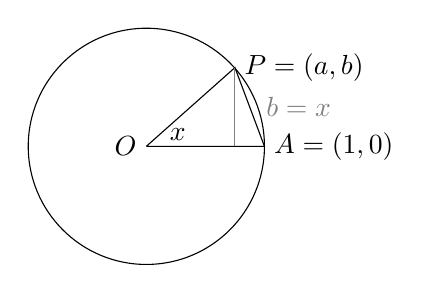
\begin{tikzpicture}[scale=.5]
	    \draw(0,0) circle (3);
	    \draw(0,0)node[left]{$O$}--(2.25,2)node[right]{$P=(a,b)$}--(3,0)node[right]{$A=(1,0)$}--(0,0);
	    \draw[gray](2.25,2)--(2.25,0);
	    \draw[gray](2.8,1)node[right]{$b=\sen x$};
	    \draw(.8,-.1)node[above]{$x$};
	\end{tikzpicture}
    \end{center}
    Asumiendo que el radio es $r=1$. Para $0<x<\frac{x}{2}$ tenemos el triangulo $OAP_t$ de tamaño de base $a=1$ y altura $b=\sen x$, es decir,
    $$Area(OAP_t) = \dfrac{1}{2}ab = \dfrac{\sen x}{2}$$
    Luego el área del sector circular $OAP_s$ es
    $$Area(OAP_s) = \dfrac{x}{2\pi}\pi r^2 = \dfrac{x}{2}$$
    Ya que el área del triángulo $OAP_t$ es menor al área del sector $OAP_t$ tenemos,
    $$\dfrac{\sen x}{2}<\dfrac{x}{2} \quad \Longrightarrow \quad \sen x < x$$
    dado que $\sen(-x)=-\sen x$ para $0<x<\frac{\pi}{2}$ entonces 
$$\sen x < x \quad \Longrightarrow \quad -\sen x > -x \quad \Longrightarrow \quad |\sen x| < |x|$$
para $0<|x|<\frac{x}{2}$.\\\\
    
\end{enumerate}

\setcounter{section}{9}
\section{la integral para el área en coordenadas polares}

\begin{teo}
    Sea $R$ el conjunto radial de una función no negativa $f$ en un intervalo $[a,b]$, donde $0\leq b-a\leq 2\pi$, y se asume que $R$ es medible. Si $f^2$ es integrable en $[a,b]$ el área de $R$ esta dado por la integral
    $$a(R)= \dfrac{1}{2}\int_a^b f^2(\theta)\; d\theta$$

    Demostración.-\; Elegimos dos funciones escalonadas $s$ y $t$ que satisface
    $$0\leq s(\theta) \leq f(\theta)\leq t(\theta)$$
    Para todo $\theta$ en $[a,b]$, y denotamos $S$ y $T$ sus conjuntos radiales, respectivamente. Ya que $s\leq f\leq t$ en $[a,b]$, los conjuntos radiales satisfacen la relación de inclusión $S\subseteq R \subseteq T.$ Por lo tanto, por la propiedad monótona del área, tenemos $a(S)\leq a(R) \leq a(T).$ Pero $S$ y $T$ son conjuntos radiales de la función escalonada, así $a(S) = \dfrac{1}{2}\displaystyle\int_a^b s^2(\theta)\; d\theta$ y $a(T) = \dfrac{1}{2}\displaystyle\int_a^b t^2 (\theta)\; d\theta$. Entonces tenemos la inecuación 
    $$\int_a^b s^2(\theta)\; d\theta \leq 2a(R)\leq \int_a^b t^2(\theta)\; d\theta$$
    para todo función escalonada $s$ y $t$ que satisface $s\leq f\leq t$ en $[a,b]$. Donde $s^2$ y $t^2$ son funciones escalonadas arbitrarias que satisfacen $s^2\leq f^2 \leq t^2$ en $[a,b]$, se sigue $f^2$ es integrable, y tenemos $2a(R)=\displaystyle\int_a^b f^2(\theta)\; d\theta$. Esto prueba el teorema.\\\\
\end{teo}


\section{Ejercicios}

En cada uno de los ejercicios 1 al 4, demostrar que el conjunto de puntos cuyas coordenadas rectangulares $(x,y)$ satisfacen la ecuación cartesiana dada, es igual al conjunto de todos los puntos cuyas coordenadas polares $(r,\theta)$ satisfacen la correspondiente ecuación polar.
\begin{enumerate}[ \bfseries 1.]

    %----------1.
    \item $(x-1)^2 + y^2 = 1;\quad r=2\cos \theta, \; cos \theta$.\\\\
	Respuesta.-\; Sea $x = r\cos \theta$ y $y=r\sen \theta$ entonces
	$$\begin{array}{rcr}
	    (x-1)^2 + y^2 = 1 &\Longrightarrow & (r\cos \theta - 1)^2 + r^2 \sen^2 \theta = 1\\
	    &\Longrightarrow & r^2 \cos^2 \theta - 2r \cos \theta  + 1 + r^2\sen^2 \theta = 1\\
	    &\Longrightarrow & r^2(\cos^2 \theta + \sen^2 \theta) - 2r\cos \theta = 0\\
	    &\Longrightarrow & r = 2\cos \theta\\
	\end{array}$$
	Donde $\cos \theta > 0$ entonces $r>0$.\\\\

    %----------2.
    \item $x^2 + y^2 - x = \sqrt{x^2 + y^2};\quad r=1+\cos \theta$.\\\\
	Respuesta.-\; Sea  $x = r\cos \theta$ y $y=r\sen \theta$ entonces
	$$\begin{array}{rcrcl}
	    x^2 + y^2 - x = \sqrt{x^2 + y^2}&\Longrightarrow&r^2\cos^2 \theta + r^2\sen^2 \theta&=&\sqrt{r^2\cos^2\theta + r^2\sen^2\theta}\\
	    &\Longrightarrow&r^2 - r\cos \theta&=&r\\
	    &\Longrightarrow&1+\cos \theta&=&r.\\\\
	\end{array}$$


    %----------3.
    \item $(x^2+y^2)^2 = x^2 - y^2,\; y^2 \leq x^2; \quad r=\sqrt{\cos 2\theta},\; \cos 2\theta \geq 0$\\\\
	Respuesta.-\; Sea $x = r\cos \theta$ y $y=r\sen \theta$ entonces
	$$\begin{array}{rcrcl}
	    (x^2+y^2)^2 = x^2 - y^2 &\Longrightarrow& (r^2 \cos^2 \theta + r^2 \sen^2 \theta)^2&=&r^2 \cos^2 \theta - r^2 \sen^2 \theta\\
				    &\Longrightarrow&r^4&=&r^2\cos(2\theta)\\
				    &\Longrightarrow&r^2&=&r^2 \cos(2\theta)\\
				    &\Longrightarrow&r&=&\sqrt{\cos(2\theta)}\\\\
	\end{array}$$
	Ya que $cos^2\theta - r^2 \sen^2 \theta$.\\\\


    %----------4.
    \item $(x^2+y^2) = |x^2 - y^2|;\quad r=\sqrt{|\cos 2\theta|}$\\\\
	Respuesta.-\; Sea $x = r\cos \theta$ y $y=r\sen \theta$ entonces
	$$\begin{array}{rcrcl}
	    (x^2+y^2) = |x^2 - y^2| &\Longrightarrow&(r^2\cos^2\theta + r^2\sen^2\theta)^2&=&|r^2\cos^2 \theta -r^2\sen^2\theta|\\
				    &\Longrightarrow&r^4&=&r^2|\cos(2\theta)|\\
				    &\Longrightarrow&r^2&=&|\cos(2\theta)|\\
				    &\Longrightarrow&&=&\sqrt{|\cos(2\theta)|}.\\\\
	\end{array}$$


En cada uno de los ejercicios del 5 al 15, trazar la gráfica de $f$ en coordenadas polares y calcular el área del conjunto radial de $f$ sobre el intervalo especificado. Se supondrá que cada conjunto es medible.\\


    %----------5.
    \item Espiral de Arquimedes: $f(\theta)=\theta,\quad 0\leq \theta \leq 2\pi$.\\\\
	Respuesta.-
	\begin{center}
	    \begin{tikzpicture}[scale=.55]
		\begin{polaraxis}[
		    xticklabels={,0,$\frac\pi6$,$\frac\pi3$,$\frac\pi2$,$\frac{2\pi}3$,$\frac{5\pi}6$,
		    $\pi$,$\frac{7\pi}6$,$\frac{4\pi}3$,$\frac{3\pi}2$,$\frac{5\pi}3$,$\frac{11\pi}6$}
		    ]
		    \addplot[mark = none, domain = 0:2*pi, data cs = polarrad, samples = 600, fill = gray!30,opacity=.5]{x};
		\end{polaraxis}
	    \end{tikzpicture}
	\end{center}
	$$\dfrac{1}{2}\int_0^{2\pi} \theta^2 \; d\theta = \dfrac{1}{2} \cdot \left(\dfrac{\theta^3}{3}\bigg|_0^{2\pi}\right) = \dfrac{1}{2}\cdot \dfrac{(2\pi)^3}{3} = \dfrac{4\pi^3}{3}$$\\\\

    %----------6.
    \item Circunferencia tangente al eje y: $f(\theta) = 2\cos \theta,\quad -\pi/2 \leq \theta\leq \pi/2$.\\\\
	Respuesta.-
	\begin{center}
	    \begin{tikzpicture}[scale=.55]
		\begin{polaraxis}[
		    xticklabels={,0,$\frac\pi6$,$\frac\pi3$,$\frac\pi2$,$\frac{2\pi}3$,$\frac{5\pi}6$,
		    $\pi$,$\frac{7\pi}6$,$\frac{4\pi}3$,$\frac{3\pi}2$,$\frac{5\pi}3$,$\frac{11\pi}6$}
		    ]
		    \addplot[mark = none, domain = -90:90, data cs = polar, samples = 360, fill = gray!30, opacity=.5]{2*cos(x)};
		\end{polaraxis}
	    \end{tikzpicture}
	\end{center}
	$$\begin{array}{rcl}
	    \dfrac{1}{2}\displaystyle\int_{-\pi/2}^{\pi/2} 4\cos^2 \theta \; d\theta&=&\displaystyle\int_{-\pi/2}^{\pi/2} (1-\sen^2\theta)\; d\theta\\\\
										    &=&2\displaystyle\int_{-\pi/2}^{\pi/2} 1 \; d\theta + \displaystyle\int_{-\pi/2}^{\pi/2} (1-2\sen^2\theta - 1)\; d\theta\\\\
										    &=&2\pi + \left(\displaystyle\int_{-\pi/2}^{\pi/2} \cos 2\theta \; d\theta\right)-\pi\\\\
										    &=&\pi +\dfrac{1}{2} \displaystyle\int_{-\pi/2}^{\pi/2} \cos \theta \; d\theta\\\\
										    &=&\dfrac{1}{2}\left(\sen \theta \bigg|_{-\pi}^\pi\right) + \pi\\\\
										    &=&\pi\\\\
	\end{array}$$
	\vspace{.5cm}

    %----------7.
    \item Dos circunferencias tangentes al eje $y$: $f(\theta) = 2|\cos \theta|,\quad 0\leq \theta \leq 2\pi$.\\\\
	Respuesta.-\; $$\dfrac{1}{2}\int_{0}^{2\pi} 4 \cos^2 \theta \; d\theta = 2\int_{0}^{2\pi} \left(\dfrac{1+\cos(2\theta)}{2}\right)\; d\theta = 2 \int_{0}^{2\pi} \dfrac{1}{2}\; d\theta +2 \int_0^{2\pi} \cos(2\theta)\; d \theta = 2\pi + 0 = 2\pi$$

    \begin{center}
	\begin{tikzpicture}[scale=.55]
	    \begin{polaraxis}[
		xticklabels={,0,$\frac\pi6$,$\frac\pi3$,$\frac\pi2$,$\frac{2\pi}3$,$\frac{5\pi}6$,
		$\pi$,$\frac{7\pi}6$,$\frac{4\pi}3$,$\frac{3\pi}2$,$\frac{5\pi}3$,$\frac{11\pi}6$}
		]
		\addplot[mark = none, domain = 0:360, data cs = polar,samples = 600, fill=gray!30,opacity=.5]{2*abs(cos(x))};
	    \end{polaraxis}
	\end{tikzpicture}
    \end{center}
    \vspace{.5cm}

    %----------8.
    \item Circunferencia tangente al eje $x$: $f(\theta) = 4\sen \theta, \quad 0\leq \theta \leq \pi$.\\\\
	Respuesta.-\; $$\dfrac{1}{2}\int_0^\pi 16\sen^2\theta \; d\theta = 8\int_0^\pi \sen^2 \theta \; d\theta = 8\left(\dfrac{\pi}{2}-\dfrac{1}{4} \sen 2\pi\right) = 4\pi$$

    \begin{center}
	\begin{tikzpicture}[scale=.55]
	    \begin{polaraxis}[
		xticklabels={,0,$\frac\pi6$,$\frac\pi3$,$\frac\pi2$,$\frac{2\pi}3$,$\frac{5\pi}6$,
		$\pi$,$\frac{7\pi}6$,$\frac{4\pi}3$,$\frac{3\pi}2$,$\frac{5\pi}3$,$\frac{11\pi}6$}
		]
		\addplot[mark = none, domain = 0:180, data cs = polar, samples = 600, fill=gray!30, opacity=.5]{4*sin(x)};
	    \end{polaraxis}
	\end{tikzpicture}
    \end{center}
    \vspace{.5cm}

    %----------9.
    \item Dos circunferencias tangentes al eje $x$: $f(\theta) = 4|\sen \theta|,\quad 0\leq \theta \leq 2\pi$.\\\\
	Respuesta.-\; $$\dfrac{1}{2}\int_0^\pi 16\sen^2\theta \; d\theta = 8\int_0^\pi \sen^2 \theta \; d\theta = 8\left(\dfrac{2\pi}{2}-\dfrac{1}{4} \sen 2\pi\right) = 8\pi$$

    \begin{center}
	\begin{tikzpicture}[scale=.55]
	    \begin{polaraxis}[
		xticklabels={,0,$\frac\pi6$,$\frac\pi3$,$\frac\pi2$,$\frac{2\pi}3$,$\frac{5\pi}6$,
		$\pi$,$\frac{7\pi}6$,$\frac{4\pi}3$,$\frac{3\pi}2$,$\frac{5\pi}3$,$\frac{11\pi}6$}
		]
		\addplot[mark = none, domain = 0:360, data cs = polar, samples = 600, fill=gray!30, opacity=.5]{4*abs(sin(x))};
	    \end{polaraxis}
	\end{tikzpicture}
    \end{center}
    \vspace{.5cm}

    %----------10.
    \item Pétalo de rosa: $f(\theta) = \sen 2\theta,\quad 0\leq \theta \leq \pi/2$.\\\\
	Respuesta.- 
	\begin{center}
	    \begin{tikzpicture}[scale=.55]
		\begin{polaraxis}[
		    xticklabels={,0,$\frac\pi6$,$\frac\pi3$,$\frac\pi2$,$\frac{2\pi}3$,$\frac{5\pi}6$,
		    $\pi$,$\frac{7\pi}6$,$\frac{4\pi}3$,$\frac{3\pi}2$,$\frac{5\pi}3$,$\frac{11\pi}6$}
		    ]
		    \addplot[mark = none, domain = 0:90, data cs = polar, samples = 600, fill=gray!30, opacity=.5]{sin(2*x)};
		\end{polaraxis}
	    \end{tikzpicture}
	\end{center}
	$$\dfrac{1}{2}\int_0^{\pi/2} \sen^2(2\theta)\; d\theta = \dfrac{1}{2\cdot 2}\int_{0\cdot 2}^{2 \cdot \pi/2} \sen^2\left(\dfrac{2\theta}{2}\right)\; d\theta = \dfrac{1}{4}\left[\dfrac{\pi}{2} + \dfrac{1}{4}\sen(2 \pi)\right] = \dfrac{\pi}{8}$$\\
	Se aplico el teorema 1.19 (dilatación o contracción del intervalo de integración) y la nota 2.4 respectivamente.\\\\

    %----------11.
    \item Rosa de cuatro hojas: $f(\theta) = |\sen 2\theta|,\quad 0\leq \theta \leq 2\pi$.\\\\
	Respuesta.-\;
	\begin{center}
	    \begin{tikzpicture}[scale=.55]
		\begin{polaraxis}[
		    xticklabels={,0,$\frac\pi6$,$\frac\pi3$,$\frac\pi2$,$\frac{2\pi}3$,$\frac{5\pi}6$,
		    $\pi$,$\frac{7\pi}6$,$\frac{4\pi}3$,$\frac{3\pi}2$,$\frac{5\pi}3$,$\frac{11\pi}6$}
		    ]
		    \addplot[mark = none, domain = 0:360, data cs = polar, samples = 600, fill=gray!30, opacity=.5]{abs(sin(2*x))};
		\end{polaraxis}
	    \end{tikzpicture}
	\end{center}
	$$\dfrac{1}{2}\int_0^{2\pi} \sen^2(2\theta)\; d\theta = \dfrac{1}{2\cdot 2}\int_{2\cdot 0}^{2\cdot 2 \pi}\sen^2\left(\dfrac{2\theta}{2}\right)\; d\theta = \dfrac{1}{4}\left[\dfrac{4\pi}{2} + \dfrac{1}{4}\sen(2\cdot 4\pi)\right] = \dfrac{\pi}{2}$$\\\\

    %----------12.
    \item Ocho aplastado: $f(\theta) = \sqrt{|\cos \theta|}, \quad 0\leq \theta \leq 2\pi$.\\\\
	Respuesta.-\;
	\begin{center}
	    \begin{tikzpicture}[scale=.55]
		\begin{polaraxis}[
		    xticklabels={,0,$\frac\pi6$,$\frac\pi3$,$\frac\pi2$,$\frac{2\pi}3$,$\frac{5\pi}6$,
		    $\pi$,$\frac{7\pi}6$,$\frac{4\pi}3$,$\frac{3\pi}2$,$\frac{5\pi}3$,$\frac{11\pi}6$}
		    ]
		    \addplot[mark = none, domain = 0:360, data cs = polar, samples = 600, fill=gray!30, opacity=.5]{sqrt(abs(cos(x)))};
		\end{polaraxis}
	    \end{tikzpicture}
	\end{center}
	$$\begin{array}{rcl}
	    \displaystyle\dfrac{1}{2}\int_0^{2\pi} \left(\sqrt{|\cos \theta|}\right)^2\; d\theta&=&\displaystyle \dfrac{1}{2}\left(\int_0^{\frac{\pi}{2}} \cos \theta\; d\theta - \int_{\frac{\pi}{2}}^{\frac{3\pi}{2}}\cos \theta\; d \theta + \int_{\frac{3\pi}{2}}^{2\pi} \cos \theta\; d \theta\right)\\\\
												&=&\dfrac{1}{2}\left[\sen\dfrac{\pi}{2} - \left(\sen \dfrac{3\pi}{2} - \sen \dfrac{\pi}{2}\right)+\sen 2\pi - \sen \dfrac{3\pi}{2}\right]\\\\
												&=&\dfrac{1}{2}\left(1 + 1 + 1 + 0 + 1\right)\\\\
	    &=&2\\\\
	\end{array}$$
	Esto por la nota 2.2. y por hecho de que 
	$$|\cos \theta| = \left\{\begin{array}{rcl}
	    +&si&0\leq x \leq \dfrac{\pi}{2}\\\\
	    -&si&\dfrac{\pi}{2} < x \leq \dfrac{3\pi}{2}\\\\
	    +&si&\dfrac{3\pi}{2} < x \leq 2\pi \\
	\end{array}\right.$$
	\vspace{.5cm}

    %----------13.
    \item Trébol de cuatro hojas: $f(\theta) = \sqrt{|\cos 2\theta|}, \quad 0\leq \theta \leq 2\pi$.\\\\
	Respuesta.-\;
	\begin{center}
		\begin{tikzpicture}[scale=.55]
		\begin{polaraxis}[
		    xticklabels={,0,$\frac\pi6$,$\frac\pi3$,$\frac\pi2$,$\frac{2\pi}3$,$\frac{5\pi}6$,
		    $\pi$,$\frac{7\pi}6$,$\frac{4\pi}3$,$\frac{3\pi}2$,$\frac{5\pi}3$,$\frac{11\pi}6$}
		    ]
		    \addplot[mark = none, domain = 0:360, data cs = polar, samples = 600, fill=gray!30, opacity=.5]{sqrt(abs(cos(2*x)))};
		\end{polaraxis}
	    \end{tikzpicture}
	\end{center}
	$$\begin{array}{rcl}
	    \dfrac{1}{2}\int_0^{2\pi}\left(\sqrt{|\cos(2\theta)|}\right)^2\; d\theta&=&\dfrac{1}{2\cdot 2}\int_{0\cdot 2}^{2\pi\cdot 2} \bigg|\cos\dfrac{2\theta}{2}\bigg|\; d\theta\\\\
	    &=&\dfrac{1}{4} \int_0^{4\pi} |\cos \theta| \; d\theta\\\\
	    &=&\dfrac{1}{4}\left(\displaystyle \int_0^{\frac{\pi}{2}} \cos \theta\; d\theta - \int_{\frac{\pi}{2}}^{\frac{3\pi}{2}}\cos \theta\; d \theta + \int_{\frac{3\pi}{2}}^{2\pi} \cos \theta\; d \theta\right.\\\\
	    &+& \left. \displaystyle \int_{2\pi}^{\frac{5\pi}{2}} \cos \theta\; d\theta - \int_{\frac{5\pi}{2}}^{\frac{7\pi}{2}}\cos \theta\; d \theta + \int_{\frac{7\pi}{2}}^{4\pi} \cos \theta\; d \theta\right)\\\\
	    &=&\dfrac{1}{4}\left[\sen \dfrac{\pi}{2} - \left(\sen \dfrac{3\pi}{2} - \sen \dfrac{\pi}{2}\right) + \sen 2\pi - \sen \dfrac{3\pi}{2}\right. \\\\ 
	    &+&\left. \sen \dfrac{5\pi}{2}- \sen 2\pi - \left(\sen \dfrac{7\pi}{2} - \sen \dfrac{5\pi}{2}\right) + \sen 4\pi - \sen \dfrac{7\pi}{2}\right] \\\\
	    &=&\dfrac{1}{4}\left(1 + 1+1+0+1 +1+1+1+0+1\right)\\\\
	    &=&2\\\\
	\end{array}$$
	\vspace{.5cm}

    %----------14.
    \item Cardioide: $f(\theta) = 1+\cos \theta,\quad 0\leq \theta \leq 2\pi$.\\\\
	Respuesta.-\;
	\begin{center}
	    \begin{tikzpicture}[scale=.55]
		\begin{polaraxis}[
		    xticklabels={,0,$\frac\pi6$,$\frac\pi3$,$\frac\pi2$,$\frac{2\pi}3$,$\frac{5\pi}6$,
		    $\pi$,$\frac{7\pi}6$,$\frac{4\pi}3$,$\frac{3\pi}2$,$\frac{5\pi}3$,$\frac{11\pi}6$}
		    ]
		    \addplot[mark = none, domain = 0:360, data cs = polar, samples = 600, fill=gray!30, opacity=.5]{1+cos(x)};
		\end{polaraxis}
	    \end{tikzpicture}
	\end{center}
	$$\begin{array}{rcl}
	    \dfrac{1}{2}\displaystyle\int_0^{2\pi}(1+\cos \theta)^2\; d\theta&=&\dfrac{1}{2}\displaystyle\int_0^{2\pi}\left(1+2\cos \theta + \cos^2 \theta \right) \; d\theta\\\\
									     &=&\dfrac{1}{2}\left(2\pi + 2\sen 2\pi + \dfrac{2\pi}{2} + \dfrac{1}{4}\sen 4 \pi\right)\\\\
									     &=&\dfrac{3\pi}{2}\\\\
	\end{array}$$
	\vspace{.5cm}

    %----------15.
    \item Caracol: $f(\theta) = 2 + \cos \theta,\quad 0\leq \theta \leq 2\pi$.\\\\
	Respuesta.-\;
	\begin{center}
	    \begin{tikzpicture}[scale=.55]
		\begin{polaraxis}[
		    xticklabels={,0,$\frac\pi6$,$\frac\pi3$,$\frac\pi2$,$\frac{2\pi}3$,$\frac{5\pi}6$,
		    $\pi$,$\frac{7\pi}6$,$\frac{4\pi}3$,$\frac{3\pi}2$,$\frac{5\pi}3$,$\frac{11\pi}6$}
		    ]
		    \addplot[mark = none, domain = 0:360, data cs = polar, samples = 600, fill=gray!30, opacity=.5]{2+cos(x)};
		\end{polaraxis}
	    \end{tikzpicture}
	\end{center}
	$$\begin{array}{rcl}
	    \dfrac{1}{2}\displaystyle\int_0^{2\pi}(2+\cos \theta)^2\; d\theta&=&\dfrac{1}{2}\displaystyle\int_0^{2\pi}\left(4 + 4\cos \theta + \cos^2 \theta \right) \; d\theta\\\\
									     &=&\dfrac{1}{2}\left(8\pi + 4\sen 2\pi + \dfrac{2\pi}{2} + \dfrac{1}{4}\sen 4 \pi\right)\\\\
									     &=&\dfrac{9\pi}{2}\\\\
	\end{array}$$
	\vspace{.5cm}

\end{enumerate}

\section{Aplicación de la integración al cálculo de volúmenes}
    \begin{enumerate}[\bfseries 1.]

	%----------1.
	\item \textbf{Propiedad de no negatividad.} Para cada conjunto $S$ de $\mathscr{A}$ se tiene $v(S)\geq 0$.

	%----------2.
	\item \textbf{Aditividad.} Si $S$ y $T$ pertenecen a $\mathscr{A}, S\cup T$ y  $S\cap T$ también pertenecen a $\mathscr{A}$, y se tiene $v(S\cup T) = v(S) + v(T) - v(S\cap T.)$

	%----------3.
	\item \textbf{Propiedad de la diferencia.} Si $S$ y $T$ pertenecen a  $\mathscr{A}$, siendo $S\subseteq T$, $T-S$ pertenece a $\mathscr{A}$ y se tiene $v(T-S)=v(T)-v(S)$.\\\\
	    Ya que $v(T-S)\geq 0$, implica también la siguiente propiedad monónota:
	    $$v(S)\leq v(T), \quad \mbox{para los conjuntos S y T en } \mathscr{A} \; con \; S\subseteq T.$$

	%----------4.
	\item \textbf{Principio de Cavalieri.}  Si $S$ y $T$ son dos sólidos de Cavalieri pertenecientes a $\mathscr{A}$ tales que $a(S\cap F)\leq a(T\cap F)$ para todo plano $F$ perpendicular a una recta dada, entonces $v(S)\leq v(T)$.

	%----------5.
	\item \textbf{Elección de escala.} Toda caja $B$ pertenece a $\mathscr{A}$. Si los lados o aristas de $B$ tienen longitudes $a,b$ y $c$, se tiene que $v(B)=abc$.

	%----------6.
	\item Todo conjunto convexo pertenece a $\mathscr{A}$. 

    \end{enumerate}

% -------------------- teorema 2.7 --------------------
\begin{teo}
    Sea $R$ un sólido de Cavalieri de $\mathscr{A}$ cuya función área seccional $a_R$, sea integrable en un intervalo $[a,b]$ y nula fuera del mismo. En tales condiciones el volumen de $R$ es igual a la integral del área seccional:
    $$v(R) = \int_a^b a_R(u)\; du$$\\
    Demostración.-\; Elijamos funciones escalonadas $s$ y $t$ tales que $s\leq a_R \leq t$ en $[a,b]$ y definamos $s$ y $t$ como nulas fuera de $[a,b]$. Para cada subintervalo de $[a,b]$ en el que $s$ sea constante, podemos imaginar un sólido cilíndrico construido de modo que su área seccional en este subintervalo tenga el mismo valor constante que $s$. La reunión de esos cilindros sobre los intervalos en los que $s$ es constante es un sólido $S$ cuyo volumen $v(S)$ es, por la aditividad, igual a la integral $\int_a^b s(u) \; du$. Del mismo modo, existe un sólido $T$, una reunión de cilindros, cuyo volumen $v(T)=\int_a^b t(u)\; du$. Pero $a_S(u) = s(u)\leq t(u)=a_r(u)$ para todo $u$ de $[a,b]$, de modo que el principio de Cavalieri implica que $v(S) \leq v(R)\leq v(T)$. En otras palabras, $v(R)$ satisface las desigualdades,
    $$\int_a^b s(u)\; du \leq v(R) \leq \int_a^b t(u)\; du.$$
    para todas las funciones escalonadas $s$ y $t$ que satisfacen $s\leq a_S \leq t$ en $[a,b]$. Puesto que $a_S$ es integrable en $[a,b]$, resulta que $v(R)=\int_a^b a_S(u)\; du$.
\end{teo}

\section{Ejercicios}


\begin{enumerate}[ \bfseries 1.]

    %---------------------1.
    \item Usa la integración para calculular el volumen de un cono circular recto engendrado haciendo girar alrededor del eje $x$ la gráfica de la función $f$ dada por $f(x)=xc$ en el intervalo $0\leq x\leq b$. Demostrar que el resultado es el producto de un tercio del área de la base por la altura del cono.\\\\
	Demostración.-\; Primero podemos ver que el área de un sección transversal de este sólido de revolución es $\pi c^2x^2$. Así, usando la ecuación del volumen de un sólido de Cavalieri tenemos,
	$$v(R)=\int_0^b \pi c^2x^2\; dx = \pi c^2 \dfrac{x^3}{3}\bigg|_0^b = \pi c^2 \dfrac{b^3}{3}$$
	Dado que el área de la base es $\pi (cb)^2$, y en vista de que $cb$ es el alto de $f(x)=cx$ a $x=b$ para luego girar alrededor del eje $x$, entonces tenemos
	$$V=\dfrac{1}{3}a(B)h = \pi c^2\dfrac{b^3}{3}$$\\

    En cada uno de los ejercicios del 2 al 7, calcular el volumen del sólido engendrado al girar el conjunto de ordenadas de la función $f$ sobre el intervalo indicado. Dibujar cada uno de los conjuntos de ordenadas.\\\\

    %---------------------2.
    \item $f(x)=\sqrt{x}\quad 0\leq x\leq 1$.\\\\
	Respuesta.-\; 

	\begin{center}
	    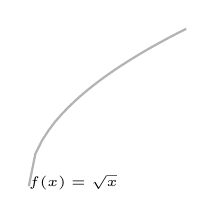
\begin{tikzpicture}[scale=2,draw opacity = 0.6]
		% abscisa y ordenada
		\tkzInit[xmax= 1,xmin=0, xstep = 1,ymax=1,ymin=0, ystep = 1]
		\tiny\tkzLabelXY[opacity=0.6,step=1, orig=false]
		% etiqueta x, f(x)
		\tkzDrawX[opacity=0.6,label=x,right=0.3]
		\tkzDrawY[opacity=0.6,label=f(x),below = -0.6]
		%dominio y función
		\draw [domain=0:1,thick,gray] plot(\x,{\x^(1/2)});
		\tkzText[opacity=0.6,above](0.5,1){\tiny $f(x)=\sqrt{x}$}
	    \end{tikzpicture}
	\end{center}

	Entonces calculando el volumen del sólido se tiene,
	$$V = \int_0^1 \pi \sqrt{x}^2 \; dx = \int_0^1 \pi x \; dx = \pi \dfrac{x^2}{2}\bigg|_0^1 = \dfrac{\pi}{2}.$$\\


    %---------------------3.
    \item $f(x)=x^{1/4},\quad 0\leq x\leq 1$.\\\\
	Respuesta.-\;

	\begin{center}
	    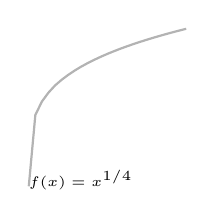
\begin{tikzpicture}[scale=2,draw opacity = 0.6]
		% abscisa y ordenada
		\tkzInit[xmax= 1,xmin=0, xstep = 1,ymax=1,ymin=0, ystep = 1]
		\tiny\tkzLabelXY[opacity=0.6,step=1, orig=false]
		% etiqueta x, f(x)
		\tkzDrawX[opacity=0.6,label=x,right=0.3]
		\tkzDrawY[opacity=0.6,label=f(x),below = -0.6]
		%dominio y función
		\draw [domain=0:1,thick,gray] plot(\x,{\x^(1/4)});
		\tkzText[opacity=0.6,above](0.5,1){\tiny $f(x)=x^{1/4}$}
	    \end{tikzpicture}
	\end{center}

	Luego calculamos el volumen del sólido de revolución.
	$$V = \int_0^1 \pi (x^{1/4})^2 = \int_0^1 \pi x^{1/2} =  \pi \dfrac{2x^{3/2}}{3}\bigg|_0^1 = \dfrac{2\pi}{3}$$\\


    %---------------------4.
    \item $f(x) = x^2,\quad -1\leq x\leq 2$.\\\\
	Respuesta.-\;

	\begin{center}
	    \begin{tikzpicture}[scale=1,draw opacity = 0.6]
		% abscisa y ordenada
		\tkzInit[xmax= 2,xmin=-1, xstep = 1,ymax=4,ymin=-1, ystep = 1]
		\tiny\tkzLabelXY[opacity=0.6,step=1, orig=false]
		% etiqueta x, f(x)
		\tkzDrawX[opacity=0.6,label=x,right=0.3]
		\tkzDrawY[opacity=0.6,label=f(x),below = -0.6]
		%dominio y función
		\draw [domain=-1:2,thick,gray] plot(\x,{abs(\x^2)});
		\tkzText[opacity=0.6,above](0.5,1){\tiny $f(x)=x^2$}
	    \end{tikzpicture}
	\end{center}

	Luego calculamos el volumen del sólido de revolución.
	$$V=\int_{-1}^2 \pi x^{2^2} \; dx = \int_{-1}^2 \pi x^{2} \; dx = \pi\dfrac{x^5}{5}\bigg|_{-1}^2 = \dfrac{33\pi}{5}.$$\\

    
    %---------------------5.
    \item $f(x) = \sen x, \quad 0\leq x\leq pi.$\\\\
	Respuesta.-\; 

	\begin{center}
	    \begin{tikzpicture}[scale=1,draw opacity = 0.6]
		% abscisa y ordenada
		\tkzInit[xmax= 3,xmin=0, xstep = 1,ymax=1,ymin=0, ystep = 1]
		\tiny\tkzLabelXY[opacity=0.6,step=1, orig=false]
		% etiqueta x, f(x)
		\tkzDrawX[opacity=0.6,label=x,right=0.3]
		\tkzDrawY[opacity=0.6,label=f(x),below = -0.6]
		%dominio y función
		\draw [domain=0:pi,thick,gray] plot(\x,{sin(deg(\x))});
		\tkzText[opacity=0.6,above](1.5,1){\tiny $f(x)=\sen x$}
	    \end{tikzpicture}
	\end{center}

	Calculamos el volumen del sólido de revolución.
	$$V=\int_0^\pi \pi \sen^2x\; dx = \dfrac{\pi}{2} \int_0^\pi [1-\cos(2x)]\; dx = \dfrac{\pi}{2}\pi = \dfrac{\pi^2}{2}.$$\\

    %---------------------6.
    \item $f(x) = \cos x, \quad 0\leq x \leq \pi/2$.\\\\
	Respuesta.-\; 

	\begin{center}
	    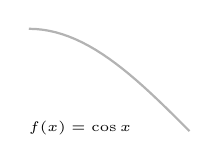
\begin{tikzpicture}[scale=1.3,draw opacity = 0.6]
		% abscisa y ordenada
		\tkzInit[xmax= 2,xmin=0, xstep = 1,ymax=1,ymin=0, ystep = 1]
		\tiny\tkzLabelXY[opacity=0.6,step=1, orig=false]
		% etiqueta x, f(x)
		\tkzDrawX[opacity=0.6,label=x,right=0.3]
		\tkzDrawY[opacity=0.6,label=f(x),below = -0.6]
		%dominio y función
		\draw [domain=0:pi/2,thick,gray] plot(\x,{cos(deg(\x))});
		\tkzText[opacity=0.6,above](1.5,1){\tiny $f(x)=\cos x$}
	    \end{tikzpicture}
	\end{center}

	Calculamos el volumen del sólido de revolución.
	$$V=\int_0^{\pi/2} = \pi \cos^2 x\; dx = \dfrac{\pi}{2} \int_0^{\pi/2} [1-\cos(2x)]\; dx = \dfrac{\pi^2}{4}.$$\\

    %---------------------7.
    \item $f(x) = \sen x + \cos x, \quad 0\leq x\leq \pi$.\\\\
	Respuesta.-\; 

	\begin{center}
	    \begin{tikzpicture}[scale=1.3,draw opacity = 0.6]
		% abscisa y ordenada
		\tkzInit[xmax= 3,xmin=0, xstep = 1,ymax=1,ymin=-1, ystep = 1]
		\tiny\tkzLabelXY[opacity=0.6,step=1, orig=false]
		% etiqueta x, f(x)
		\tkzDrawX[opacity=0.6,label=x,right=0.3]
		\tkzDrawY[opacity=0.6,label=f(x),below = -0.6]
		%dominio y función
		\draw [domain=0:pi,thick,gray] plot(\x,{sin(deg(\x))+cos(deg(\x))});
		\tkzText[opacity=0.6,above](2.5,1){\tiny $f(x)=\sen x + \cos x$}
	    \end{tikzpicture}
	\end{center}

	Calculamos el volumen del sólido de revolución.
	$$\begin{array}{rcl}
	    V&=&\int_0^\pi \pi (\sen x + \cos x)^2 \; dx\\\\
	     &=& \pi\left(\int_0^\pi \sen^2 x \;dx + \int_0^\pi 2\sen x \cos x + \int_0^\pi \cos^2 x \; dx\right)\\\\
	     &=& \pi \left(\dfrac{\pi}{2}+0+\dfrac{\pi}{2}\right)\\\\
	     &=& \pi^2.
	\end{array}$$

    En cada uno de los ejercicios 8 al 11, dibujar la región entre las gráficas de $f$ y $g$ y calcular el volumen del sólido obtenido al girar dicha región alrededor del eje $x$.\\\\

    %---------------------8.
    \item $f(x) = \sqrt{x},\quad g(x)=1,\quad 0\leq x\leq 1$.\\\\
	Respuesta.-\;

	\begin{center}
	    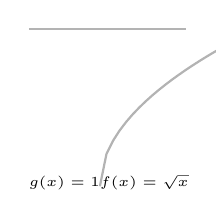
\begin{tikzpicture}[scale=2,draw opacity = 0.6]
		% abscisa y ordenada
		\tkzInit[xmax= 1,xmin=0, xstep = 1,ymax=1, ymin=0, ystep = 1]
		\tiny\tkzLabelXY[opacity=0.6,step=1, orig=false]
		% etiqueta x, f(x)
		\tkzDrawX[opacity=0.6,label=x,right=0.3]
		\tkzDrawY[opacity=0.6,label=f(x),below = -0.6]
		%dominio y función
		\draw [domain=0:1,thick,gray] plot(\x,{1});
		\tkzText[opacity=0.6,above](0.5,1){\tiny $g(x)=1$}
		\draw [domain=0:1,thick,gray] plot(\x,{sqrt(\x)});
		\tkzText[opacity=0.6,above](0.7,.4){\tiny $f(x)=\sqrt{x}$}
	    \end{tikzpicture}
	\end{center}

	Luego calculamos el volumen del sólido de revolución de la siguiente manera,
	$$V = \pi\int_0^1 (1^2 - \sqrt{x}^2)\; dx = \pi\int_0^1 (1-x)\; dx = \pi - \dfrac{\pi}{2} = \dfrac{\pi}{2}$$\\

    %---------------------9.
    \item $f(x)=\sqrt{x},\quad g(x)=x^2,\quad 0\leq x\leq 1$.\\\\
	Respuesta.-\;

	\begin{center}
	    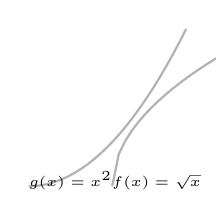
\begin{tikzpicture}[scale=2,draw opacity = 0.6]
		% abscisa y ordenada
		\tkzInit[xmax= 1,xmin=0, xstep = 1,ymax=1, ymin=0, ystep = 1]
		\tiny\tkzLabelXY[opacity=0.6,step=1, orig=false]
		% etiqueta x, f(x)
		\tkzDrawX[opacity=0.6,label=x,right=0.3]
		\tkzDrawY[opacity=0.6,label=f(x),below = -0.6]
		%dominio y función
		\draw [domain=0:1,thick,gray] plot(\x,{\x^2});
		\tkzText[opacity=0.6,above](1,.4){\tiny $g(x)=x^2$}
		\draw [domain=0:1,thick,gray] plot(\x,{sqrt(\x)});
		\tkzText[opacity=0.6,above](0.4,.8){\tiny $f(x)=\sqrt{x}$}
	    \end{tikzpicture}
	\end{center}

	Luego calculamos el volumen del sólido de revolución de la siguiente manera,
	$$V = \pi\int_0^1 (\sqrt{x}-x^{2^2})\; dx = \pi \int_0^1 (x-x^4)\; dx = \pi\left(\frac{1}{2}-\dfrac{1}{5}\right) = \dfrac{3\pi}{10}.$$\\

    %---------------------10.
    \item $f(x) = \sen x, \quad g(x)=\cos x,\quad 0\leq x \leq \pi/4$.\\\\
	Respuesta.-\;

	\begin{center}
	    \begin{tikzpicture}[scale=2,draw opacity = 0.6]
		% abscisa y ordenada
		\tkzInit[xmax= 1,xmin=0, xstep = 1,ymax=1, ymin=0, ystep = 1]
		\tiny\tkzLabelXY[opacity=0.6,step=1, orig=false]
		% etiqueta x, f(x)
		\tkzDrawX[opacity=0.6,label=x,right=0.3]
		\tkzDrawY[opacity=0.6,label=f(x),below = -0.6]
		%dominio y función
		\draw [domain=0:pi/4,thick,gray] plot(\x,{sin(deg(\x))});
		\tkzText[opacity=0.6,above](1,.4){\tiny $f(x)=\sen x$}
		\draw [domain=0:pi/4,thick,gray] plot(\x,{cos(deg(\x))});
		\tkzText[opacity=0.6,above](0.4,1){\tiny $g(x)=\cos x$}
	    \end{tikzpicture}
	\end{center}

	Luego calculamos el volumen del sólido de revolución de la siguiente manera,
	$$V=\pi\int_0^{\pi/4} (\cos^2 x - \sen^2 x)\; dx = \pi\int_0^{\pi/4} \cos(2x)\; dx = \dfrac{\pi}{2}\int_0^{\pi/2}\cos x\; dx = \dfrac{\pi}{2}.$$\\


    %---------------------11.
    \item $f(x) = \sqrt{4-x^2},\quad g(x)=1,\quad 0\leq x \leq \sqrt{3}$.\\\\
	Respuesta.-\;

	\begin{center}
	    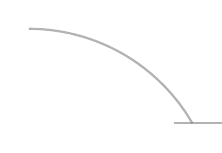
\begin{tikzpicture}[scale=1.2,draw opacity = 0.6]
		% abscisa y ordenada
		\tkzInit[xmax= 2,xmin=0, xstep = 1,ymax=2, ymin=0, ystep = 1]
		\tiny\tkzLabelXY[opacity=0.6,step=1, orig=false]
		% etiqueta x, f(x)
		\tkzDrawX[opacity=0.6,label=x,right=0.3]
		\tkzDrawY[opacity=0.6,label=f(x),below = -0.6]
		%dominio y función
		\draw [domain=0:3^(1/2),thick,gray] plot(\x,{(4-abs(\x^2))^(1/2)});
		\tkzText[opacity=0.6,above](1,1.9){\tiny $f(x)=\sqrt{4-x^2}$}
		\draw [domain=0:3^(1/2),thick,gray] plot(\x,{1});
		\tkzText[opacity=0.6,above](0.4,.7){\tiny $g(x)=1$}
	    \end{tikzpicture}
	\end{center}

	Luego calculamos el volumen del sólido de revolución de la siguiente manera,
	$$V = \pi\int_0^{\sqrt{3}}(4-x^2-1)\; dx = 3\pi \int_0^{\sqrt{3}}\; dx - \pi\int_0^{\sqrt{3}} x^2\; dx = 3\pi \sqrt{3} - \pi\sqrt{3} = 2 \pi \sqrt{3} .$$\\

    %---------------------12.
    \item Dibujar el gráfico de $f(x) = \sqrt{x}$ y $g(x)=x/2$ sobre el intervalo $[0,2]$. Encuentre un número $t$, $1<t<2$, de modo que la región entre los gráficos de $f$ y $g$ sobre el intervalo $[0,t]$ gira alrededor del eje $x$, engendra un sólido de revolución cuyo volumen es igual a $\pi t^3/3$.\\\\
	Respuesta.-\; El volumen del sólido de revolución generado por la región entre los gráficos $f$ y $g$ en el intervalo $[0,t]$ es,
	$$V=\pi\int_0^t \left(x-\dfrac{x^2}{4}\right)\; dx$$
	Así, 
	$$\dfrac{\pi t^2}{3} = \int_0^t \left(x-\dfrac{x^2}{4}\right)\; dx \;\Longrightarrow \; \dfrac{t^3}{3}=\dfrac{x^2}{2}\bigg|_0^t - \dfrac{x^3}{12}\bigg|_0^t \; \Longrightarrow \; \dfrac{t^3}{3} = \dfrac{t^2}{2} - \dfrac{t^3}{12} \; \Longrightarrow \; 4t^3 = 6t^2 - t^3 \; \Longrightarrow \; t=\dfrac{6}{5}.$$\\

    %---------------------13.
    \item ¿Qué volumen de material se quita de una esfera de radio $2r$ cuando se atraviesa con un taladro, formando un agujero centrado de radio $r$?.\\\\
	Respuesta.-\; Primero, el volumen de una esfera de radio $2r$ es dado por,
	$$V_S = \dfrac{4}{3}\pi(2r)^3 = \dfrac{32}{3}\pi r^3$$
	entonces, el volumen de una esfera con un agujero centrado es el volumen del sólido de revolución generado por la región entre $$f(x) = \sqrt{4r^2 - x^2}\quad \mbox{y} \quad g(x)=r \quad \mbox{para}\quad -\sqrt{3}r \; \mbox{hasta} \; \sqrt{3}r.$$ 
	Denotemos en volumen por $V_T$ de donde tenemos,
	$$\begin{array}{rcl}
	    V_T&=&\pi \left[\int_{-\sqrt{3}r}^{\sqrt{3}r}(4r^2-x^2 - r^2)\; dx\right]\\\\
	       &=&\pi \left[\int_{-\sqrt{3}r}^{\sqrt{3}r} (3r^2 - x^2)\; dx\right]\\\\
	       &=&4\sqrt{3}\pi r^3\\\\
	\end{array}$$
	Por lo tanto, el volumen de material que se quita de una esfera cuando se atraviesa con un taladro es,
	$$V_S - V_T = \dfrac{32}{3}\pi r^2.$$\\

    %---------------------14.
    \item Un servilletero se obtiene practicando un agujero cilíndrico en una esfera de modo que el eje de aquél pase por el centro de ésta. Si la longitud del agujero es $2h$, demostrar que el volumen del servilletero es $\pi ah^3$, siendo $a$ un número racional.\\\\
	Demostración.-\; Sea $r_s$ el radio de la esfera y $r_c$ el radio del agujero cilíndrico. Entonces el volumen del anillo es el volumen del sólido de revolución formado al rotación el área entre las funciones 
	$$f(x) = \sqrt{r_s^2 - x^2}, \quad g(x)=r_c,\quad -h\leq x\leq h$$
	sobre el eje $x$. Dado que la longitud del agujero es $2h$, sabemos que $f(h)=g(h)$; por lo tanto $r_s^2 - h^2 = r_c^2 \; \Longrightarrow \; r_s^2 - r_c^2 = h^2.$ Así se tiene,
	$$V = \pi\int_{-h}^h \left[\left(\sqrt{r_s^2 - x^2}\right)^2 - r_c^2\right]\; dx = \pi \int_{-h}^h (r_s^2 - r_c^2 -x^2)\; dx = \pi h^2 (2h) - \pi \dfrac{x^3}{3}\bigg|_{-h}^h = \dfrac{4}{3}\pi h^3 = \pi a h^3$$.\\

    %---------------------15.
    \item Un sólido tiene una base circular de radio $2$. Cada sección producida por un plano perpendicular a un diámetro fijo es un triángulo equilátero. Calcular el volumen del sólido.\\\\
	Demostración.-\; Podemos describir la mitad superior de la base circular del sólido mediante la ecuación
	$$f(x)=\sqrt{4-x^2}$$
	de donde, la longitud de la base de cualquier sección transversal triangular equilátera es,
	$$2\sqrt{4-x^2}\quad -2\leq x \leq 2$$
	Como estos son triángulos equiláteros, con lado de longitud $2\sqrt{4-x^2}$, el área es dada por 
	$$a(x) = \sqrt{3}(4-x^2)$$
	Por lo tanto, calculando el volumen se tiene,
	$$\begin{array}{rcl}
	    V&=&\sqrt{3}(4-x^2)\; dx\\\\
	     &=&3\sqrt{3}(4) - \sqrt{3}\left(\dfrac{x^3}{3}\bigg|_{-2}^2\right)\\\\
	     &=&16\sqrt{3} - \dfrac{16}{3}\sqrt{3}\\\\
	     &=&\dfrac{32\sqrt{3}}{3}\\\\
	\end{array}$$
	\vspace{0.5cm}

    %---------------------16.
    \item las secciones transversales de un sólido son cuadrados perpendiculares al eje $x$ con sus centros en el eje. Si el cuadrado cortado en $x$ tiene arista $2x^2$, encuentra el volumen del sólido entre $x = 0$ y $x = a$. Haz un dibujo.
	El área de las secciones transversales son dados por,
	$$A(x) = (2x^2)^2 = 4x^4$$
	Así, el volumen del sólido para $0\leq x \leq a$ será,
	$$V=\int_0^a 4x^4\; dx = \dfrac{4}{5}a^5.$$\\

    %---------------------17.
    \item Hallar el volumen de un sólido cuya sección transversal, por un plano perpendicular al eje $x$ tiene de área $ax^2+bx+c$ para $x$ del intervalo $0\leq x\leq h$. Expresar el volumen en términos de áreas $B_1,\; M$ y $B_2$ de la sección transversal correspondiente a $x=0$, $x=h/2$ y $x=h$, respectivamente.. La fórmula que resulta se conoce como fórmula del prismatoide.\\\\
	Respuesta.-\; Ya que el área de la sección transversal en $x$ está dada por $ax^2+bx+c$, tenemos,
	$$\begin{array}{rcl}
	    B_i&=&c\\\\
	      M&=&\dfrac{ah^2}{4}+\dfrac{bh}{2}+c\\\\
	    B_2&=&ah^2 + bh + c\\\\
	\end{array}$$
	entonces, calculamos el volumen de la siguiente manera.
	$$\begin{array}{rcl}
	    V&=&\displaystyle\int_0^h (ax^2 + bx + c)\; dx\\\\
	     &=&\dfrac{ah^3}{3} + \dfrac{bh^2}{2} + ch\\\\
	     &=&\dfrac{h}{6}(2ah^2 + 3bh + 6c)\\\\
	     &=&\dfrac{h}{6} (B_1 + 4M + B_2)\\\\
	\end{array}$$
	\vspace{0.5cm}

    %---------------------18.
    \item Dibujar un esquema de la región en el plano $xy$ formada por todos los puntos $(x,y)$ que satisfacen las desigualdades simultaneas $0\leq x\leq 2,$  $\frac{1}{4}x^2 \leq y \leq 1$. Calcular el volumen del solido obtenido haciendo girar esta región: a) alrededor del eje $x$; b) alrededor del eje $y$ c) alrededor de la vertical que pasa por $(2,0)$; de la horizontal que pasa por $(0,1)$.\\\\
	Respuesta.-\; 

	\begin{center}
	    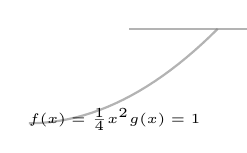
\begin{tikzpicture}[scale=1.2,draw opacity = 0.6]
		% abscisa y ordenada
		\tkzInit[xmax= 2,xmin=0, xstep = 1,ymax=1.5, ymin=0, ystep = 1]
		\tiny\tkzLabelXY[opacity=0.6,step=1, orig=false]
		% etiqueta x, f(x)
		\tkzDrawX[opacity=0.6,label=x,right=0.3]
		\tkzDrawY[opacity=0.6,label=f(x),below = -0.6]
		%dominio y función
		\draw [domain=0:2,thick,gray] plot(\x,{1/4*\x^2});
		\tkzText[opacity=0.6,above](1.9,.2){\tiny $f(x)=\frac{1}{4} x^2$}
		\draw [domain=0: 2,thick,gray] plot(\x,{1});
		\tkzText[opacity=0.6,above](1,1.2){\tiny $g(x)=1$}
	    \end{tikzpicture}
	\end{center}

	Para el inciso $a)$, calculamos el volumen al girar sobre el eje de la siguiente manera
	$$V=\pi\int_0^2 \left[1-\left(\dfrac{x^2}{4}\right)^2\right]\; dx = 2\pi-\dfrac{\pi}{16}\int_0^2 x^4 \; dx = \dfrac{8\pi}{5}$$

	Para el inciso $b)$ encontraremos una ecuación para $\dfrac{1}{4}x^2$ en términos de $x$, como sigue
	$$y=\dfrac{1}{4}\; dx,\quad \Longrightarrow \; |x|=2\sqrt{y}$$
	entonces calculamos el volumen de la siguiente manera al girar alrededor del eje de la siguiente manera,

	$$V = \pi\int_0^1 (2\sqrt{y})^2\; dy = 2\pi$$

	Para el inciso $c)$, calculamos el volumen de la siguiente manera al girar alrededor de la línea vertical de la $x=2$ de la siguiente manera.
	$$\begin{array}{rcl}
	    V &=& \pi\displaystyle\int_0^1 4 \;dy \\\\
	    &=&4\pi -\pi\displaystyle\int_0^1 (4-8\sqrt{y}+4y)\; dx\\\\
	    &=&\dfrac{p\pi}{3}\\\\
	\end{array}$$

	Y por último para el inciso d) calculamos el volumen de la siguiente manera al girar alrededor de la linea horizontal de la $y=1$ de la siguiente manera.\\\\
	$$V=\int_0^2\left(\dfrac{1}{4}x^2 - 1\right)^2 \; dx = \dfrac{16\pi}{15}.$$\\\\

\end{enumerate}


\section{Aplicación de la integración al concepto del trabajo}

%---------------------Propiedades fundamentales del trabajo
    \begin{prop}[Propiedades fundamentales del trabajo]
	Designemos con $W_a(f)$ el trabajo realizado por una función fuerza $f$ al mover una partícula desde $a$ hasta $b$. Entonces el trabajo tiene las siguientes propiedades:
	\begin{enumerate}[\bfseries 1.]

	    %----------1.
	    \item Propiedad aditiva. Si $a<c<b$. Entonces $W_a^c(f) + W_c^b(f)$.

	    %----------2.
	    \item Propiedad monótona. Si $f\leq g$ en $[a,b]$, entonces $W_a^b (f) \leq W_a^b(g)$. Esto es una mayor fuerza realiza un mayor trabajo.

	    %----------3.
	    \item Fórmula elemental. Si $f$ es constante, $f(x)=c$ para todo $x$ in el intervalo abierto $(a,b)$, entones $W_a^b(f) = c \cdot (b-a)$.\\\\

	\end{enumerate}

	La propiedad aditiva puede extenderse por inducción para cualquier número infinito del intervalo.\\
	Esto es, si $a=x_0<x_1<\ldots<x_n = b,$ tenemos,
	$$W_a^b(f) = \sum\limits_{k=1}^n W_k$$
	Donde $W_k$  es el trabajo realizado por $f$ desde $x_{k-1}$ a $x_k$. En particular, si la fuerza es una función escalonada $s$ que toma un valor constante $s_k$ en el intervalo abierto $(x_{k-1}-x_k)$ la propiedad 3 establece que $W_k = s_k\cdot (x_k-x_{k-1})$, con lo que 
	$$W_a^b (s) = \sum_{k=0} s_k \cdot (x_k-x_{k-1}) = \int_a^b s(x)\; dx$$
	Así pues, para funciones escalonadas, el trabajo se expresa como una integral. Es fácil demostrar que esto es cierto en casos más generales.
    \end{prop}

%--------------------- Teorema 2.8
\begin{teo}
    Supóngase que el trabajo fue definido para una clase de funciones fuerza $f$ de modo que satisface las propiedades 1, 2, 3. Entonces el trabajo efectuado por una función fuerza integrable $f$ al mover una partícula desde $a$ hasta $b$ es igual a la integral de $f$.
    $$W_a^b (f) = \int_a^b f(x)\; dx.$$
    Demostración.-\; Sean $s$ y $t$ dos funciones escalonadas que satisfacen $s\leq f\leq t$ en $[a,b]$. La propiedad del trabajo establece que $W_a^b (s) \leq W_a^b(f) \leq W_a^b (t)$. Pero $W_a^b (s) = \int_a^b s(x)$ y $W_a^b (t) = \int_a^b t(x) \;dx $ de modo que el número $W_a^b (f)$ satisface las desigualdades
    $$\int_a^b s(x)\; dx \leq W_a^b (f) \leq \int_a^b t(x)\; dx$$
    para todas las funciones escalonadas $s$ y $t$ que satisfacen $s\leq f\leq t$ en $[a,b]$. Puesto que $f$ es integrable en $[a,b]$, resulta que $W_a^b (f) = \int_a^b f(x)\; dx.$
\end{teo}


\section{Ejercicios}
En los ejercicios 1 y 2 se supone que la fuerza que actúa sobre el resorte obedece la ley de Hooke.\\\\

\begin{enumerate}[ \bfseries 1.]

    %----------1.
    \item Si una fuerza de 10 libras alarga un muelle elástico 1 pulgada, ¿qué trabajo se realiza al alargar el muelle 1 pie?.\\\\
	Respuesta.-\; Sea 1 pulgada = $\dfrac{1}{12}$ pie, entonces $f\left(\dfrac{1}{12}\right) = 10$ por lo tanto $c=120$, luego 
	$$W=\int_0^1 120x\; dx = \dfrac{}{}\bigg|_0^1 = 60\; pies-libra$$\\

    %----------2.
    \item Un muelle tiene normalmente la longitud de 1 metro. Una fuerza de 100 newtons la comprime hasta $0.9$ m. ¿Cuántos joules de trabajo se precisan para comprimirlo hasta la mitad de su longitud normal? ¿Cuál es la longitud del muelle cuando ya se han realizado 20 joules de trabajo?.\\\\
	Respuesta.-\; Sea $f(100) = 100c = 0.1\; Longrightarrow \; c=1000$
	Luego calculamos cuanto trabajo es requerido para comprimir el muelle 0.5 metros,
	$$W = \int_0^5 1000x\; dx = 1000\left(\dfrac{x^2}{2}\bigg|_0^5\right) = 125 joules.$$
	Como nos dan una cantidad de trabajo (20 loules) de donde resolveremos par un distacia a. Para la fórmula de trabajo tenemos,
	$$\int_0^a 1000x\; dx \; \Longrightarrow \; a=0.2\;m$$
	Dado que su longitud inicial es 1 m, tenemos que la longitud del resorte cuando se comprime es igual a $1m-0.2m = 0.8m$.\\\\

    %----------3.
    \item Una partícula se mueve a lo largo del eje $x$ mediante una fuerza impulsora $f(x)=3x^2+4x$ newtons. Calcular cuántos joules de trabajo se realizan con esa fuera para trasladar la particular a) desde $x=0$ hasta $x=7$; b) desde $x=2m$ hasta $x=7m$.\\\\
	Respuesta.-\; a) Usando la fórmula de trabajo entonces,
	$$W=\int_0^7 (3x^2+4x)\; dx = x^3\bigg|_0^7 + 2x^2\bigg|_0^7 = = 343+98=441\; joules.$$
	b) Usando la fórmula de trabajo entonces,
	$$W=\int_2^7 (3x^2+4x)\; dx = (x^3 + 2x^2)\bigg|_2^7 = = 441 - 16 = 425\; joules.$$\\\\


    %----------4.
    \item Una partícula se mueve a lo largo del eje $x$ mediante una fuerza impulsadora dada por $f(x)=ax^2+bx$ dinas. Calcular $a$ y $b$ de modo que se precisen $900$ ergs de trabajo para desplazar la partícula $10cm$ a partir del origen, si la fuerza es de $65$ dinas cuando $x=4cm$.\\\\
	Respuesta.-\; Dado $f(5) = 65$, entonces,
	$$f(5) = 25a + 5b = 65 \; \Longrightarrow \; b=13-5a$$
	luego, ya que $900$ ergs de trabajo son requeridos para mover una partícula de $10cm$, tenemos que,
	$$\begin{array}{rcl}
	    \displaystyle\int_0^{10}&\Longrightarrow&\dfrac{ax^3}{3}\bigg|0^{10} + \dfrac{bx^2}{2}\bigg|_0^{10} = 900\\\\
				    &\Longrightarrow&\left(\dfrac{1000}{3}\right)a + 50b = 900\\\\
				    &\Longrightarrow&\left(\dfrac{1000}{3}\right)a + 650 - 150a=900\\\\
	    &\Longrightarrow&a=3, \qquad b=-2\\\\
	\end{array}$$

    %----------5.
    \item Un cable de $50$ pies de longitud y $4$ libras de peso por pie pende de un torno. Calcular el trabajo realizado al enrollar $25$ pies de cable. No considerar más fuerzas que la gravedad.\\\\
	Respuesta.-\; La función fuerza es $f(x)=200-4x$, es decir, el peso total del cable menos $4$ libras por pie, cuando enrollaos el cable. Se sigue que,
	$$W = \int_0^{25} (200-4x)\; dx = 200\cdot 25 - 2\cdot 625 = 3750\; libras-pie.$$\\

    %----------6.
    \item Resolver el ejercicio 5 si se cuelga un peso de $50$ libras en el extremo del cable.\\\\
	Respuesta.-\; Dado que se tiene un peso de $50$ libras en el extremo del cable, la función de fuerza ahora está dada por $f(x) = 250-4x$. Entonces, el trabajo requerido es,
	$$W = \int_0^{25} (250-4x)\; dx = 6250-1250 = 5000\; libras-pie.$$\\

    %----------7.
    \item Un peso de $150$ libras se fija en un extremo de una cadena cuyo peso es de $2$ libras por pie. Inicialmente el peso se suspende con $10$ pies de cadena sobre el borde de un edificio de $100$ pies de altura. Considerando sólo la fuerza de gravedad, calcular el trabajo realizado cuando el peso se baja hasta una posición de $10$ pies sobre el suelo.\\\\
	Respuesta.-\; Dado que el edificio mide $100$ pies y el extremo cuelga inicialmente $10$ pies sobre el borde del edificio, comienza en una posición de $90$ pies sobre el suelo. Se baja a $10$ pies sobre el suelo. La fuerza de gravedad que actúa sobre la cadena es $f(x)=150+2x$, por lo que el trabajo realizado es 
	$$W = \int_{10}^{90}(150+2x)\; dx 0 150\cdot 80 + 90^2 - 10^2 = 2000 \; libras-pies.$$\\

    %----------8.
    \item En el ejercicio 7, suponer que la cadena sólo tiene $60$ pies de longitud y que el peso y la cadena se dejan caer al suelo, partiendo de la misma posición inicial que antes. Calcular el trabajo realizado por la fuerza de la gravedad cuando el peso alcanza el suelo.\\\\
	Respuesta.-\; Ahora tenemos una función de fuerza definida por partes: una parte mientras parte de la cadena aún está sobre el borde, y la otra parte una vez que toda la cadena está sobre el borde. Esta función es
	$$f(x)=\left\{\begin{array}{rcl}
		170+2x & para & 0\leq x\leq 50\\
		270 & para & 50\leq x\leq 90\\
	\end{array}\right.$$
	Así, el trabajo realizado es,
	$$W = \int_0^{50}(170+2x)\; dx + \int_{50}^{90} 270\; dx = 170\cdot 50 + 50^2 + 270\cdot(90-50) = 21800\; libras-pie.$$\\

    %----------9.
    \item Sea $V(q)$ el voltaje necesario para situar una carga $q$ en las placas de un condensador. El trabajo necesario para cargar un condensador desde $q=a$ hasta $q=b$ se define mediante la integral $\int_a^b V(q)\; dx$. Si el voltaje es proporcional a la carga, demostrar que el trabajo realizado para situar una carga $Q$ es un condensador descargado $\frac{1}{2}QV(Q)$.\\\\
	Demostración.-\; Ya que asumimos que el voltaje es proporcional a la carga, tenemos $V(q)=cq$ para alguna constante $c$, entonces,
	$$\begin{array}{rcl}
	    W&=&\displaystyle\int_a^b V(q)\; dq\\\\
	    &=&\displaystyle\int_a^b cq\; dq\\\\
	    &=&c\dfrac{q^2}{2}\bigg|_a^b\\\\
	    &=&\dfrac{1}{2}\left[cv(b)-cv(a)\right]\\\\
	    &=&\dfrac{1}{2}QV(Q)\\\\
	\end{array}$$
    
\end{enumerate}


\section{Valor medio de una función}

%-------------------- definición de valor medio de una función en un intervalo.
    \begin{def.}[Definición del valor medio de una función en un intervarlo]
	Si $f$ es integrable en un intervalo $[a,b]$, definimos $A(f)$, el valor medio de $f$ en $[a,b]$, por la siguiente fórmula
	$$A(f) = \dfrac{1}{b-a} \int_a^b f(x) \; dx$$\\
    Podemos ahora demostrar que ésta la fórmula es en realidad una extensión del concepto de media aritmética. Sea $f$ una función escalonada que es constante en cada uno de los subintervalos de $[a,b]$, obtenidos al dividirlo en $n$ partes iguales. En particular, sea $x_k=a+k(b-a)/n$ para $k=0,1,2,\ldots,n,$ y supongamos que $f(x)=f(x_k),$ si $x_{x-1}<x<x_k$. Entonces será $x_k - x_{k-1} = (b-a)/n$, con lo que se tiene
    $$\dfrac{1}{b-a}\int_a^b f(x)\; dx = \dfrac{1}{b-a}\sum_{k=0}^n f(x_k) \dfrac{b-a}{n} = \dfrac{1}{n} \sum_{k=1}^n f(x_k)$$
    Así pues, para funciones escalonadas, el promedio $A(f)$ coincide con la media aritmética de los valores $f(x_1),\ldots , f(x_k)$ tomados en los intervalos en los que la función es constante.
    
    \end{def.}

% --------------------- Definición de media ponderada.
    \begin{def.}[Definición del valor medio de una función en un intervarlo]
	$$A(f) = \dfrac{\int_a^b w(x)f(x)\; dx}{f_a^b w(x)\; dx}$$
    \end{def.}

% --------------------- Primer momento al rededor de 0 
    \begin{def.}[Primer momento al rededor de 0]
	$$\overline{x}=\dfrac{\int_0^b xp(x)\; dx}{\int_0^a p(x)\; dx} \; \mbox{para}\; p \; \mbox{llamada densidad de masa}.$$
    \end{def.}

%--------------------- Segundo momento al rededor de 0
    \begin{def.}[Segundo momento al rededor de 0 o momento de inercia]
	$$r^2=\dfrac{\int_0^b x^2p(x)\; dx}{\int_0^a p(x)\; dx} \; \mbox{para}\; p \; \mbox{llamada densidad de masa}.$$
    \end{def.}


\section{Ejercicios}

\begin{enumerate}[\bfseries 1.]

%-------------------- 1.
\item $f(x)=x^2,\quad a\leq x \leq b.$\\\\
    Respuesta.-\; $$A(f) = \dfrac{1}{b-a}\int_a^b x^2\; dx = \dfrac{1}{b-a} \cdot \dfrac{x^3}{3}\bigg|_a^b = \dfrac{1}{b-a}\cdot \dfrac{b^3 - a^3}{3}=\dfrac{b^3 - a^3}{3(b-a)} = \dfrac{b^2+2ba+a^2}{3}.$$\\

%-------------------- 2.
\item $f(x)=x^2+x^3, \quad 0\leq x \leq 1.$\\\\
    Respuesta.-\; $$A(f) = \dfrac{1}{1-0}\int_0^1 (x^2+x^3)\; dx = \dfrac{x^3}{3}\bigg|_0^1 + \dfrac{x^4}{4}\bigg|_0^1 = \dfrac{1}{3} + \dfrac{1}{4} = \dfrac{7}{12}.$$\\

%-------------------- 3.
\item $f(x)=x^{1/2},\quad 0\leq x \leq 4.$\\\\
    Respuesta.-\; $$A(f)=\dfrac{1}{4-0}\int_0^4 x^{1/2}\; dx = \dfrac{1}{4}\cdot \dfrac{2x^{3/2}}{3}\bigg|_0^4\; = \dfrac{4}{3}.$$\\

%-------------------- 4.
\item $f(x)=x^{1/3},\quad 1\leq x \leq 8.$\\\\
    Respuesta.-\; $$A(f) = \dfrac{1}{8-1}\int_1^8 x^{1/3}\; dx = \dfrac{1}{7}\cdot \dfrac{3x^{4/3}}{4}\bigg|_1^8 = \dfrac{48-3}{7} = \dfrac{45}{28}.$$\\ 

%-------------------- 5.
\item $f(x)=\sen x,\quad 0\leq x \leq \pi/2$.\\\\
    Respuesta.-\; $$A(f)=\dfrac{1}{\pi/2}\int_0^{\pi/2} \sen x\; dx = \dfrac{2}{\pi}\cdot (1-\cos \pi/2) = \dfrac{2}{\pi}.$$\\

%-------------------- 6.
\item $f(x)=\cos x,\quad -\pi/2\leq x \leq \pi/2.$\\\\
    Respuesta.-\; $$A(f)=\dfrac{1}{\pi/2 + \pi/2}\int_{-\pi/2}^{\pi/2} \cos x\; dx = \dfrac{1}{\pi}\cdot (\sen \pi/2 + \sen \pi/2) = \dfrac{2}{\pi}.$$\\

%-------------------- 7.
\item $f(x)=\sen 2x,\quad 0\leq x \leq \pi/2.$\\\\
    Respuesta.-\; $$A(f) = \dfrac{2}{\pi}\int_0^{\pi/2}\sen(2x)\; dx =  \dfrac{2}{2\pi}\int_{0\cdot 2}^{\frac{\pi}{2}\cdot 2}  \sen x\; dx = -\dfrac{1}{\pi}(1 -\cos \pi) = \dfrac{2}{\pi}$$.\\

%-------------------- 8.
\item $f(x)=\sen x \cos x,\quad 0\leq x \leq \pi/4.$\\\\
    Respuesta.-\; $$A(f)=\dfrac{4}{\pi}\int_0^{\pi/4}\sen x \cos x\; dx = \dfrac{2}{\pi}\int_0^{\pi/4}\sen(2x)\; dx = \dfrac{1}{\pi}\int_0^{\pi/2}\sen x\; dx = \dfrac{1}{\pi}\left(1-\cos \dfrac{\pi}{2}\right) = \dfrac{1}{\pi}.$$\\

%-------------------- 9.
\item $f(x)=\sen^2 x, \quad 0\leq x \leq \pi/2.$\\\\
    Respuesta.-\; $$A(f) = \dfrac{2}{\pi}\int_0^{\pi/2} \sen^2 x \; dx = \dfrac{1}{\pi}\int_0^{\pi/2} (1-\cos 2x)\; dx = \dfrac{1}{2} - \dfrac{1}{2\pi}\sen \pi = \dfrac{1}{2}.$$\\

%-------------------- 10.
\item $f(x)=\cos^2 x, \quad 0\leq x \leq pi.$\\\\
    Respuesta.-\; $$A(f) = \dfrac{1}{\pi}\int_0^{\pi}\cos^2 x\; dx = \dfrac{1}{2\pi}\int_0^\pi (1-\cos 2x)\; dx = \dfrac{1}{2\pi}\left(\pi + \dfrac{1}{2}\sen 2\pi\right) = \dfrac{1}{2}.$$\\

%-------------------- 11.
\item 
    \begin{enumerate}[\bfseries (a)]

	%----------(a)
	\item Si $f(x)=x^2$ para $0\leq x \leq a$, hallar un número $c$ que satisfaga $0<x<a$ y tal que $f(c)$ sea igual al promedio de $f$ en $[0,a].$\\\\
	    Respuesta.-\; $$\dfrac{1}{a}\int_0^a x^2\; dx = c^2 \Longrightarrow \dfrac{1}{a}\cdot \dfrac{x^3}{3}\bigg|_0^a = c^2 \Longrightarrow c = \dfrac{a}{\sqrt{3}}.$$\\

	%----------(b)
	\item Resolver la parte (a) si $f(x) = x^n$, siendo $n$ un entero positivo cualquiera.\\\\
	    Respuesta.-\; Generalizando el anterior ejercicio tenemos,
	    $$c^n = \frac{1}{a}\int_0^a x^n \; dx \Longrightarrow c = \dfrac{a}{(n+1)^{1/n}}.$$\\

    \end{enumerate}

%-------------------- 12.
\item Sea $f(x)=x^2$ para $0\leq x \leq 1$. El valor medio de $f$ en $[0,1]$ es $\frac{1}{3}$- Hallar una función peso no negativa $w$ tal que la media ponderada de $f$ en $[0,1]$, definida en 2.19 sea:\\\\
	    Respuesta.-\; Sabiendo que,
	    $$A(f)=\dfrac{\int_a^b w(x)f(x)\; dx}{\int_a^b w(x)\; dx}$$
	    entonces 

    \begin{enumerate}[\bfseries (a)]

	%----------(a)
	\item $\dfrac{1}{2}.$\\\\
	    Será $w(x)=x$ para que $A(f)=\dfrac{1}{2}.$ Como se verá a continuación.
	    $$A(f)=\dfrac{\int_a^b x\cdot x^2 \; dx}{\int_0^1 x\; dx}=\dfrac{\frac{1}{4}}{\frac{1}{2}}=\dfrac{1}{2}.$$\\

	%----------(b)
	\item $\dfrac{3}{5}.$\\\\
	    Sea $w(x)=x^2$, entonces
	    $$A(f)=\dfrac{\int_a^b x^2\cdot x^2}{\int_0^1 x^2\; dx}=\dfrac{\frac{1}{5}}{\frac{1}{3}}=\dfrac{3}{5}.$$\\

	%----------(c)
	\item $\dfrac{2}{3}$.\\\\
	    Sea $w(x)=x^3$, entonces
	    $$A(f)=\dfrac{\int_a^b x^3\cdot x^2}{\int_0^1 x^3\; dx}=\dfrac{\frac{1}{6}}{\frac{1}{4}}=\dfrac{2}{3}.$$\\

    \end{enumerate}

%-------------------- 13.
\item Sea $A(f)$ el promedio de $f$ en $[a,b]$. Demuestre que el promedio tiene las siguientes propiedades:
    \begin{enumerate}[\bfseries (a)]

	%----------(a)
	\item \textbf{Propiedad aditiva:} $A(f+g) = A(f)+A(g)$.\\\\
	    Demostración.-\; Sea $$A(f+g) = \dfrac{1}{b-a}\int_a^b f(x) + g(x) \; dx$$
	    entonces por la el teorema 1.17 (aditividad respecto al intervalo de integración) se tiene,
	    $$\dfrac{1}{b-a}\int_a^b f(x) + g(x) \; dx = \dfrac{1}{b-a}\int_a^b f(x)\; dx + \dfrac{1}{b-a}\int_a^b g(x)\; dx = A(f) + A(g)$$
	    así queda demostrado la propiedad aditiva del valor medio de una función.\\\\

	%----------(b)
	\item \textbf{Propiedad homogénea:} $A(cf)=c A(f)$ si $c$ es algún número real.\\\\
	    Demostración.-\; Sea $$A(cf)=\dfrac{1}{b-a}\int_a^b c[f(x)]\; dx$$
	    entonces por el teorema 1.16 (linealidad respecto al integrando) se tiene,
	    $$\dfrac{1}{b-a}\int_a^b c[f(x)]\; dx = c\left[\dfrac{1}{b-a}\int_a^b f(x)\; dx\right] = cA(f).$$\\

	%----------(c)
	\item \textbf{Propiedad monótona:} $A(f)\leq A(g)$ si $f\leq g$ en $[a,b]$.\\\\
	    Demostración.-\; dado que $f(x)\leq g(x)$ entonces por el teorema de comparación (teorema 1.20) obtenemos que,
	    $$\int_a^b f(x)\; dx \leq \int_a^b g(x)\; dx \; \Longrightarrow \; \dfrac{1}{b-a}\int_a^b f(x)\; dx\leq \dfrac{1}{b-a}\int_a^b g(x)\; dx \; \Longrightarrow \; A(f)\leq A(g).$$\\\\
    \end{enumerate}

%-------------------- 14.
\item ¿Cuáles de la propiedades del problema 13 son validas para las medias ponderadas definidas en 2.19?.\\\\
    Respuesta.-\; Para $A(f+g)$ tenemos,
    $$\begin{array}{rcl}
	A(f+g)&=&\dfrac{\int_a^b w(x)\left[f(x)+g(x)\right]\; dx}{\int_a^b w(x)\; dx}\\\\
	      &=&\dfrac{\int_a^b w(x)f(x)\; dx + \int_a^b w(x)g(x)\; dx}{\int_a^b w(x)\; dx}\\\\
	      &=&\dfrac{\int_a^b w(x)f(x)\; dx}{\int_a^b w(x)\; dx}+\dfrac{\int_a^b w(x)g(x)\; dx}{\int_a^b w(x)\; dx}\\\\
	      &=&A(f)+A(g)\\\\
    \end{array}$$

    Para $A(cf)$ tenemos,

    $$\begin{array}{rcl}
	A(cf)&=&\dfrac{\int_a^b cf(x)w(x)\; dx}{int_a^b w(x)\; dx}\\\\
	     &=&c\cdot \dfrac{\int_a^b w(x)f(x)\; dx}{\int_a^b w(x)\; dx}\\\\
	     &=&cA(f)\\\\
    \end{array}$$

    Por último sea $f\leq q$ en $[a,b]$, entonces ya que $w$ es no negativo tenemos, $w(x)f(x)\leq w(x)g(x)$ para todo $x\in [a,b]$. Se sigue por la propiedad monótona de la integral que,
    $$\int_a^b w(x)f(x)\; dx\leq \int_a^b w(x)g(x)\; dx$$

    ya que $w$ es no negativo, $\int_a^b w(x)\; dx$ también es no negativo y por lo tanto,

    $$\begin{array}{rcl}
	\dfrac{\int_a^b w(x)\; dx}{\int_a^b w(x)\; dx}&\leq&\dfrac{\int_a^b w(x)g(x)\; dx}{\int_a^b w(x)\; dx}\\\\
	A(f)&\leq&A(g)\\\\
    \end{array}$$

%-------------------- 15.
\item Designamos por $A_a^b(f)$ el promedio de $f$ en el intervalo $[a,b]$.

    \begin{enumerate}[\bfseries (a)]

	%----------(a)
	\item Si $a<c<b$, demostrar que existe un número $t$ que satisface $0<t<1$ tal que $A_a^b(f)=tA_a^c(f)+(1-t)A_c^b (f)$. Así pues, $A_a^b(f)$ es una media aritmética ponderada de $A_a^c(f)$ y $A_c^b(f)$.\\\\
	    Demostración.-\; Sea $$\dfrac{c-a}{b-a}$$
	    entonces, ya que $a<c<b,$ tenemos $0<t<1$, de donde,
	    $$1-t=1-\dfrac{a-c}{a-b} = \dfrac{c-b}{a-b}$$
	    así,
	    $$\begin{array}{rcl}
		&=&\displaystyle \dfrac{c-a}{b-a}\cdot \dfrac{1}{c-a}\int_a^b f(x)\; dx + \dfrac{c-b}{a-b}\cdot \dfrac{1}{b-c}\int_c^b f(x)\; dx\\\\
		&=&\displaystyle\dfrac{1}{b-a}\int_a^c f(x)\; dx - \dfrac{1}{a-b} \int_c^b f(x)\; dx\\\\
		&=&\displaystyle\dfrac{1}{b-a}\left[\int_a^c f(x)\; dx + \int_c^b f(x)\; dx\right]\\\\
		&=&\displaystyle\dfrac{1}{b-a}\int_a^b f(x)\; dx\\\\
		&=&A_a^b(f)\\\\
	    \end{array}$$

	%----------(b)
	\item Demostrar que el resultado de la parte (a) también es válido para medias ponderadas como las definidas por 2.19.\\\\
	    Demostración.-\; Sea 
	    $$t=\dfrac{\int_a^c w(x)\; dx}{\int_a^b w(x)\; dx}$$
	    entonces,
	    $$1-t=\dfrac{\int_a^b w(x)\; dx - \int_a^c w(x)\; dx}{\int_a^b w(x)\; dx}=\dfrac{\int_c^b w(x)\; dx}{\int_a^b w(x)\; dx}$$
	    por lo tanto, $0<t<1$ ya que $a<c<b$ y $w$ es no negativo. Luego,
	    $$\begin{array}{rcl}
		t\cdot A_a^c (f) + (1+t)\cdot A_c^b(f)&=&\dfrac{\int_a^c w(x)\;dx}{\int_a^b w(x)\; dx}\cdot \dfrac{\int_a^c w(x)f(x)\; dx}{\int_a^c w(x)\; dx}+\dfrac{\int_c^b w(x)\; dx}{\int_a^b w(x)\; dx}\cdot \dfrac{\int_c^b w(x)f(x)\; dx}{\int_c^b w(x)\; dx}\\\\
						      &=&\dfrac{\int_a^c w(x)f(x)\; dx + \int_c^b w(x)f(x)\; dx}{\int_a^b w(x)\; dx}\\\\
		&=&\dfrac{\int_a^b w(x)\; dx f(x)\;dx}{\int_a^b w(x)\; dx}\\\\
		&=&A_a^b (f)\\\\
	    \end{array}$$
	    
    \end{enumerate}

En cada uno de los ejercicios del 16 al 21 se hace referencia a una varilla de longitud $L$ situada en el eje $x$ con un extremo en el origen. Con la densidad de masa $\rho$ que se cita en cada caso, calcular (a) el centro de masa de la varilla, (b) el momentos de inercia en torno al origen, y (c) el radio de giro.\\\\

%-------------------- 16.
\item $\rho(x)=1$ para $0\neq x \leq L$.\\\\
    Respuesta.-\; El centro de masa es dado por, 
    $$\overline{x} = \dfrac{\int_0^L x\rho(x)\; dx}{\int_0^L \rho(x)\; dx} = \dfrac{\int_0^L x \; dx}{\int_0^L \; dx} = \dfrac{\frac{L^2}{2}}{L} = \dfrac{L}{2}.$$
    El momento de inercia es,
    $$\int_0^L x^2 \rho(x)\; dx = \int_0^L x^2\; dx = \dfrac{L^3}{3}.$$
    El radio de giro es,
    $$r^2 = \dfrac{\int_0^L x^2\; dx}{\int_0^L \rho(x)\; dx} = \dfrac{\frac{L^3}{3}}{L} = \dfrac{L^2}{3}$$
    $$r=\dfrac{L}{\sqrt{3}}$$

%-------------------- 17.
\item $\rho(x)=1$ para $0\leq x \leq \dfrac{L}{2}$, $\rho(x)=2$ para $\dfrac{L}{2}<x\leq<L$.\\\\
    Respuesta.-\;  El centro de masa es dado por,
    $$\begin{array}{rcl}
	\overline{x}&=&\dfrac{\int_0^L x\rho(x)\; dx}{\int_0^L \rho(x)\; dx}\\\\
		    &=&\dfrac{\int_0^{\frac{L}{2}} + \int_{\frac{L}{2}^L}2x\; dx}{\int_0^{\frac{L}{2}}\; dx + \int_{\frac{L}{2}^L}2\; dx}\\\\
		    &=&\dfrac{\frac{L^2}{8}}{\frac{3L^2}{4}}{\frac{L}{2}+L}\\\\
		    &=&\dfrac{7L}{12}.\\\\
    \end{array}$$

    El momento de inercia es,

    $$\begin{array}{rcl}
	\displaystyle\int_0^L x^2 \rho(x)\; dx&=&\displaystyle\int_0^{\frac{L}{2}} x^2\; dx + \displaystyle\int_{\frac{L}{2}}^{L}2x^2\; dx\\\\
					      &=&\dfrac{L^3}{24}+\dfrac{2L^3}{3}-\dfrac{L^3}{12}\\\\
					      &=&\dfrac{5L^3}{8}.\\\\
    \end{array}$$

    El radio de giro es,

    $$\begin{array}{rcl}
	r^2&=&\dfrac{\int_0^L x \rho(x)\; dx}{\int_0^L \rho(x)\; dx}\\\\
	   &=&\dfrac{\frac{5L^3}{8}}{\frac{3L}{2}}\\\\
	   &=&\dfrac{5L^2}{12}\\\\
	   &=&\dfrac{\sqrt{5}L}{2\sqrt{3}}\\\\
    \end{array}$$

%-------------------- 18.
\item $\rho(x)=x$ para $0\leq x \leq L$.\\\\
    Respuesta.-\; El centro de masa es dado por,
    $$\begin{array}{rcl}
	\overline{x}&=&\dfrac{\int_0^L x\rho(x)\; dx}{\int_0^L \rho(x)\; dx}\\\\
		    &=&\dfrac{\int_0^L x^2\; dx}{\int_0^L x\; dx}\\\\
		    &=&\dfrac{\frac{L^3}{3}}{\frac{2L}{3}}.\\\\
		    &=&\dfrac{2L}{3}.\\\\
    \end{array}$$

    El momento de inercia es,

    $$\begin{array}{rcl}
	\displaystyle\int_0^L x^2 \rho(x)\; dx&=&\displaystyle\int_0^L x^3\; dx\\\\
					      &=&\dfrac{L^4}{4}.\\\\
    \end{array}$$

    El radio de giro es,

    $$\begin{array}{rcl}
	r^2&=&\dfrac{\int_0^L x\rho(x)\; dx}{\int_0^L \rho(x)\; dx}\\\\
	   &=&\dfrac{\frac{L^4}{4}}{\frac{L^2}{2}}\\\\
	   &=&\dfrac{L^2}{2}\\\\
    \end{array}$$

%-------------------- 19.
\item $\rho(x)=x$ para $0\leq x \leq \dfrac{L}{2},$ $\rho(x)=\dfrac{L}{2}$ para $\dfrac{L}{2}\leq x \leq L$.\\\\ 
    Respuesta.-\; El centro de masa es dado por,
    $$\begin{array}{rcl}
	\overline{x}&=&\dfrac{\int_0^L x\rho(x)\; dx}{\int_0^L \rho(x)\; dx}\\\\
		    &=&\dfrac{\int_0^{\frac{L}{2}}x^2\; dx + \int_{\frac{L}{2}}^L \frac{L}{2} x\; dx}{\int_0^{\frac{L}{2}}x\; dx + \int_{\frac{L}{2}}^L \frac{L}{2}\; dx}\\\\
		    &=&\dfrac{\frac{L^3}{24}+\frac{L^3}{4}-\frac{L^3}{16}}{\frac{L^2}{8}+\frac{L^2}{4}}\\\\
		    &=&\dfrac{11L}{18}.\\\\
    \end{array}$$

    El momento de inercia es,

    $$\begin{array}{rcl}
	\displaystyle\int_0^Lx^2\rho(x)\; dx&=&\displaystyle\int_0^{\frac{L}{2}}x^3\; dx + \int_{\frac{L}{2}}^L x^2\; dx\\\\
					    &=&\dfrac{L^3}{64}+\dfrac{L^4}{6}-\dfrac{L^4}{48}\\\\
					    &=&\dfrac{31L^4}{192}\\\\
    \end{array}$$

    El radio de giro es,

    $$\begin{array}{rcl}
	r^2&=&\dfrac{\int_0^L x\rho(x)\; dx}{\int_0^L \rho(x)\; dx}\\\\
	   &=&\dfrac{\frac{31L^4}{192}}{\frac{3L^2}{8}}\\\\
	   &=&\dfrac{31L^2}{72}.\\\\
    \end{array}$$

%-------------------- 20.
\item $\rho(x) = x^2$ para $0\leq x\leq L.$\\\\
    Respuesta.-\; El centro de masa es dado por,
    $$\begin{array}{rcl}
	\overline{x}&=&\dfrac{\int_0^L x\rho(x)\; dx}{\int_0^L \rho(x)\; dx}\\\\
		    &=&\dfrac{\int_0^L x^3\; dx}{\int_0^L x^2\; dx}\\\\
		    &=&\dfrac{\frac{L^4}{4}}{\frac{L^3}{3}}\\\\
		    &=&\dfrac{3L}{4}\\\\
    \end{array}$$

    El momento de inercia es,

    $$\int_0^L x^2 \rho(x)\; dx = \int_0^L x^4\; dx = \dfrac{L^5}{5}.$$

    El radio de giro es,

    $$\begin{array}{rcl}
	&=&\dfrac{\int_0^L x\rho(x)\; dx}{\int_0^L \rho(x)\; dx}\\\\
	&=&\dfrac{\frac{L^5}{5}}{\frac{L^3}{3}}\\\\
	&=&\dfrac{3L^3}{5}\\\\
    \end{array}$$

%-------------------- 21.
\item $\rho(x)=0x^2$ para $0\leq x\leq \frac{L}{2},$ $\rho(x)=\dfrac{L^2}{4}$ para $\dfrac{L}{2}\leq x \leq L$.\\\\
    Respuesta.-\; El centro de masa es dado por,
    $$\begin{array}{rcl}
	\overline{x}&=&\dfrac{\int_0^L x\rho(x)\; dx}{\int_0^L \rho(x)\; dx}\\\\
		    &=&\dfrac{\int_0^{\frac{L}{2}}x^3\; dx + \int_{\frac{L}{2}}^L x\frac{L^2}{4}\; dx}{\int_0^{\frac{L}{2}} x^2\; dx + \int_{\frac{L}{2}}^L \frac{L^2}{4}\; dx}\\\\
		    &=&\dfrac{\frac{L^4}{64}+\frac{L^4}{32}}{\frac{L^3}{24}+\frac{L^3}{8}}\\\\
		    &=&\dfrac{\frac{7L^4}{64}}{\frac{L^3}{6}}\\\\
		    &=&\dfrac{21L}{32}\\\\
    \end{array}$$

    El momento de inercia es,
    $$\begin{array}{rcl}
	\displaystyle\int_0^L x^2 \rho(x)\; dx&=&\displaystyle\int_0^{\frac{L}{2}}x^4\; dx + \int_{\frac{L}{2}}^L x^2 \dfrac{L^2}{4}\; dx\\\\
					      &=&\dfrac{L^5}{160}+\dfrac{7L^5}{96}\\\\
					      &=&\dfrac{16L^5}{240}\\\\
    \end{array}$$

    El radio de giro es,
    $$\begin{array}{rcl}
	r^2&=&\dfrac{\int_0^L x\rho(x)\; dx}{\int_0^L \rho(x)\; dx}\\\\
	   &=&\dfrac{\int_0^L x \rho(x)\; dx}{\int_0^L \rho(x)\; dx}\\\\
	   &=&\dfrac{\frac{19L^5}{240}}{\frac{L^3}{6}}\\\\
	   &=&\dfrac{19L^2}{40}\\\\
    \end{array}$$

%-------------------- 22.
\item Determine la densidad de masa $\rho$ para que el centro de masa de una barra de longitud $L$ esté a una distancia L/4 de un extremo de la varilla.\\\\
    Respuesta.-\; Sea $$\rho(x)=x^2\; mbox{para}\; 0\leq x \leq L$$
    entonces calculamos el centro de masa de la barra,
    $$\begin{array}{rcl}
	\overline{x}&=&\dfrac{\int_0^L x\rho(x)\; dx}{\int_0^L \rho(x)\; dx}\\\\
		    &=&\dfrac{\int_0^L x^3\; dx}{\int_0^L x^2\; dx}\\\\
		    &=&\dfrac{\frac{L^4}{4}}{\frac{L^3}{4}}\\\\
		    &=&\dfrac{3L}{4}\\\\
    \end{array}$$

    Por lo tanto, el centro de masa está a una distancia $L/4$ de un extremo de la barra.\\\\

%-------------------- 23.
\item En un circuito eléctrico, el voltaje $e(t)$ en el tiempo $t$ está dado por la fórmula $e(t)=3\sen 2t$. Calcular: (a) el voltage medio sobre el intervalo de tiempo $[0,\pi/2]$; (b) la raíz cuadrada media del voltaje; esto es, la raíz cuadrada de la media de la función $e^2$ en el intervalo $[0,\pi/2]$.\\\\
    Respuesta.-\; Notemos que la media de $e(t)$ como $A(e)$,
    $$\begin{array}{rcl}
	A(e)&=&\dfrac{\int_0^{\frac{\pi}{2}}\sen 2t\; dt}{\int_0^{\frac{\pi}{2}}\; dt}\\\\
	    &=&\dfrac{6}{\pi}\displaystyle\int_0^{\frac{\pi}{2}\sen 2t\; dt}\\\\
	    &=&\dfrac{3}{\pi}\displaystyle\int_0^\pi \sen t\; dt\\\\
	    &=&\dfrac{3}{\pi}(1-\cos \pi)\\\\
	    &=&\dfrac{6}{\pi}\\\\
    \end{array}$$

    La raíz cuadrada media viene dada por la raíz cuadrada de la función $e^2$ sobre el intervalo $0<t\leq \frac{\pi}{2}$, así,
    $$\begin{array}{rcl}
	R^2&=&\left(\dfrac{2}{\pi}\displaystyle\int_0^{\frac{\pi}{2}} 9\sen^2 2t\; dt\right)^{1/2}\\\\
	   &=&\left(\dfrac{9}{\pi}\displaystyle\int_0^{\pi} \sen^2 t\; dt\right)^{1/2}\\\\
	   &=&\sqrt{\dfrac{9}{2}}\\\\
	   &=&\dfrac{3}{\sqrt{2}}\\\\
    \end{array}$$
    Donde usamos la fórmula de la solución del ejemplo 3 página 101, para calcular la integral $\int_0^\pi \sen^2 x\; dx = \frac{\pi}{2}.$\\\\


%-------------------- 24.
\item En un circuito eléctrico, el voltaje $e(t)$ y la corriente $i(t)$ en el tiempo $t$ son dados por las fórmulas $e(t)=160\sen t$, $i(t)=2\sen (t-\pi/6)$. La potencia media se define como 
    $$\dfrac{1}{T}\int_0^T e(t)i(t)\; dx$$
    donde $T$ es el periodo del voltaje y la corriente. Determine $T$ y calcule la potencia media.\\\\
    Respuesta.-\; Primero, ya que el voltaje está dado por $e(t)=160\sen t$ sabemos que tiene periodo $2\pi$, así $T=2\pi$. Entonces podemos calcular la potencia promedio como sigue,
    $$\begin{array}{rcl}
	A&=&\dfrac{1}{2\pi}\displaystyle\int_0^{2\pi}320\sen t \sen \left(t-\dfrac{\pi}{6}\right)\; dt\\\\
	 &=&\dfrac{160}{\pi}\displaystyle\int_0^{2\pi} \sen t \left(\sen t \cos \dfrac{\pi}{6} - \sen \dfrac{\pi}{6} \cos t\right)\; dt\\\\
	 &=&\dfrac{160}{\pi}\displaystyle \left( \cos \dfrac{\pi}{6} \int_0^{2\pi} \sen^2 t \; dt - \sen\dfrac{\pi}{6} \int_0^{2\pi} \sen t \cos t\; dt \right)\\\\
	 &=&\dfrac{160}{\pi}\displaystyle\left(\dfrac{\sqrt{3}}{2}\int_0^{2\pi} (1-\cos 2t)\; dt - \dfrac{1}{4}\int_0^{2\pi} \sen 2t\; dt \right)\\\\
	 &=&\dfrac{80\sqrt{3}}{2\pi}(2\pi-0)-\dfrac{40}{\pi}\cdot 0\\\\
	 &=&80\sqrt{3}.\\\\
    \end{array}$$

\end{enumerate}


\section{La integral como función de límite superior. Integrales indefinidas}

Si $f$ es no negativa en $[a,b]$, la integral indefinida $A$ es creciente, puesto que se tiene
$$A(y)-A(x)=\int_a^y f(t)\; dx - \int_a^x f(t)\; dx = \int_x^y f(t)\; dx \geq 0$$
siempre que $a\leq x \leq b.$\\\\

%-------------------- Definición de función convexa
    \begin{def.}[Definición de función convexa] Una función $g$ se llama convexa en un intervalo $[a,b]$ si, para todo $x$ e $y$ en $[a,b]$ y para cada $\alpha$ tal que $0<\alpha<1$, tenemos 
	$$g(z)\leq \alpha g(y) + (1-\alpha)g(x),\; \mbox{donde}\; z=\alpha y + (1-\alpha)x$$
	Decimos que $g$ es cóncava en $[a,b]$ si es válida la desigualdad invertida,
	$$g(z)\geq \alpha g(y) + (1-\alpha)g(x),\; \mbox{donde}\; z=\alpha y + (1-\alpha)x$$
    \end{def.}

%-------------------- teorema 2.9
\begin{teo}
    Sea $A(x) =\int_a^x f(t)\; dt$. Entonces, $A$ es convexa en cada intervalo donde $f$ es creciente , y cóncavo en cada intervalo donde $f$ es decreciente.\\\\
    Demostración.-\; Supongamos que $f$ es creciente en $[a,b]$, elijamos $x<y$,  y sea $z=\alpha y + (1-\alpha)x.$ Tenemos que demostrar que $A(z)\leq \alpha A(y)+(1-\alpha)A(x)$.  Puesto que $A(z)=\alpha(z)+(1-\alpha)A(z),$ es lo mismo que demostrar que $\alphaA(z)+(1-\alpha)A(z)\leq \alpha A(y)+(1-\alpha)A(x),$ o que
    $$(1-\alpha)\left[A(z)-A(x)\right]\leq \alpha\left[A(y)-A(z)\right].$$
    Ya que $A(z)-A(x)=\int_x^z f(t)\; dt$ y $A(y)-A(z)=\int_z^y f(t)\; dt,$ tenemos que demostrar que 
    $$(1\alpha)\int_x^z f(t)\; dt \leq \alpha \int_z^y f(t)\; dt.$$
    Pero si $f$ es creciente, se tiene las desigualdades
    \begin{center}
    $f(t)\leq f(z)$ si $x\leq t \leq z,$ y $f(z)\leq f(t)$ si $z\leq t \leq y$.
    Integrando esas desigualdades encontramos
    $$\int_x^z f(t)\; dt \leq f(z)(z-x), \quad \mbox{y}\quad f(z)(y-z)\leq \int_x^z f(t)\; dt.$$
    Pero $(1-\alpha)(z-x)=\alpha(y-z),$ de manera que esas desigualdades nos dan
    $$(1-\alpha)\int_x^z f(t)\; dt\leq (1-\alpha)f(z)(z-x)=\alphaf(z)(y-z)\leq \alpha \int_z^y f(t)\; dt,$$
    lo que demuestra $(1\alpha)\int_x^z f(t)\; dt \leq \alpha \int_z^y f(t)\; dt$. Esto prueba que $A$ es convexa cuando $f$ es creciente. Cuando $f$ es decreciente, podemos aplicar el resultado que se acaba de demostrar a $-f$.
\end{center}
\end{teo}




\section{Ejercicios}

Calcular las integrales de los ejercicios 1 al 16.\\\\

\begin{enumerate}[\bfseries  1.]

    %--------------------1.
    \item $\displaystyle\int_0^x (1+t+t^2)\; dt = \left(t+\dfrac{t^2}{2}+\dfrac{t^3}{3}\right)\bigg|_0^x = x+\dfrac{x^2}{2}+\dfrac{x^3}{3}.$\\\\

    %--------------------2.
    \item $\displaystyle\int_0^{2y} (1+t+t^2)\; dt = \left(t+\dfrac{t^2}{2}+\dfrac{t^3}{3}\right)\bigg|_0^{2y} = 2y + 2y^2 + \dfrac{8y^2}{3}.$\\\\

    %--------------------3.
    \item $\displaystyle\int_{-1}^{2x} (1+t+t^2)\; dx = \left(t+\dfrac{t^2}{2}+\dfrac{t^3}{3}\right)\bigg|_{-1}^{2x} = 2x+1 + \dfrac{4x^2 -1}{2} + \dfrac{8x^3 + 1}{3} = \dfrac{16x^3+12x^2+12x+5}{6}.$\\\\

    %--------------------4.
    \item $\displaystyle\int_1^{1-x} (1-2t+3t^2)\; dx = \left(t + t^2 + t^3\right)\bigg|_1^{1-x} = 1-x - 1 + (1-x)^2 + 1 + (1-x)^3 - 1 = (1-x)^3 + (1-x)^2 + (1 - x) - 1 = -x^3 + 2x^2 - 2x$\\\\

    %--------------------5.
    \item $\displaystyle\int_{-2}^{x}t^2(t^2+1)\; dt = \int_{-2}^x (t^4+t^2)\; dt = \left(\dfrac{t^5}{5}+\dfrac{t^3}{3}\right)\bigg|_{-2}^x = \left(\dfrac{x^5}{5}\right) - \left(-\dfrac{32}{5}-\dfrac{8}{3}\right) = \dfrac{1}{5}x^5+\dfrac{1}{3}x^3+\dfrac{136}{15}.$\\\\

    %--------------------6.
    \item $\displaystyle\int_x^{x^2} (t^2+1)^2\; dt.$\\\\
	Respuesta.-\; $$\begin{array}{rcl}
	    \displaystyle\int_x^{x^2}(t^2+1)^2\; dt&=&\displaystyle\int_x^{x^2}(t^4+2t^2+1)\; dt\\\\
						   &=&\left(\dfrac{t^5}{5}+\dfrac{2t^3}{3}+t\right)\bigg|_x^{x^2}\\\\
						   &=&\left(\dfrac{x^10}{5}+\dfrac{2x^5}{3}+x^2\right)-\left(\dfrac{x^5}{5}+\dfrac{2x^3}{5}+x\right)\\\\
						   &=&\dfrac{x^{10}}{5}+\dfrac{2x^6}{3}-\dfrac{x^5}{5}-\dfrac{x^3}{3}+x^2-x\\\\
	\end{array}$$

    %--------------------7.
    \item $\displaystyle\int_1^x (t^{1/2}+1)\; dt, \quad x>0.$\\\\
	Respuesta.-\; 
	$$\begin{array}{rcl}
	    \displaystyle\int_1^x (t^{1/2}+1)\; dt&=&\left(\dfrac{2t^{2/3}}{3}+t\right)\bigg|_1^x\\\\
						  &=&\left(\dfrac{2x^{2/3}}{3}+x\right)-\left(1-\dfrac{2}{3}\right)\\\\
						  &=&\dfrac{2x^{2/3}}{3}+x-\dfrac{5}{3}.\\\\
						  
	\end{array}$$

    %--------------------8.
    \item $\displaystyle\int_x^{x^2} (t^{1/2} + t^{1/4})\; dt, \quad x>0$.\\\\
	Respuesta.-\;
	$$\begin{array}{rcl}
	    \displaystyle\int_x^{x^2} (t^{1/2} + t^{1/4})\; dt&=&\left(\dfrac{2t^{2/3}}{3}+\dfrac{4t^{5/4}}{5}\right)\bigg|_x^{x^2}\\\\
							      &=&\left(\dfrac{2x^3}{3}-\dfrac{4x^{5/2}}{5}\right)-\left(\dfrac{2x^{2/3}}{3}+\dfrac{4x^{5/4}}{5}\right)\\\\
							      &=&\dfrac{2}{3}(x^3-x^{3/2})+\dfrac{4}{5}(x^{5/2}-x^{5/4})\\\\
	\end{array}$$

    %--------------------9.
    \item $\displaystyle\int_{-\pi}^{x} cos t\; dt = \sen t \bigg|_{-\pi}^x = \sen x.$\\\\

    %--------------------10.
    \item $\displaystyle\int_0^{x^2} (\frac{1}{2}+\cos t)\; dt = \left(\dfrac{t}{2}+\sen t\right)\bigg|_0^{x^2} = \dfrac{x^2}{2}+\sen x^2$.\\\\

    %--------------------11.
    \item $\displaystyle\int_x^{x^2}(\frac{1}{2}-\sen t)\; dt = \dfrac{x^2}{2}-\dfrac{x}{2}-\cos x + \cos x^2.$\\\\
   
    %--------------------12.
    \item $\displaystyle\int_0^x (u^2 + \sen 3u)\; du = \int_0^x u^2\; du + \dfrac{1}{3}\int_0^{3x}\sen u\; du 0 \dfrac{x^3}{3}+\dfrac{1}{3}(-\cos u)\bigg|_0^{3x} = \dfrac{x^3}{3}+\dfrac{1}{3}-\dfrac{1}{3}\cos 3x.$\\\\

    %--------------------13.
    \item $\displaystyle\int_x^{x^2}(v^2 + \sen 3v)\; dt = \int_x^{x^2}v^2\; dv + \int_x^{x^2}\sen 3v\; dv = \left(\dfrac{x^6}{3}-\dfrac{x^3}{3}\right)+\dfrac{1}{3}\int_{3x}^{3x^2}\sen v\; dv = \dfrac{1}{3}(x^6-x^3+\cos3x - \cos^2 3x).$\\\\

    %--------------------14.
    \item $\displaystyle\int_0^y (\sen^2x+x)\; dx = \dfrac{1}{2}\int_0^y (1-\cos2x)\; dx + \int_0^y x\; dx = \dfrac{y}{2}-\dfrac{1}{4}\int_0^y \cos x \; dx + \dfrac{y^2}{2} = -\dfrac{1}{4}\sen y + \dfrac{y}{2} + \dfrac{y^2}{2}.$\\\\

    %--------------------15.
    \item $\displaystyle\int_0^x \left(\sen 2w + \cos \dfrac{w}{2}\right)\; dw.$\\\\
	Respuesta.-\;
	$$\begin{array}{rcl}
	    \displaystyle\int_0^x \left(\sen 2w + \cos \dfrac{w}{2}\right)\; dw&=&\displaystyle\dfrac{1}{2}\int_0^{2x}\sen w\; dw + 2\int_0^{\frac{x}{2}}\cos w\; dw\\\\
									       &=&\dfrac{1}{2}(-\cos w)\bigg|_0^{2x} + 2(\sen w)\bigg|_0^{\frac{x}{2}}\\\\
									       &=&-\dfrac{1}{2}\cos 2x +\dfrac{1}{2}+2\sen \dfrac{x}{2}\\\\
									       &=&\dfrac{1}{2}-\dfrac{1}{2}\cos 2x +2\sen \dfrac{x}{2}.\\\\
	\end{array}$$

    %--------------------16.
    \item $\displaystyle\int_{-\pi}^{x}(\frac{1}{2}+\cos t)^2\; dt$.\\\\
	Respuesta.-\;
	$$\begin{array}{rcl}
	    \displaystyle\int_{-\pi}^{x}(\frac{1}{2}+\cos t)^2\; dt&=&\displaystyle\int_{-\pi}^{x}\left(\dfrac{1}{4}+\cos t + \cos^2 t\right)\; dt\\\\
								   &=&\dfrac{1}{4}\displaystyle\int_{-\pi}^{x} t \; dt +\int_{-\pi}^{x} \cos t\; dt + \int_{-\pi}^x \cos^2 t \; dt\\\\
								   &=&\dfrac{1}{4}(x+\pi)+[\sen x - \sen (-\pi)] + \int \displaystyle\int_{-\pi}^x \dfrac{1}{2}[1+\cos(2t)]\; dt\\\\
								   &=&\dfrac{1}{4}(x+\pi) + \sen x + \dfrac{1}{2}(x+\pi)+\dfrac{1}{4}\displaystyle\int_{-2\pi}^{2x}\cos t\; dt\\\\
								   &=&\dfrac{3}{4}(x+\pi) + \sen x + \left(\dfrac{1}{4}\sen x\bigg|_{-2\pi}^{2x}\right)\\\\

								   &=&\dfrac{3}{4}(x+\pi)+\sen x + \dfrac{1}{4}\sen 2x.\\\\
	\end{array}$$

    %--------------------17.
    \item Encuentre todos los valores reales de $x$ tal que 
	$$\int_0^x (t^3-t)\; dt = \dfrac{1}{3}\int_{\sqrt{2}}^x (t-t^3)\; dt.$$
	Dibuja una figura adecuada e interpreta la ecuación geométricamente. \\\\

	Respuesta.-\; Primeramente evaluamos la integral de la izquierda.
	$$\int_0^x (t^3-t)\; dt = \dfrac{x^4}{4}-\dfrac{x^2}{2}.$$
	luego evaluamos la integral de la derecha.
	$$\dfrac{1}{3}\int_{\sqrt{2}}^x (t-t^3)\; dt = -\dfrac{1}{3}\left(\dfrac{x^4}{4}-\dfrac{x^2}{2}\right)$$
	así, igualando los dos resultados nos que da
	$$\dfrac{x^4}{4}-\dfrac{x^2}{2} = -\dfrac{1}{3}\left(\dfrac{x^4}{4}-\dfrac{x^2}{2}\right)$$
	Se ve claramente que una solución es $x=0$. Si $x\neq 0$ entonces podemos dividir por $x^2$ y obtenemos,
	$$\dfrac{x^2}{4}-\dfrac{1}{2}=-\dfrac{1}{3}\left(\dfrac{x^2}{4}-\dfrac{1}{2}\right)\; \Longrightarrow \; \dfrac{x^2}{3}=\dfrac{2}{3}\; \Longrightarrow\; x^2=2 \; \Longrightarrow\; x=\pm\sqrt{2}.$$
	de donde concluimos que las soluciones vienen dadas por $x=0,\sqrt{2},-\sqrt{2}.$\\\\

    %--------------------18.
    \item Sea $f(x)=x-[x]-\frac{1}{2}$ si $x$ no es un entero, y sea $f(x)=0$ si $x$ es un entero. (Se denota $[x]$ como el entero mayor $\leq x$). Definir una nueva función $P$ como sigue:
	$$P(x)=\int_0^x f(t)\; dt\quad \mbox{para cada real}\; x$$

	\begin{enumerate}[\bfseries (a)]

	    %----------(a)
	    \item Graficar $f$ sobre el intervalo $[-3,3]$ y demostrar que $f$ es periódico con periodo $1$; $f(x+1)=f(x)$ para todo $x$.\\\\
		Demostración.-\; Tenemos 
		$$\begin{array}{rcl}
		    f(x-1)&=&(x+1)-[x+1]-\frac{1}{2}\\
			  &=&(x+1)-([x]+1)-\frac{1}{2}\\
			  &=&x+1-[x]-1-\frac{1}{2}\\
			  &=&x-[x]-\frac{1}{2}\\
			  &=&f(x)\\
		\end{array}$$
		Por lo que queda demostrada la proposición.\\\\

	    %----------(b)
	    \item Demostrar que $P(x)=\frac{1}{2}(x^2-x),$ si $0\leq x \leq 1$ y que $P$ es periódico con periodo $1$.\\\\
		Demostración.-\; Primero estableceremos la fórmula requerida,
		$$\begin{array}{rcl}
		    P(x)=\displaystyle\int_0^x f(t)\; dt&=&\displaystyle\int_0^x \left(t-[t]-\dfrac{1}{2}\right)\; dt\\\\
							&=&\displaystyle\int_0^x t\; dt - \int_0^x[t]\; dt - \int_0^x \dfrac{1}{2}\; dt\\\\
							&=&\displaystyle\int_0^x t\; dt - 0 - \displaystyle\int_0^x\dfrac{1}{2}\; dt\\\\
							&=&\dfrac{t^2}{2}\bigg|_0^x - \dfrac{t}{2}\bigg|_0^x\\\\
							&=&\dfrac{1}{2}(x^2-x)\\\\
		\end{array}$$
		Notemos $\displaystyle\int_0^x[t]\; dt = 0$.\\
		Ahora probemos que $P(x)$ es periodico con periodo $1$.
		$$\begin{array}{rcl}
		    P(x+1)&=&\displaystyle\int_0^{x+1}f(t)\; dt\\\\
			  &=&\displaystyle\int_0^1 f(t)\; dt + \int_x^{x+1} f(t)\; dt\\\\
			  &=&P(1)+\displaystyle\int_x^{x+1} f(t)\; dt\\\\
		\end{array}$$

		Luego

		$$\begin{array}{rcl}
		    &=&P(1)+\displaystyle\int_0^x f(t+1)\; dt\\\\
		    &=&P(1)+\displaystyle\int_0^x f(t)\; dt\\\\
		\end{array}$$
		Vemos que $f$ es periódica. Por último podemos resolver para $P(1)$, donde 
		$$P(x)=\dfrac{1}{2}(x^2-x)\; \Longrightarrow\; P(1)=\dfrac{1}{2}(1^2-1)=0.$$
		Por lo tanto,
		$$\begin{array}{rcl}
		    &=&P(1)+\displaystyle\int_0^x f(t)\; dt\\\\
		    &=&0+\displaystyle\int_0^x f(t)\; dt\\\\
		    &=&\displaystyle\int_0^x f(t)'; dt\\\\
		    &=&P(x)\\\\
		\end{array}$$

	    %----------(c)
	    \item Expresar $P(x)$ in términos de $[x]$.\\\\
		Demostración.-\; Para expresar $P(x)$ en términos de $[x]$ calculamos como sigue:
		$$\begin{array}{rcl}
		    P(x)=\displaystyle\int_0^x f(t)\; dt&=&\displaystyle\int_0^1 f(t)\; dt + \int_1^2 f(t)\; dt + \ldots + \int_{[x]}^x f(t)\; dt\\\\
							&=&0+0+\ldots + \int_{[x]}^x f(t)\; dt\\\\
		\end{array}$$
		donde $f(t+[x])=f(t)$ ya que $[x]$ es un entero y $f$ tiene periodo $1$.\\\\
		Así $f(t+n)=f(t)$ para cualquier entero $n$. Luego,
		$$\begin{array}{rcl}
		    &=&\displaystyle\int_0^{x-[x]} \left(t-[t]-\dfrac{1}{2}\right)\; dt\\\\
		    &=&\dfrac{t^2}{2}\bigg|_0^{x-[x]}-\dfrac{t}{2}\bigg|_0^{x-[x]}\\\\
		\end{array}$$
		Aquí, sabemos que $[t]$ en la integral es cero ya que $[t]=0$ para todo $t\in [0,[x]]$. Por último ya que $x-[x]<1$ entonces,
		$$\begin{array}{rcl}
		    P(x)&=&\dfrac{1}{2}\left[(x-[x])^2-x+[x]\right]\\\\
			&=&\dfrac{1}{2}(x-[x])^2-\dfrac{1}{2}(x-[x])\\\\
		\end{array}$$
		Esta es la expresión que se obtiene.\\\\


	    %----------(d)
	    \item Determinar una constante $c$ tal que $\int_0^1\left[P(t)+c\right]\; dt = 0$.\\\\
		Respuesta.-\; Usando la fórmula de $P(x)$ de la parte (c) resolvemos el problema dado.
		$$\begin{array}{rcl}
		    \displaystyle\int_0^1 (P(t)+c)\; dt&\Longrightarrow&\displaystyle\int_0^1 \left(\dfrac{1}{2}(t-[t])^2-\dfrac{1}{2}(t+[t])+c\right)\; dt =0\\\\
					  &\Longrightarrow&\dfrac{1}{2}\displaystyle\int_0^1 t^2\; dt - \dfrac{1}{2}\int_0^1 t\; dt + \int_0^1 c\; dt = 0\\\\
					  &\Longrightarrow&c=\dfrac{1}{12}\\\\
		\end{array}$$

	    %----------(e)
	    \item Para la constante $c$ de la parte (d), sea $Q(x)=\int_0^x \left[P(t)+c\right]\; dt$. Demostrar que $Q$ es periódico con periodo $1$ y que 
		$$Q(x)=\dfrac{x^3}{6}-\dfrac{x^2}{4}+\dfrac{x}{12}\quad \mbox{si}\; 0\leq x\leq 1.$$\\
		Demostración.-\; Primero probaremos que $Q$ es periódico con periodo $1$.
		$$\begin{array}{rcl}
		    Q(x+1)&=&\displaystyle\int_0^{x+1}\left(P(t)+\dfrac{1}{12}\right)\; dt\\\\
			  &=&\displaystyle\int_0^1\left(P(t)+\dfrac{1}{12}\right)+\int_t^{x+1}\left(P(t)+\dfrac{1}{12}\right)\; dt\\\\
		    &=&0+\displaystyle\int_0^x \left(P(t+q)\dfrac{1}{12}\right)\; dt\\\\
		    &=&\displaystyle\int_0^x \left(P(t)+\dfrac{1}{12}\right)\; dt\\\\
		    &=&Q(x)\\\\
		\end{array}$$	
		Luego, si $0\leq x \leq 1$ entonces,
		$$\begin{array}{rcl}
		    Q(x)&=&\displaystyle\int_0^x\left(P(t)+\dfrac{1}{12}\right)\; dt\\\\
			&=&\displaystyle\int_0^x \left(\dfrac{1}{2}(t-[t])^2-\dfrac{1}{2}(t-[t])+\dfrac{1}{12}\right)\\\\
			&=&\dfrac{1}{2}\displaystyle\int_0^x-\dfrac{1}{2}\int_0^x t\; dt + \dfrac{1}{12}\int_0^x\; dt\\\\
		\end{array}$$
		donde todos los $[t]$  son $0$ para $0\leq t \leq 1$, así,
		$$\begin{array}{rcl}
		    &=&\dfrac{t^3}{6}\bigg|_0^x-\dfrac{t^2}{4}\bigg|_0^x+\dfrac{t}{12}\bigg|_0^x\\\\
		    &=&\dfrac{x^3}{6}-\dfrac{x^2}{4}+\dfrac{x}{12}\\\\
		\end{array}$$
		como queriamos encontrar.\\\\

	\end{enumerate}


    %--------------------19.
    \item Dado una función función $f$, definida en todas partes, periódica con periodo 2, e integrable en todo intervalo. Sea $g(x)=\int_0^x f(t)\; dt$ 
	\begin{enumerate}[\bfseries (a)]

	    %----------(a)
	    \item Demostrar que $g(2n)=0$ para cada entero $n$.\\\\
		Demostración.-\; Podemos establecer esto por un calculo directo.
		$$\begin{array}{rcl}
		    g(2n)&=&\displaystyle\int_0^2n f(t)\; dt\\\\
			 &=&\displaystyle\int_{-2n}^0 f(t+2n)\; dt\\\\
			 &=&\displaystyle\int_{-2n}^0 f(t)\; dt\\\\
			 &=&-\displaystyle\int_0^{-2n} f(t)\; dt\\\\
			 &=&\displaystyle\int_0^{2n} f(-t)\; dt\\\\
			 &=&-\displaystyle\int_0^{2n} f(t)\; dt\\\\
		\end{array}$$

		Pero entonces tenemos, 
		$$\int_0^{2n} f(t)\; dt = -\int_0^{2n} f(t)\; dt \quad \Longrightarrow \quad \int_0^{2n} f(t)\; dt=0$$
		Ya que $f(2n)=\int_0^{2n} f(t)\; dt$ entonces tenemos el resultado es,
		$$g(2n)=\int_0^{2n} f(t)\; dt=0.$$\\

	    %----------(b)
	    \item Demostra que $g$ es par y periodico de periodo $2$.\\\\
		Demostración.-\; Para demostrar que $f$ es par necesitamos mostrar $g(-x)=g(x)$ para todo $x$. Utilizaremos  el hecho que $f$ es impar como también la propiedad de expación-contración de la integral. (teorema 1.19 con $k=-1$).
		$$\begin{array}{rcl}
		    g(-x)&=&\displaystyle\int_0^{-x}f(t)\; dt\\\\
			 &=&-\displaystyle\int_0^x f(-t)\; dt\\\\
			 &=&\displaystyle\int_0^x f(t)\; dt\\\\
			 &=&g(x)\\\\
		\end{array}$$
		Luego, mostraremos que $g$ es periódica con periodo $2$, es decir, debemos demostrar que $g(x+2)=g(x)$ para todo $x$.
		$$\begin{array}{rcl}
		    g(x+2)&=&\displaystyle\int_0^{x+2} f(t)\; dt\\\\
			  &=&\displaystyle\int_0^2 f(t)\; dt + \int_2^{x+2} f(t)\; dt\\\\
			  &=&0+\displaystyle\int_0^x f(t+2)\; dt\\\\
			  &=&\displaystyle\int_0^2 f(t)\; dt\\\\
		    &=&g(x)\\\\
		\end{array}$$
		\vspace{0.5cm}



	\end{enumerate}

    %--------------------20.
    \item Dado una función par $f$, definida en todas partes, periódica con periodo 2, e integrable en todo intervalo. Sea $g(x)=\int_0^x f(t)\; dt$ y sea $A=g(1)$.
	\begin{enumerate}[\bfseries (a)]

	    %----------(a)
	    \item Demostrar que $g$ es impar y que $g(x+2)-g(x)=g(2)$.\\\\
		Demostración.-\; Usaremos la expanción-contracción del intervalo de intregración,
		$$\int_a^b f(t)\; dt = \dfrac{1}{k}\int_{ka}^{kb} f\left(\dfrac{t}{k}\right)\; dt$$
		donde en este caso $k=-1$. De donde,
		$$\begin{array}{rcl}
		    &=&\displaystyle\int_0^{-x} f(t)\; dt\\\\
		    &=&\displaystyle\int_0^x f(-t)\; dt\\\\
		    &=&\displaystyle\int_0^x f(t)\; dt\\\\
		    &=&-g(x)\\\\
		\end{array}$$
		Por lo tanto, $g$ es impar.\\\\
		Por otro lado tenemos,
		$$\begin{array}{rcl}
		    g(x+2)-g(x)&=&\displaystyle\int_0^{x+2} f(t)\; dt - \int_0^x f(t)\; dt\\\\
			       &=&\displaystyle\int_0^{x} f(t)\; dt + \int_2^{x+2} f(t)\; dt - \int_0^x f(t)\; dt\\\\
			       &=&g(2)+\displaystyle\int_0^{x}f(t+2)\; dt - \int_0^x f(t)\; dt\\\\
			       &=&g(2)+\displaystyle\int_0^{x}f(t)\; dt - \int_0^x f(t)\; dt\\\\
			       &=&g(2)\\\\
		\end{array}$$

	    %----------(b)
	    \item Calcular $g(2)$ y $g(5)$ e terminos de $A$.\\\\
		Respuesta.-\; Primeramente encontraremos $f(2)$. Sea $x=1$, donde,
		$$g(x+2)-g(x)=g(2)\; \Longrightarrow \; g(3)-g(1)=g(2)$$
		así,
		$$\begin{array}{rcl}
		    g(2)&=&g(3)-g(1)\\\\\
			&=&\displaystyle\int_0^3 f(t)\; dt - \int_0^1 f(t)\; dt\\\\
			&=&\displaystyle\int_0^3 f(t)\;dt - \int_0^1 f(t)\; dt\\\\
			&=&\displaystyle\int_1^3 f(t)\; dt\\\\
			&=&\displaystyle\int_{-1}^1 f(t+2)\; dt\\\\
			&=&\displaystyle\int_{-1}^1 f(t)\; dt\\\\
			&=&\displaystyle\int_{-1}^0 f(t)\; dt + \int_0^1 f(t)\; dt\\\\
			&=&-\displaystyle\int_1^0 f(-t)\; dt + \int_0^1 f(t)\; dt\\\\
			&=&\displaystyle\int_{1}^0 f(t)\; dt + \int_0^1 f(t)\; dt \\\\
			&=&2\displaystyle\int_{0}^1 f(t)\; dt \\\\
			&=&2\cdot g(1)\\\\
			&=&2A\\\\
		\end{array}$$
		Por lo tanto, 
		$$g(2)=g(3)-g(1)\; \Longrightarrow \; 2A=g(3)-A \; \Longrightarrow \; g(3)=2A+A=3A$$
		Y finalmente para encontrar $g(5)$ suponemos que $x=3$,
		$$g(x+2)-g(x)=g(2)\; \Longrightarrow \; g(5)-g(3)=g(2)\; \Longrightarrow \; g(5) = 2A + 3A = 5A$$\\

	    %----------(c)
	    \item Para que valor de $A$ será $g$ periodica con periodo $2$?\\\\
		Respuesta.-\; $g$ es periódica con periodo $2$ por lo tanto,
		$$\begin{array}{rcr}
		    g(x+2)=g(x)&\Longrightarrow&g(x+2)-g(x)=0\\
			       &&g(0+2)-g(0)=0\\
			       &&g(2)-0=0\\
			       &&2A=0\\
			       &&A=0\\\\
		\end{array}$$

	\end{enumerate}

    %--------------------21.
    \item Dadas dos funciones $f$ y $g$, integrables en todo intervalo y teniendo las siguientes propiedades: $f$ es par, $g$ es impar, $f(5)=7,\; f(0)=0,\; g(x)=f(x+5),\; f(x)=\int_0^x g(t)\; dt$ para todo $x$. Demostrar que (a) $f(x-5)=-g(x)$ para todo $x$; (b) $\int_0^5 f(t)\; dt$; (c) $\int_0^x f(t)\; dt=g(0)-g(x)$.\\\\
	Demostración.-\; para la (a) calculemos usando las propiedades dadas:
	$$f(x+5)=g(x)\; \Longrightarrow \; g(-x)=f(-x+5)\; \Longrightarrow \; -g(x)=f(x-5)$$
	donde $g$ es impar y $f$ es par.\\\\
	Para la parte (b) una vez más calculamos usando las propiedades para $f$ y $g$:
	$$\int_0^5 f(t)\; dt = \int_0^5 g(t-5)\;dt = \int_{-5}^0 g(t)\; dt = -\int_5^0 g(-t)\; dt = \int_0^5 g(t)\; dt = f(5)=7$$
	Finalmente para (c):
	$$\int_0^x f(t)\; dt = \int_0^x g(t-5)\; dt = \int_{-5}^{x-5} = \int_{-5}^0 g(t)\; dt + \int_0^{x-5} g(t)\;dt = f(5)+f(x-5)=g(0)-g(x).$$

\end{enumerate}

